\documentclass[11pt]{article}
\usepackage[margin=1in]{geometry}
\usepackage[T1]{fontenc}
\usepackage{lmodern,microtype}
\usepackage{amsmath,amssymb,booktabs,graphicx,xcolor,caption,threeparttable,float,array}
\usepackage[authoryear,round]{natbib}
\usepackage[colorlinks=true,linkcolor=blue!50!black,citecolor=blue!50!black,urlcolor=blue!50!black]{hyperref}
\usepackage{setspace}\setstretch{1.12}
\usepackage[section]{placeins}
\usepackage{xurl}
\captionsetup{font=small,labelfont=bf}
\graphicspath{{figures/}{../results/BTCUSDT_1H/figures/}}
\newcommand{\BTCSRzero}{0.99}
\newcommand{\BTCarZero}{50\%}
\newcommand{\BTCbestAlphaT}{2.7}
\newcommand{\BTCbestBE}{9.0}
\newcommand{\BTCbestBeta}{\ensuremath{-}0.01}
\newcommand{\BTCbestDSR}{0.70}
\newcommand{\BTCbestModel}{EN: ALL}
\newcommand{\BTCbestPSR}{0.995}
\newcommand{\BTCbestRtwo}{\ensuremath{-}0.006}
\newcommand{\BTCbestRtwoModel}{EN: MS}
\newcommand{\BTCbestRule}{sign}
\newcommand{\BTCbestSR}{1.24}
\newcommand{\BTCbestSRfive}{0.55}
\newcommand{\BTCbestSRmax}{1.9}
\newcommand{\BTCbestSRmin}{\ensuremath{-}1.8}
\newcommand{\BTCbestYears}{3/5}
\newcommand{\BTCbhSR}{0.87}
\newcommand{\BTCbvcCorr}{0.49}
\newcommand{\BTCbvcCorrDay}{0.51}
\newcommand{\BTCbvcOneMinCorr}{0.60}
\newcommand{\BTCbvcResH}{0.21}
\newcommand{\BTCbvcResM}{0.31}
\newcommand{\BTCbvcSign}{72\%}
\newcommand{\BTCbvcStdFee}{0.51}
\newcommand{\BTCbvcYearMax}{0.56}
\newcommand{\BTCbvcYearMin}{0.48}
\newcommand{\BTCbvcZeroFee}{0.60}
\newcommand{\BTCceilH}{0.21}
\newcommand{\BTCceilIS}{0.25}
\newcommand{\BTCceilISm}{0.34}
\newcommand{\BTCceilISmax}{0.33}
\newcommand{\BTCceilISmin}{0.24}
\newcommand{\BTCceilM}{0.33}
\newcommand{\BTCceilRev}{0.09}
\newcommand{\BTCcorrsqBVC}{0.24}
\newcommand{\BTCcsMedian}{15.8}
\newcommand{\BTCcsVolCorr}{0.87}
\newcommand{\BTCcwpALL}{0.091}
\newcommand{\BTCcwpFLOWproxy}{0.911}
\newcommand{\BTCcwpFLOWtrue}{0.658}
\newcommand{\BTCcwpMS}{0.194}
\newcommand{\BTCcwpTI}{0.080}
\newcommand{\BTCdvolPost}{34}
\newcommand{\BTCdvolPre}{60}
\newcommand{\BTCdvolZero}{178}
\newcommand{\BTCfrBvcAday}{1.1}
\newcommand{\BTCfrBvcAeight}{1.1}
\newcommand{\BTCfrBvcAfour}{0.3}
\newcommand{\BTCfrBvcAone}{0.4}
\newcommand{\BTCfrBvcAtwo}{0.3}
\newcommand{\BTCfrBvcBday}{1.1}
\newcommand{\BTCfrBvcBeight}{1.1}
\newcommand{\BTCfrBvcBfour}{0.3}
\newcommand{\BTCfrBvcBone}{\ensuremath{-}0.4}
\newcommand{\BTCfrBvcBtwo}{\ensuremath{-}0.3}
\newcommand{\BTCfrBvcTday}{0.6}
\newcommand{\BTCfrBvcTeight}{1.2}
\newcommand{\BTCfrBvcTfour}{0.4}
\newcommand{\BTCfrBvcTone}{\ensuremath{-}1.1}
\newcommand{\BTCfrBvcTtwo}{\ensuremath{-}0.5}
\newcommand{\BTCfrJointAday}{0.2}
\newcommand{\BTCfrJointAeight}{1.4}
\newcommand{\BTCfrJointAfour}{1.5}
\newcommand{\BTCfrJointAone}{0.7}
\newcommand{\BTCfrJointAtwo}{1.4}
\newcommand{\BTCfrJointBday}{0.2}
\newcommand{\BTCfrJointBeight}{\ensuremath{-}1.4}
\newcommand{\BTCfrJointBfour}{\ensuremath{-}1.5}
\newcommand{\BTCfrJointBone}{\ensuremath{-}0.7}
\newcommand{\BTCfrJointBtwo}{\ensuremath{-}1.4}
\newcommand{\BTCfrJointTday}{0.1}
\newcommand{\BTCfrJointTeight}{\ensuremath{-}1.5}
\newcommand{\BTCfrJointTfour}{\ensuremath{-}2.6}
\newcommand{\BTCfrJointTone}{\ensuremath{-}3.0}
\newcommand{\BTCfrJointTtwo}{\ensuremath{-}3.7}
\newcommand{\BTCfrRtwoFour}{0.016}
\newcommand{\BTCfrTakAday}{0.6}
\newcommand{\BTCfrTakAeight}{1.0}
\newcommand{\BTCfrTakAfour}{1.3}
\newcommand{\BTCfrTakAone}{0.7}
\newcommand{\BTCfrTakAtwo}{1.3}
\newcommand{\BTCfrTakBday}{0.6}
\newcommand{\BTCfrTakBeight}{\ensuremath{-}1.0}
\newcommand{\BTCfrTakBfour}{\ensuremath{-}1.3}
\newcommand{\BTCfrTakBone}{\ensuremath{-}0.7}
\newcommand{\BTCfrTakBtwo}{\ensuremath{-}1.3}
\newcommand{\BTCfrTakTday}{0.4}
\newcommand{\BTCfrTakTeight}{\ensuremath{-}1.2}
\newcommand{\BTCfrTakTfour}{\ensuremath{-}2.6}
\newcommand{\BTCfrTakTone}{\ensuremath{-}3.4}
\newcommand{\BTCfrTakTtwo}{\ensuremath{-}4.0}
\newcommand{\BTCfrZAday}{0.8}
\newcommand{\BTCfrZAeight}{0.9}
\newcommand{\BTCfrZAfour}{0.5}
\newcommand{\BTCfrZAone}{0.0}
\newcommand{\BTCfrZAtwo}{0.3}
\newcommand{\BTCfrZBday}{0.8}
\newcommand{\BTCfrZBeight}{0.9}
\newcommand{\BTCfrZBfour}{0.5}
\newcommand{\BTCfrZBone}{0.0}
\newcommand{\BTCfrZBtwo}{0.3}
\newcommand{\BTCfrZTday}{0.4}
\newcommand{\BTCfrZTeight}{0.8}
\newcommand{\BTCfrZTfour}{0.6}
\newcommand{\BTCfrZTone}{0.1}
\newcommand{\BTCfrZTtwo}{0.5}
\newcommand{\BTCgkCorr}{0.99}
\newcommand{\BTChzTIday}{0.072}
\newcommand{\BTChzTIdayp}{0.032}
\newcommand{\BTChzTIeight}{0.109}
\newcommand{\BTChzTIeightp}{0.002}
\newcommand{\BTChzTIfour}{\ensuremath{-}0.055}
\newcommand{\BTChzTIfourp}{0.080}
\newcommand{\BTChzTIone}{0.018}
\newcommand{\BTChzTIonep}{0.012}
\newcommand{\BTCicALL}{0.019}
\newcommand{\BTCicFLOWproxy}{\ensuremath{-}0.021}
\newcommand{\BTCicFLOWtrue}{\ensuremath{-}0.007}
\newcommand{\BTCicMS}{\ensuremath{-}0.002}
\newcommand{\BTCicTI}{0.002}
\newcommand{\BTCincALLTICWp}{0.008}
\newcommand{\BTCincALLTIDMp}{0.741}
\newcommand{\BTCincALLTIR}{0.030}
\newcommand{\BTCincFLOWtrueFLOWproxyCWp}{--}
\newcommand{\BTCincFLOWtrueFLOWproxyDMp}{0.332}
\newcommand{\BTCincFLOWtrueFLOWproxyR}{0.045}
\newcommand{\BTCincGALLTICWp}{0.042}
\newcommand{\BTCincGALLTIDMp}{0.378}
\newcommand{\BTCincGALLTIR}{\ensuremath{-}0.207}
\newcommand{\BTCincMSMSproxyCWp}{0.005}
\newcommand{\BTCincMSMSproxyDMp}{0.125}
\newcommand{\BTCincMSMSproxyR}{0.133}
\newcommand{\BTCincMSTICWp}{0.002}
\newcommand{\BTCincMSTIDMp}{0.585}
\newcommand{\BTCincMSTIR}{0.050}
\newcommand{\BTCincMSproxyTICWp}{0.068}
\newcommand{\BTCincMSproxyTIDMp}{0.476}
\newcommand{\BTCincMSproxyTIR}{\ensuremath{-}0.084}
\newcommand{\BTClambdaCorr}{0.26}
\newcommand{\BTCmaxBE}{9.0}
\newcommand{\BTCnFolds}{53}
\newcommand{\BTCnFoldsWF}{53}
\newcommand{\BTCnModels}{8}
\newcommand{\BTCnNegRtwo}{8}
\newcommand{\BTCnOOS}{37,593}
\newcommand{\BTCnPosSRfive}{1}
\newcommand{\BTCnTrials}{16}
\newcommand{\BTCnullALL}{58\%}
\newcommand{\BTCnullFLOWproxy}{66\%}
\newcommand{\BTCnullFLOWtrue}{72\%}
\newcommand{\BTCnullMS}{68\%}
\newcommand{\BTCnullMSproxy}{57\%}
\newcommand{\BTCnullTI}{25\%}
\newcommand{\BTCoosEnd}{2026-10-31}
\newcommand{\BTCoosStart}{2022-07-10}
\newcommand{\BTCrcbvcmB}{\ensuremath{-}1.0}
\newcommand{\BTCrcbvcmT}{\ensuremath{-}2.5}
\newcommand{\BTCrcctrlB}{\ensuremath{-}1.3}
\newcommand{\BTCrcctrlT}{\ensuremath{-}3.7}
\newcommand{\BTCrcvsBvcmB}{\ensuremath{-}0.3}
\newcommand{\BTCrcvsBvcmT}{\ensuremath{-}0.7}
\newcommand{\BTCrcvsTakB}{\ensuremath{-}1.1}
\newcommand{\BTCrcvsTakT}{\ensuremath{-}2.6}
\newcommand{\BTCrollZero}{38\%}
\newcommand{\BTCrtwoALL}{\ensuremath{-}0.025}
\newcommand{\BTCrtwoFLOWproxy}{\ensuremath{-}0.081}
\newcommand{\BTCrtwoFLOWtrue}{\ensuremath{-}0.036}
\newcommand{\BTCrtwoMS}{\ensuremath{-}0.006}
\newcommand{\BTCrtwoTI}{\ensuremath{-}0.055}
\newcommand{\BTCsdImbStd}{0.140}
\newcommand{\BTCsdImbZero}{0.030}
\newcommand{\BTCslopeFirst}{0.065}
\newcommand{\BTCslopeH}{0.09}
\newcommand{\BTCslopeLast}{0.169}
\newcommand{\BTCslopeStd}{0.142}
\newcommand{\BTCslopeZero}{0.038}
\newcommand{\BTCspICfour}{0.033}
\newcommand{\BTCspICone}{0.048}
\newcommand{\BTCspICtwo}{0.044}
\newcommand{\BTCspPAfour}{0.233}
\newcommand{\BTCspPAone}{0.032}
\newcommand{\BTCspPAtwo}{0.022}
\newcommand{\BTCspPBfour}{0.0056}
\newcommand{\BTCspPBone}{0.0046}
\newcommand{\BTCspPBtwo}{0.0005}
\newcommand{\BTCspPfour}{0.0044}
\newcommand{\BTCspPone}{0.0007}
\newcommand{\BTCspPtwo}{0.0001}
\newcommand{\BTCspRAfour}{0.003}
\newcommand{\BTCspRAone}{0.009}
\newcommand{\BTCspRAtwo}{0.007}
\newcommand{\BTCspRBfour}{0.032}
\newcommand{\BTCspRBone}{0.016}
\newcommand{\BTCspRBtwo}{0.038}
\newcommand{\BTCspRfour}{0.016}
\newcommand{\BTCspRone}{0.012}
\newcommand{\BTCspRtwo}{0.021}
\newcommand{\BTCspbvchPfour}{0.635}
\newcommand{\BTCspbvchPone}{0.229}
\newcommand{\BTCspbvchPtwo}{0.712}
\newcommand{\BTCspbvchRfour}{\ensuremath{-}0.008}
\newcommand{\BTCspbvchRone}{\ensuremath{-}0.001}
\newcommand{\BTCspbvchRtwo}{\ensuremath{-}0.007}
\newcommand{\BTCspbvcmPfour}{0.150}
\newcommand{\BTCspbvcmPone}{0.008}
\newcommand{\BTCspbvcmPtwo}{0.005}
\newcommand{\BTCspbvcmRfour}{0.002}
\newcommand{\BTCspbvcmRone}{0.014}
\newcommand{\BTCspbvcmRtwo}{0.017}
\newcommand{\BTCstBEselective}{1.2}
\newcommand{\BTCstBEsign}{0.7}
\newcommand{\BTCstSRselective}{1.43}
\newcommand{\BTCstSRsign}{0.87}
\newcommand{\BTCtick}{0.002}
\newcommand{\BTCtradesPost}{29,443}
\newcommand{\BTCtradesPre}{41,062}
\newcommand{\BTCtradesZero}{221,938}
\newcommand{\ETHSRzero}{0.79}
\newcommand{\ETHarZero}{55\%}
\newcommand{\ETHbestAlphaT}{2.4}
\newcommand{\ETHbestBE}{5.1}
\newcommand{\ETHbestBeta}{0.00}
\newcommand{\ETHbestDSR}{0.75}
\newcommand{\ETHbestModel}{EN: TI}
\newcommand{\ETHbestPSR}{0.990}
\newcommand{\ETHbestRtwo}{0.102}
\newcommand{\ETHbestRtwoModel}{EN: TI}
\newcommand{\ETHbestRule}{sign}
\newcommand{\ETHbestSR}{1.12}
\newcommand{\ETHbestSRfive}{0.02}
\newcommand{\ETHbestSRmax}{2.6}
\newcommand{\ETHbestSRmin}{\ensuremath{-}0.1}
\newcommand{\ETHbestYears}{4/5}
\newcommand{\ETHbhSR}{0.55}
\newcommand{\ETHbvcCorr}{0.49}
\newcommand{\ETHbvcCorrDay}{0.51}
\newcommand{\ETHbvcOneMinCorr}{0.56}
\newcommand{\ETHbvcResH}{0.22}
\newcommand{\ETHbvcResM}{0.28}
\newcommand{\ETHbvcSign}{71\%}
\newcommand{\ETHbvcStdFee}{0.49}
\newcommand{\ETHbvcYearMax}{0.55}
\newcommand{\ETHbvcYearMin}{0.45}
\newcommand{\ETHbvcZeroFee}{0.50}
\newcommand{\ETHceilH}{0.22}
\newcommand{\ETHceilIS}{0.24}
\newcommand{\ETHceilISm}{0.29}
\newcommand{\ETHceilISmax}{0.32}
\newcommand{\ETHceilISmin}{0.21}
\newcommand{\ETHceilM}{0.29}
\newcommand{\ETHceilRev}{0.23}
\newcommand{\ETHcorrsqBVC}{0.24}
\newcommand{\ETHcsMedian}{20.7}
\newcommand{\ETHcsVolCorr}{0.85}
\newcommand{\ETHcwpALL}{0.949}
\newcommand{\ETHcwpFLOWproxy}{0.633}
\newcommand{\ETHcwpFLOWtrue}{0.144}
\newcommand{\ETHcwpMS}{0.957}
\newcommand{\ETHcwpTI}{0.001}
\newcommand{\ETHdvolPost}{18}
\newcommand{\ETHdvolPre}{46}
\newcommand{\ETHdvolZero}{29}
\newcommand{\ETHfrBvcAday}{3.7}
\newcommand{\ETHfrBvcAeight}{3.6}
\newcommand{\ETHfrBvcAfour}{1.9}
\newcommand{\ETHfrBvcAone}{0.6}
\newcommand{\ETHfrBvcAtwo}{0.8}
\newcommand{\ETHfrBvcBday}{3.7}
\newcommand{\ETHfrBvcBeight}{3.6}
\newcommand{\ETHfrBvcBfour}{1.9}
\newcommand{\ETHfrBvcBone}{0.6}
\newcommand{\ETHfrBvcBtwo}{0.8}
\newcommand{\ETHfrBvcTday}{1.3}
\newcommand{\ETHfrBvcTeight}{2.3}
\newcommand{\ETHfrBvcTfour}{1.7}
\newcommand{\ETHfrBvcTone}{1.1}
\newcommand{\ETHfrBvcTtwo}{1.1}
\newcommand{\ETHfrJointAday}{2.1}
\newcommand{\ETHfrJointAeight}{0.4}
\newcommand{\ETHfrJointAfour}{0.2}
\newcommand{\ETHfrJointAone}{0.1}
\newcommand{\ETHfrJointAtwo}{0.8}
\newcommand{\ETHfrJointBday}{2.1}
\newcommand{\ETHfrJointBeight}{\ensuremath{-}0.4}
\newcommand{\ETHfrJointBfour}{0.2}
\newcommand{\ETHfrJointBone}{\ensuremath{-}0.1}
\newcommand{\ETHfrJointBtwo}{\ensuremath{-}0.8}
\newcommand{\ETHfrJointTday}{0.8}
\newcommand{\ETHfrJointTeight}{\ensuremath{-}0.3}
\newcommand{\ETHfrJointTfour}{0.3}
\newcommand{\ETHfrJointTone}{\ensuremath{-}0.4}
\newcommand{\ETHfrJointTtwo}{\ensuremath{-}1.5}
\newcommand{\ETHfrRtwoFour}{0.001}
\newcommand{\ETHfrTakAday}{2.7}
\newcommand{\ETHfrTakAeight}{0.6}
\newcommand{\ETHfrTakAfour}{0.5}
\newcommand{\ETHfrTakAone}{0.1}
\newcommand{\ETHfrTakAtwo}{0.5}
\newcommand{\ETHfrTakBday}{2.7}
\newcommand{\ETHfrTakBeight}{0.6}
\newcommand{\ETHfrTakBfour}{0.5}
\newcommand{\ETHfrTakBone}{0.1}
\newcommand{\ETHfrTakBtwo}{\ensuremath{-}0.5}
\newcommand{\ETHfrTakTday}{1.2}
\newcommand{\ETHfrTakTeight}{0.5}
\newcommand{\ETHfrTakTfour}{0.8}
\newcommand{\ETHfrTakTone}{0.3}
\newcommand{\ETHfrTakTtwo}{\ensuremath{-}1.1}
\newcommand{\ETHfrZAday}{1.4}
\newcommand{\ETHfrZAeight}{2.4}
\newcommand{\ETHfrZAfour}{0.8}
\newcommand{\ETHfrZAone}{0.6}
\newcommand{\ETHfrZAtwo}{0.6}
\newcommand{\ETHfrZBday}{1.4}
\newcommand{\ETHfrZBeight}{2.4}
\newcommand{\ETHfrZBfour}{0.8}
\newcommand{\ETHfrZBone}{0.6}
\newcommand{\ETHfrZBtwo}{0.6}
\newcommand{\ETHfrZTday}{0.5}
\newcommand{\ETHfrZTeight}{1.6}
\newcommand{\ETHfrZTfour}{0.8}
\newcommand{\ETHfrZTone}{1.1}
\newcommand{\ETHfrZTtwo}{0.8}
\newcommand{\ETHgkCorr}{0.99}
\newcommand{\ETHicALL}{\ensuremath{-}0.007}
\newcommand{\ETHicFLOWproxy}{\ensuremath{-}0.014}
\newcommand{\ETHicFLOWtrue}{0.009}
\newcommand{\ETHicMS}{0.003}
\newcommand{\ETHicTI}{0.012}
\newcommand{\ETHincALLTICWp}{0.861}
\newcommand{\ETHincALLTIDMp}{0.004}
\newcommand{\ETHincALLTIR}{\ensuremath{-}0.459}
\newcommand{\ETHincFLOWtrueFLOWproxyCWp}{--}
\newcommand{\ETHincFLOWtrueFLOWproxyDMp}{0.194}
\newcommand{\ETHincFLOWtrueFLOWproxyR}{0.072}
\newcommand{\ETHincGALLTICWp}{0.639}
\newcommand{\ETHincGALLTIDMp}{0.007}
\newcommand{\ETHincGALLTIR}{\ensuremath{-}0.580}
\newcommand{\ETHincMSMSproxyCWp}{0.354}
\newcommand{\ETHincMSMSproxyDMp}{0.478}
\newcommand{\ETHincMSMSproxyR}{\ensuremath{-}0.069}
\newcommand{\ETHincMSTICWp}{0.808}
\newcommand{\ETHincMSTIDMp}{0.008}
\newcommand{\ETHincMSTIR}{\ensuremath{-}0.438}
\newcommand{\ETHincMSproxyTICWp}{0.682}
\newcommand{\ETHincMSproxyTIDMp}{0.004}
\newcommand{\ETHincMSproxyTIR}{\ensuremath{-}0.369}
\newcommand{\ETHlambdaCorr}{0.44}
\newcommand{\ETHmaxBE}{8.4}
\newcommand{\ETHnFolds}{53}
\newcommand{\ETHnModels}{8}
\newcommand{\ETHnNegRtwo}{7}
\newcommand{\ETHnPosSRfive}{4}
\newcommand{\ETHnTrials}{16}
\newcommand{\ETHnullALL}{62\%}
\newcommand{\ETHnullFLOWproxy}{30\%}
\newcommand{\ETHnullFLOWtrue}{26\%}
\newcommand{\ETHnullMS}{62\%}
\newcommand{\ETHnullMSproxy}{64\%}
\newcommand{\ETHnullTI}{32\%}
\newcommand{\ETHrollZero}{41\%}
\newcommand{\ETHrtwoALL}{\ensuremath{-}0.356}
\newcommand{\ETHrtwoFLOWproxy}{\ensuremath{-}0.083}
\newcommand{\ETHrtwoFLOWtrue}{\ensuremath{-}0.010}
\newcommand{\ETHrtwoMS}{\ensuremath{-}0.335}
\newcommand{\ETHrtwoTI}{0.102}
\newcommand{\ETHsdImbStd}{0.131}
\newcommand{\ETHsdImbZero}{0.095}
\newcommand{\ETHslopeFirst}{0.094}
\newcommand{\ETHslopeH}{0.11}
\newcommand{\ETHslopeLast}{0.147}
\newcommand{\ETHslopeStd}{0.127}
\newcommand{\ETHslopeZero}{0.098}
\newcommand{\ETHspICfour}{\ensuremath{-}0.016}
\newcommand{\ETHspICone}{\ensuremath{-}0.035}
\newcommand{\ETHspICtwo}{0.002}
\newcommand{\ETHspPAfour}{0.772}
\newcommand{\ETHspPAone}{0.227}
\newcommand{\ETHspPAtwo}{0.616}
\newcommand{\ETHspPBfour}{0.4991}
\newcommand{\ETHspPBone}{0.9106}
\newcommand{\ETHspPBtwo}{0.1984}
\newcommand{\ETHspPfour}{0.7560}
\newcommand{\ETHspPone}{0.2652}
\newcommand{\ETHspPtwo}{0.4443}
\newcommand{\ETHspRAfour}{\ensuremath{-}0.031}
\newcommand{\ETHspRAone}{\ensuremath{-}0.025}
\newcommand{\ETHspRAtwo}{\ensuremath{-}0.018}
\newcommand{\ETHspRBfour}{\ensuremath{-}0.002}
\newcommand{\ETHspRBone}{\ensuremath{-}0.003}
\newcommand{\ETHspRBtwo}{0.004}
\newcommand{\ETHspRfour}{\ensuremath{-}0.015}
\newcommand{\ETHspRone}{\ensuremath{-}0.013}
\newcommand{\ETHspRtwo}{\ensuremath{-}0.006}
\newcommand{\ETHspbvchPfour}{0.115}
\newcommand{\ETHspbvchPone}{0.338}
\newcommand{\ETHspbvchPtwo}{0.341}
\newcommand{\ETHspbvchRfour}{0.009}
\newcommand{\ETHspbvchRone}{\ensuremath{-}0.006}
\newcommand{\ETHspbvchRtwo}{\ensuremath{-}0.004}
\newcommand{\ETHspbvcmPfour}{0.883}
\newcommand{\ETHspbvcmPone}{0.546}
\newcommand{\ETHspbvcmPtwo}{0.705}
\newcommand{\ETHspbvcmRfour}{\ensuremath{-}0.006}
\newcommand{\ETHspbvcmRone}{\ensuremath{-}0.005}
\newcommand{\ETHspbvcmRtwo}{\ensuremath{-}0.005}
\newcommand{\ETHstBEselective}{0.3}
\newcommand{\ETHstBEsign}{0.3}
\newcommand{\ETHstSRselective}{0.26}
\newcommand{\ETHstSRsign}{0.23}
\newcommand{\ETHtick}{0.043}
\newcommand{\ETHtradesPost}{15,322}
\newcommand{\ETHtradesPre}{28,242}
\newcommand{\ETHtradesZero}{27,933}
\newcommand{\aggCorr}{1.0000}
\newcommand{\aggHours}{720}
\newcommand{\aggMAD}{0.00011}
\newcommand{\feeAcPost}{0.016}
\newcommand{\feeAcPre}{0.012}
\newcommand{\feeAcZero}{\ensuremath{-}0.002}
\newcommand{\feeAmihudPost}{0.052}
\newcommand{\feeAmihudPre}{0.064}
\newcommand{\feeAmihudZero}{0.013}
\newcommand{\feeCorrPost}{0.613}
\newcommand{\feeCorrPre}{0.502}
\newcommand{\feeCorrZero}{0.592}
\newcommand{\feeCtrlGrowth}{0.49}
\newcommand{\feeDvolPost}{1054565781.602}
\newcommand{\feeDvolPre}{1784012643.064}
\newcommand{\feeDvolZero}{4727596329.104}
\newcommand{\feeExcessDvol}{4.48}
\newcommand{\feeExcessNetShare}{7\%}
\newcommand{\feeExcessTrades}{5.5}
\newcommand{\feeExcessTwoShare}{93\%}
\newcommand{\feeImbPost}{0.086}
\newcommand{\feeImbPre}{0.065}
\newcommand{\feeImbZero}{0.023}
\newcommand{\feeJumpOffDvol}{\ensuremath{-}1.00}
\newcommand{\feeJumpOffImb}{0.52}
\newcommand{\feeJumpOffTrades}{\ensuremath{-}1.53}
\newcommand{\feeJumpOffTradesA}{1.53}
\newcommand{\feeJumpOffTradesX}{0.22}
\newcommand{\feeJumpOnDvol}{1.45}
\newcommand{\feeJumpOnImb}{\ensuremath{-}1.31}
\newcommand{\feeJumpOnTrades}{1.30}
\newcommand{\feeJumpOnTradesA}{1.30}
\newcommand{\feeJumpOnTradesX}{3.7}
\newcommand{\feeJumpPlaceboMax}{0.93}
\newcommand{\feeJumpPlaceboN}{991}
\newcommand{\feeJumpPlaceboPnn}{0.68}
\newcommand{\feeLamBvcPost}{3.053}
\newcommand{\feeLamBvcPre}{3.815}
\newcommand{\feeLamBvcZero}{1.528}
\newcommand{\feeLamTruePost}{5.904}
\newcommand{\feeLamTruePre}{6.288}
\newcommand{\feeLamTrueZero}{5.551}
\newcommand{\feeMinPspace}{0.05}
\newcommand{\feeNcontrols}{19}
\newcommand{\feeNetPost}{360165039.694}
\newcommand{\feeNetPre}{440807119.775}
\newcommand{\feeNetZero}{553536931.931}
\newcommand{\feeNtime}{123}
\newcommand{\feeOffAc}{0.02}
\newcommand{\feeOffAcA}{0.02}
\newcommand{\feeOffAcEth}{0.01}
\newcommand{\feeOffAcEthT}{1.2}
\newcommand{\feeOffAcPs}{0.250}
\newcommand{\feeOffAcPt}{0.306}
\newcommand{\feeOffAcT}{2.0}
\newcommand{\feeOffAmihud}{1.52}
\newcommand{\feeOffAmihudA}{1.52}
\newcommand{\feeOffAmihudEth}{1.77}
\newcommand{\feeOffAmihudEthT}{20.7}
\newcommand{\feeOffAmihudPct}{358}
\newcommand{\feeOffAmihudPctA}{358}
\newcommand{\feeOffAmihudPs}{0.050}
\newcommand{\feeOffAmihudPt}{0.008}
\newcommand{\feeOffAmihudT}{21.8}
\newcommand{\feeOffAmihudX}{4.6}
\newcommand{\feeOffCorr}{\ensuremath{-}0.05}
\newcommand{\feeOffCorrA}{0.05}
\newcommand{\feeOffCorrEth}{\ensuremath{-}0.04}
\newcommand{\feeOffCorrEthT}{\ensuremath{-}3.3}
\newcommand{\feeOffCorrPs}{0.100}
\newcommand{\feeOffCorrPt}{0.008}
\newcommand{\feeOffCorrT}{\ensuremath{-}6.2}
\newcommand{\feeOffDvol}{\ensuremath{-}1.18}
\newcommand{\feeOffDvolA}{1.18}
\newcommand{\feeOffDvolEth}{\ensuremath{-}1.56}
\newcommand{\feeOffDvolEthT}{\ensuremath{-}33.1}
\newcommand{\feeOffDvolPct}{\ensuremath{-}69}
\newcommand{\feeOffDvolPctA}{69}
\newcommand{\feeOffDvolPs}{0.050}
\newcommand{\feeOffDvolPt}{0.008}
\newcommand{\feeOffDvolT}{\ensuremath{-}11.2}
\newcommand{\feeOffDvolX}{0.3}
\newcommand{\feeOffImb}{1.15}
\newcommand{\feeOffImbA}{1.15}
\newcommand{\feeOffImbEth}{1.18}
\newcommand{\feeOffImbEthT}{19.5}
\newcommand{\feeOffImbPct}{215}
\newcommand{\feeOffImbPctA}{215}
\newcommand{\feeOffImbPs}{0.050}
\newcommand{\feeOffImbPt}{0.008}
\newcommand{\feeOffImbT}{21.3}
\newcommand{\feeOffImbX}{3.1}
\newcommand{\feeOffLamBvc}{0.97}
\newcommand{\feeOffLamBvcA}{0.97}
\newcommand{\feeOffLamBvcEth}{1.14}
\newcommand{\feeOffLamBvcEthT}{17.4}
\newcommand{\feeOffLamBvcPct}{164}
\newcommand{\feeOffLamBvcPctA}{164}
\newcommand{\feeOffLamBvcPs}{0.050}
\newcommand{\feeOffLamBvcPt}{0.008}
\newcommand{\feeOffLamBvcT}{15.2}
\newcommand{\feeOffLamBvcX}{2.6}
\newcommand{\feeOffLamTrue}{0.30}
\newcommand{\feeOffLamTrueA}{0.30}
\newcommand{\feeOffLamTrueEth}{0.65}
\newcommand{\feeOffLamTrueEthT}{5.9}
\newcommand{\feeOffLamTruePct}{35}
\newcommand{\feeOffLamTruePctA}{35}
\newcommand{\feeOffLamTruePs}{0.250}
\newcommand{\feeOffLamTruePt}{0.290}
\newcommand{\feeOffLamTrueT}{4.1}
\newcommand{\feeOffLamTrueX}{1.3}
\newcommand{\feeOffNet}{\ensuremath{-}0.27}
\newcommand{\feeOffNetA}{0.27}
\newcommand{\feeOffNetEth}{\ensuremath{-}0.59}
\newcommand{\feeOffNetEthT}{\ensuremath{-}11.2}
\newcommand{\feeOffNetPct}{\ensuremath{-}24}
\newcommand{\feeOffNetPctA}{24}
\newcommand{\feeOffNetPs}{0.350}
\newcommand{\feeOffNetPt}{0.565}
\newcommand{\feeOffNetT}{\ensuremath{-}3.1}
\newcommand{\feeOffNetX}{0.8}
\newcommand{\feeOffRsq}{\ensuremath{-}0.06}
\newcommand{\feeOffRsqA}{0.06}
\newcommand{\feeOffRsqEth}{\ensuremath{-}0.03}
\newcommand{\feeOffRsqEthT}{\ensuremath{-}1.3}
\newcommand{\feeOffRsqPs}{0.050}
\newcommand{\feeOffRsqPt}{0.081}
\newcommand{\feeOffRsqT}{\ensuremath{-}3.8}
\newcommand{\feeOffRv}{0.48}
\newcommand{\feeOffRvA}{0.48}
\newcommand{\feeOffRvEth}{0.31}
\newcommand{\feeOffRvEthT}{2.2}
\newcommand{\feeOffRvPct}{62}
\newcommand{\feeOffRvPctA}{62}
\newcommand{\feeOffRvPs}{0.150}
\newcommand{\feeOffRvPt}{0.169}
\newcommand{\feeOffRvT}{1.9}
\newcommand{\feeOffRvX}{1.6}
\newcommand{\feeOffShare}{\ensuremath{-}0.15}
\newcommand{\feeOffShareA}{0.15}
\newcommand{\feeOffShareEth}{\ensuremath{-}0.18}
\newcommand{\feeOffShareEthT}{\ensuremath{-}9.5}
\newcommand{\feeOffSharePs}{0.050}
\newcommand{\feeOffSharePt}{0.008}
\newcommand{\feeOffShareT}{\ensuremath{-}8.9}
\newcommand{\feeOffSize}{0.50}
\newcommand{\feeOffSizeA}{0.50}
\newcommand{\feeOffSizeEth}{0.28}
\newcommand{\feeOffSizeEthT}{4.6}
\newcommand{\feeOffSizePct}{65}
\newcommand{\feeOffSizePctA}{65}
\newcommand{\feeOffSizePs}{0.050}
\newcommand{\feeOffSizePt}{0.073}
\newcommand{\feeOffSizeT}{7.5}
\newcommand{\feeOffSizeX}{1.6}
\newcommand{\feeOffTrades}{\ensuremath{-}1.68}
\newcommand{\feeOffTradesA}{1.68}
\newcommand{\feeOffTradesEth}{\ensuremath{-}1.84}
\newcommand{\feeOffTradesEthT}{\ensuremath{-}31.7}
\newcommand{\feeOffTradesPct}{\ensuremath{-}81}
\newcommand{\feeOffTradesPctA}{81}
\newcommand{\feeOffTradesPs}{0.050}
\newcommand{\feeOffTradesPt}{0.008}
\newcommand{\feeOffTradesT}{\ensuremath{-}18.1}
\newcommand{\feeOffTradesX}{0.2}
\newcommand{\feeOffTwo}{\ensuremath{-}1.33}
\newcommand{\feeOffTwoA}{1.33}
\newcommand{\feeOffTwoEth}{\ensuremath{-}1.79}
\newcommand{\feeOffTwoEthT}{\ensuremath{-}30.8}
\newcommand{\feeOffTwoPct}{\ensuremath{-}74}
\newcommand{\feeOffTwoPctA}{74}
\newcommand{\feeOffTwoPs}{0.050}
\newcommand{\feeOffTwoPt}{0.008}
\newcommand{\feeOffTwoT}{\ensuremath{-}12.0}
\newcommand{\feeOffTwoX}{0.3}
\newcommand{\feeOffVpinBvc}{0.11}
\newcommand{\feeOffVpinBvcA}{0.11}
\newcommand{\feeOffVpinBvcEth}{0.07}
\newcommand{\feeOffVpinBvcEthT}{2.6}
\newcommand{\feeOffVpinBvcPct}{12}
\newcommand{\feeOffVpinBvcPctA}{12}
\newcommand{\feeOffVpinBvcPs}{0.050}
\newcommand{\feeOffVpinBvcPt}{0.008}
\newcommand{\feeOffVpinBvcT}{5.1}
\newcommand{\feeOffVpinBvcX}{1.1}
\newcommand{\feeOffVpinTrue}{1.11}
\newcommand{\feeOffVpinTrueA}{1.11}
\newcommand{\feeOffVpinTrueEth}{1.14}
\newcommand{\feeOffVpinTrueEthT}{25.1}
\newcommand{\feeOffVpinTruePct}{204}
\newcommand{\feeOffVpinTruePctA}{204}
\newcommand{\feeOffVpinTruePs}{0.050}
\newcommand{\feeOffVpinTruePt}{0.008}
\newcommand{\feeOffVpinTrueT}{23.1}
\newcommand{\feeOffVpinTrueX}{3.0}
\newcommand{\feeOnAc}{\ensuremath{-}0.01}
\newcommand{\feeOnAcA}{0.01}
\newcommand{\feeOnAcEth}{\ensuremath{-}0.01}
\newcommand{\feeOnAcEthT}{\ensuremath{-}1.7}
\newcommand{\feeOnAcPs}{0.850}
\newcommand{\feeOnAcPt}{0.677}
\newcommand{\feeOnAcT}{\ensuremath{-}0.5}
\newcommand{\feeOnAmihud}{\ensuremath{-}1.18}
\newcommand{\feeOnAmihudA}{1.18}
\newcommand{\feeOnAmihudEth}{\ensuremath{-}1.20}
\newcommand{\feeOnAmihudEthT}{\ensuremath{-}5.8}
\newcommand{\feeOnAmihudPct}{\ensuremath{-}69}
\newcommand{\feeOnAmihudPctA}{69}
\newcommand{\feeOnAmihudPs}{0.100}
\newcommand{\feeOnAmihudPt}{0.008}
\newcommand{\feeOnAmihudT}{\ensuremath{-}6.9}
\newcommand{\feeOnAmihudX}{0.3}
\newcommand{\feeOnCorr}{0.05}
\newcommand{\feeOnCorrA}{0.05}
\newcommand{\feeOnCorrEth}{0.00}
\newcommand{\feeOnCorrEthT}{0.2}
\newcommand{\feeOnCorrPs}{0.150}
\newcommand{\feeOnCorrPt}{0.008}
\newcommand{\feeOnCorrT}{4.1}
\newcommand{\feeOnDvol}{1.21}
\newcommand{\feeOnDvolA}{1.21}
\newcommand{\feeOnDvolEth}{1.03}
\newcommand{\feeOnDvolEthT}{4.4}
\newcommand{\feeOnDvolPct}{237}
\newcommand{\feeOnDvolPctA}{237}
\newcommand{\feeOnDvolPs}{0.100}
\newcommand{\feeOnDvolPt}{0.008}
\newcommand{\feeOnDvolT}{5.9}
\newcommand{\feeOnDvolX}{3.4}
\newcommand{\feeOnImb}{\ensuremath{-}1.03}
\newcommand{\feeOnImbA}{1.03}
\newcommand{\feeOnImbEth}{\ensuremath{-}0.86}
\newcommand{\feeOnImbEthT}{\ensuremath{-}7.3}
\newcommand{\feeOnImbPct}{\ensuremath{-}64}
\newcommand{\feeOnImbPctA}{64}
\newcommand{\feeOnImbPs}{0.050}
\newcommand{\feeOnImbPt}{0.008}
\newcommand{\feeOnImbT}{\ensuremath{-}9.3}
\newcommand{\feeOnImbX}{0.4}
\newcommand{\feeOnLamBvc}{\ensuremath{-}0.39}
\newcommand{\feeOnLamBvcA}{0.39}
\newcommand{\feeOnLamBvcEth}{\ensuremath{-}0.52}
\newcommand{\feeOnLamBvcEthT}{\ensuremath{-}3.0}
\newcommand{\feeOnLamBvcPct}{\ensuremath{-}33}
\newcommand{\feeOnLamBvcPctA}{33}
\newcommand{\feeOnLamBvcPs}{0.150}
\newcommand{\feeOnLamBvcPt}{0.032}
\newcommand{\feeOnLamBvcT}{\ensuremath{-}3.1}
\newcommand{\feeOnLamBvcX}{0.7}
\newcommand{\feeOnLamTrue}{0.24}
\newcommand{\feeOnLamTrueA}{0.24}
\newcommand{\feeOnLamTrueEth}{\ensuremath{-}0.03}
\newcommand{\feeOnLamTrueEthT}{\ensuremath{-}0.2}
\newcommand{\feeOnLamTruePct}{28}
\newcommand{\feeOnLamTruePctA}{28}
\newcommand{\feeOnLamTruePs}{0.400}
\newcommand{\feeOnLamTruePt}{0.435}
\newcommand{\feeOnLamTrueT}{1.4}
\newcommand{\feeOnLamTrueX}{1.3}
\newcommand{\feeOnNet}{0.43}
\newcommand{\feeOnNetA}{0.43}
\newcommand{\feeOnNetEth}{0.25}
\newcommand{\feeOnNetEthT}{1.4}
\newcommand{\feeOnNetPct}{54}
\newcommand{\feeOnNetPctA}{54}
\newcommand{\feeOnNetPs}{0.200}
\newcommand{\feeOnNetPt}{0.185}
\newcommand{\feeOnNetT}{3.3}
\newcommand{\feeOnNetX}{1.5}
\newcommand{\feeOnRsq}{0.13}
\newcommand{\feeOnRsqA}{0.13}
\newcommand{\feeOnRsqEth}{0.08}
\newcommand{\feeOnRsqEthT}{3.1}
\newcommand{\feeOnRsqPs}{0.050}
\newcommand{\feeOnRsqPt}{0.008}
\newcommand{\feeOnRsqT}{5.2}
\newcommand{\feeOnRv}{0.15}
\newcommand{\feeOnRvA}{0.15}
\newcommand{\feeOnRvEth}{\ensuremath{-}0.28}
\newcommand{\feeOnRvEthT}{\ensuremath{-}2.4}
\newcommand{\feeOnRvPct}{16}
\newcommand{\feeOnRvPctA}{16}
\newcommand{\feeOnRvPs}{0.900}
\newcommand{\feeOnRvPt}{0.742}
\newcommand{\feeOnRvT}{1.4}
\newcommand{\feeOnRvX}{1.2}
\newcommand{\feeOnShare}{0.16}
\newcommand{\feeOnShareA}{0.16}
\newcommand{\feeOnShareEth}{0.15}
\newcommand{\feeOnShareEthT}{8.6}
\newcommand{\feeOnSharePs}{0.050}
\newcommand{\feeOnSharePt}{0.008}
\newcommand{\feeOnShareT}{6.2}
\newcommand{\feeOnSize}{\ensuremath{-}0.46}
\newcommand{\feeOnSizeA}{0.46}
\newcommand{\feeOnSizeEth}{\ensuremath{-}0.22}
\newcommand{\feeOnSizeEthT}{\ensuremath{-}1.4}
\newcommand{\feeOnSizePct}{\ensuremath{-}37}
\newcommand{\feeOnSizePctA}{37}
\newcommand{\feeOnSizePs}{0.100}
\newcommand{\feeOnSizePt}{0.081}
\newcommand{\feeOnSizeT}{\ensuremath{-}4.3}
\newcommand{\feeOnSizeX}{0.6}
\newcommand{\feeOnTrades}{1.68}
\newcommand{\feeOnTradesA}{1.68}
\newcommand{\feeOnTradesEth}{1.25}
\newcommand{\feeOnTradesEthT}{11.0}
\newcommand{\feeOnTradesPct}{435}
\newcommand{\feeOnTradesPctA}{435}
\newcommand{\feeOnTradesPs}{0.050}
\newcommand{\feeOnTradesPt}{0.008}
\newcommand{\feeOnTradesT}{12.2}
\newcommand{\feeOnTradesX}{5.3}
\newcommand{\feeOnTwo}{1.43}
\newcommand{\feeOnTwoA}{1.43}
\newcommand{\feeOnTwoEth}{1.22}
\newcommand{\feeOnTwoEthT}{4.9}
\newcommand{\feeOnTwoPct}{318}
\newcommand{\feeOnTwoPctA}{318}
\newcommand{\feeOnTwoPs}{0.100}
\newcommand{\feeOnTwoPt}{0.008}
\newcommand{\feeOnTwoT}{6.0}
\newcommand{\feeOnTwoX}{4.2}
\newcommand{\feeOnVpinBvc}{\ensuremath{-}0.10}
\newcommand{\feeOnVpinBvcA}{0.10}
\newcommand{\feeOnVpinBvcEth}{\ensuremath{-}0.08}
\newcommand{\feeOnVpinBvcEthT}{\ensuremath{-}3.5}
\newcommand{\feeOnVpinBvcPct}{\ensuremath{-}9}
\newcommand{\feeOnVpinBvcPctA}{9}
\newcommand{\feeOnVpinBvcPs}{0.050}
\newcommand{\feeOnVpinBvcPt}{0.008}
\newcommand{\feeOnVpinBvcT}{\ensuremath{-}4.7}
\newcommand{\feeOnVpinBvcX}{0.9}
\newcommand{\feeOnVpinTrue}{\ensuremath{-}1.08}
\newcommand{\feeOnVpinTrueA}{1.08}
\newcommand{\feeOnVpinTrueEth}{\ensuremath{-}0.90}
\newcommand{\feeOnVpinTrueEthT}{\ensuremath{-}7.2}
\newcommand{\feeOnVpinTruePct}{\ensuremath{-}66}
\newcommand{\feeOnVpinTruePctA}{66}
\newcommand{\feeOnVpinTruePs}{0.050}
\newcommand{\feeOnVpinTruePt}{0.008}
\newcommand{\feeOnVpinTrueT}{\ensuremath{-}8.8}
\newcommand{\feeOnVpinTrueX}{0.3}
\newcommand{\feeRsqPost}{0.398}
\newcommand{\feeRsqPre}{0.236}
\newcommand{\feeRsqZero}{0.407}
\newcommand{\feeRvPost}{0.000}
\newcommand{\feeRvPre}{0.001}
\newcommand{\feeRvZero}{0.001}
\newcommand{\feeSharePost}{0.660}
\newcommand{\feeSharePre}{0.743}
\newcommand{\feeShareZero}{0.885}
\newcommand{\feeSizePost}{1258.605}
\newcommand{\feeSizePre}{1565.929}
\newcommand{\feeSizeZero}{826.114}
\newcommand{\feeTradesPost}{824373.000}
\newcommand{\feeTradesPre}{1119822.000}
\newcommand{\feeTradesZero}{5742217.500}
\newcommand{\feeTwoPost}{701509595.222}
\newcommand{\feeTwoPre}{1349192869.154}
\newcommand{\feeTwoZero}{4198294155.584}
\newcommand{\feeVpinBvcPost}{0.474}
\newcommand{\feeVpinBvcPre}{0.501}
\newcommand{\feeVpinBvcZero}{0.451}
\newcommand{\feeVpinTruePost}{0.083}
\newcommand{\feeVpinTruePre}{0.069}
\newcommand{\feeVpinTrueZero}{0.023}
\newcommand{\nALL}{45}
\newcommand{\nMS}{35}
\newcommand{\nMSproxy}{23}
\newcommand{\nTI}{10}
\newcommand{\pairBusdImbA}{0.080}
\newcommand{\pairBusdImbB}{0.027}
\newcommand{\pairBusdImbC}{0.107}
\newcommand{\pairBusdImbD}{0.196}
\newcommand{\pairBusdVolA}{592}
\newcommand{\pairBusdVolB}{2,231}
\newcommand{\pairBusdVolC}{132}
\newcommand{\pairBusdVolD}{20}
\newcommand{\pairFdusdImbC}{0.181}
\newcommand{\pairFdusdImbD}{0.025}
\newcommand{\pairFdusdStart}{August 2023}
\newcommand{\pairFdusdVolC}{9.9}
\newcommand{\pairFdusdVolD}{1,371}
\newcommand{\pairTusdImbA}{0.437}
\newcommand{\pairTusdImbB}{0.368}
\newcommand{\pairTusdImbC}{0.030}
\newcommand{\pairTusdImbD}{0.196}
\newcommand{\pairTusdVolA}{0.9}
\newcommand{\pairTusdVolB}{0.5}
\newcommand{\pairTusdVolC}{1,419}
\newcommand{\pairTusdVolD}{82}
\newcommand{\pairUsdtImbA}{0.072}
\newcommand{\pairUsdtImbB}{0.024}
\newcommand{\pairUsdtImbC}{0.086}
\newcommand{\pairUsdtImbD}{0.091}
\newcommand{\pairUsdtVolA}{1,784}
\newcommand{\pairUsdtVolB}{4,728}
\newcommand{\pairUsdtVolC}{1,055}
\newcommand{\pairUsdtVolD}{1,060}
\newcommand{\panelCeilAbove}{0}
\newcommand{\panelCeilMMax}{0.34}
\newcommand{\panelCeilMMed}{0.22}
\newcommand{\panelCeilMMin}{0.18}
\newcommand{\panelCeilMax}{0.46}
\newcommand{\panelCeilMaxCoin}{TRX}
\newcommand{\panelCeilMed}{0.17}
\newcommand{\panelCeilMin}{0.12}
\newcommand{\panelCeilOosMax}{0.39}
\newcommand{\panelCeilOosMed}{0.16}
\newcommand{\panelCeilOosMin}{0.07}
\newcommand{\panelCeilSecond}{0.27}
\newcommand{\panelCorrMMax}{0.79}
\newcommand{\panelCorrMMed}{0.58}
\newcommand{\panelCorrMMin}{0.46}
\newcommand{\panelCorrMax}{0.68}
\newcommand{\panelCorrMed}{0.41}
\newcommand{\panelCorrMin}{0.33}
\newcommand{\panelCorrSecond}{0.52}
\newcommand{\panelCsTickMax}{9,996}
\newcommand{\panelCsTickMed}{12}
\newcommand{\panelCsTickMin}{4}
\newcommand{\panelGkMax}{0.99}
\newcommand{\panelGkMed}{0.97}
\newcommand{\panelGkMin}{0.93}
\newcommand{\panelLamMax}{0.78}
\newcommand{\panelLamMed}{0.48}
\newcommand{\panelLamMin}{0.26}
\newcommand{\panelN}{20}
\newcommand{\panelNnegfour}{14}
\newcommand{\panelNnegone}{14}
\newcommand{\panelNnegtwo}{17}
\newcommand{\panelNsigNegfour}{4}
\newcommand{\panelNsigNegone}{7}
\newcommand{\panelNsigNegtwo}{7}
\newcommand{\panelNsigPosfour}{1}
\newcommand{\panelNsigPosone}{1}
\newcommand{\panelNsigPostwo}{1}
\newcommand{\panelSigPosCoins}{TRX}
\newcommand{\panelSignPfour}{0.115}
\newcommand{\panelSignPone}{0.115}
\newcommand{\panelSignPtwo}{0.003}
\newcommand{\panelSlopeMax}{0.32}
\newcommand{\panelSlopeMed}{0.12}
\newcommand{\panelSlopeMin}{0.09}
\newcommand{\panelSpBvcSig}{1}
\newcommand{\panelSpSig}{7}
\newcommand{\panelVolMax}{60}
\newcommand{\panelVolMin}{0.3}
\newcommand{\poolAllBfour}{\ensuremath{-}0.50}
\newcommand{\poolAllBone}{\ensuremath{-}0.31}
\newcommand{\poolAllBtwo}{\ensuremath{-}0.65}
\newcommand{\poolAllTBfour}{0.01}
\newcommand{\poolAllTBone}{\ensuremath{-}0.13}
\newcommand{\poolAllTBtwo}{0.01}
\newcommand{\poolAllTTfour}{0.1}
\newcommand{\poolAllTTone}{\ensuremath{-}2.2}
\newcommand{\poolAllTTtwo}{0.1}
\newcommand{\poolAllTfour}{\ensuremath{-}1.5}
\newcommand{\poolAllTone}{\ensuremath{-}2.2}
\newcommand{\poolAllTtwo}{\ensuremath{-}3.0}
\newcommand{\poolCoinTfour}{0.1}
\newcommand{\poolCoinTone}{\ensuremath{-}2.2}
\newcommand{\poolCoinTtwo}{0.1}
\newcommand{\poolCoinfour}{0.01}
\newcommand{\poolCoinone}{\ensuremath{-}0.11}
\newcommand{\poolCointwo}{0.01}
\newcommand{\poolExBfour}{\ensuremath{-}0.45}
\newcommand{\poolExBone}{\ensuremath{-}0.29}
\newcommand{\poolExBtwo}{\ensuremath{-}0.61}
\newcommand{\poolExTBfour}{\ensuremath{-}0.01}
\newcommand{\poolExTBone}{\ensuremath{-}0.16}
\newcommand{\poolExTBtwo}{\ensuremath{-}0.03}
\newcommand{\poolExTTfour}{\ensuremath{-}0.1}
\newcommand{\poolExTTone}{\ensuremath{-}2.7}
\newcommand{\poolExTTtwo}{\ensuremath{-}0.3}
\newcommand{\poolExTfour}{\ensuremath{-}1.3}
\newcommand{\poolExTone}{\ensuremath{-}2.0}
\newcommand{\poolExTtwo}{\ensuremath{-}2.8}
\newcommand{\poolMktTfour}{\ensuremath{-}1.6}
\newcommand{\poolMktTone}{\ensuremath{-}1.5}
\newcommand{\poolMktTtwo}{\ensuremath{-}3.1}
\newcommand{\poolMktfour}{\ensuremath{-}1.15}
\newcommand{\poolMktone}{\ensuremath{-}0.48}
\newcommand{\poolMkttwo}{\ensuremath{-}1.50}
\newcommand{\tfBtcNA}{1.2}
\newcommand{\tfBtcNB}{3.2}
\newcommand{\tfBtcNC}{10.4}
\newcommand{\tfBtcND}{1.4}
\newcommand{\tfBtcPingA}{1.2\%}
\newcommand{\tfBtcPingB}{1.4\%}
\newcommand{\tfBtcPingC}{0.6\%}
\newcommand{\tfBtcPingD}{0.3\%}
\newcommand{\tfBtcPingVolA}{0.1\%}
\newcommand{\tfBtcPingVolB}{1.3\%}
\newcommand{\tfBtcPingVolC}{0.1\%}
\newcommand{\tfBtcPingVolD}{0.1\%}
\newcommand{\tfBtcPingVolMax}{1.4\%}
\newcommand{\tfBtcSizeA}{250}
\newcommand{\tfBtcSizeB}{204}
\newcommand{\tfBtcSizeC}{181}
\newcommand{\tfBtcSizeD}{157}
\newcommand{\tfBtcTwoSecA}{30\%}
\newcommand{\tfBtcTwoSecB}{59\%}
\newcommand{\tfBtcTwoSecC}{53\%}
\newcommand{\tfBtcTwoSecD}{25\%}
\newcommand{\tfEthNA}{0.6}
\newcommand{\tfEthNB}{0.5}
\newcommand{\tfEthNC}{0.8}
\newcommand{\tfEthND}{0.7}
\newcommand{\tfEthPingA}{0.5\%}
\newcommand{\tfEthPingB}{3.7\%}
\newcommand{\tfEthPingC}{0.2\%}
\newcommand{\tfEthPingD}{0.3\%}
\newcommand{\tfEthPingVolA}{0.0\%}
\newcommand{\tfEthPingVolB}{0.4\%}
\newcommand{\tfEthPingVolC}{0.2\%}
\newcommand{\tfEthPingVolD}{0.2\%}
\newcommand{\tfEthSizeA}{470}
\newcommand{\tfEthSizeB}{285}
\newcommand{\tfEthSizeC}{237}
\newcommand{\tfEthSizeD}{343}
\newcommand{\tfEthTwoSecA}{32\%}
\newcommand{\tfEthTwoSecB}{20\%}
\newcommand{\tfEthTwoSecC}{25\%}
\newcommand{\tfEthTwoSecD}{26\%}
\newcommand{\tfEthTwoSecMax}{32\%}
\newcommand{\tfEthTwoSecMin}{18\%}

\newcommand{\tabnote}[1]{\par\vspace{2pt}{\footnotesize\noindent #1\par}}

\title{What Bars Cannot See: Order Flow, Fee-Free Volume,\\and OHLCV Microstructure Proxies}
\author{Seyed Abolfazl Hosseini\thanks{Department of Industrial Engineering, Ferdowsi University of Mashhad.
Email: \texttt{hosseini.systems@gmail.com}. Code and data access:
\url{https://github.com/a0x0h/what-bars-cannot-see}.}}
\date{November 2026}

\begin{document}
\maketitle

\begin{abstract}
\noindent Microstructure measures built from open-high-low-close-volume (OHLCV) bars, such as bulk
volume classification (BVC), Kyle's lambda, the Amihud ratio, VPIN and high-low spread estimators,
are used whenever trade-level data are unavailable. Binance reports the aggressor-side (taker) volume
of every bar, so the signed order flow these measures target is observed. Using hourly and one-minute
bars for twenty cryptocurrencies from 2022 to 2026, we establish three results. First, bars measure
volatility almost perfectly but order flow poorly: in nineteen of the twenty coins no function of the
bar's own return explains more than about a quarter of the variance of hourly aggressor imbalance
(\BTCceilIS{} for bitcoin), and BVC is close to this bound. Second, a natural experiment shows that volume-based measures mistake volume for
liquidity. When Binance removed all fees on bitcoin pairs for eight months, trades on BTC/USDT rose by
a factor of \feeOnTradesX{} relative to nineteen control coins and fell back at the hour fees
returned, and \feeExcessTwoShare{} of the additional volume was offset by opposite aggressor flow
within the same minute. The Amihud ratio and BVC-based Kyle's lambda fell by \feeOnAmihudPctA\% and
\feeOnLamBvcPctA\%, signalling a large gain in liquidity, while the price impact of a dollar of
observed net flow did not fall (its change, \feeOnLamTruePct\%, is not significant); the same
balanced volume then moved from pair to pair as the promotion moved. Third, the part of order flow that bars cannot see is the part that
predicts prices: aggressor imbalance is followed by a reversal of about a basis point over two hours,
driven by market-wide flow, which observed flow detects out of sample and hourly BVC does not, but
which is far too small to trade on. Bar-based flow and liquidity measures are better read as measures
of volatility and volume.
\end{abstract}

\noindent\textbf{Keywords:} order flow, bulk volume classification, liquidity measures, trading fees,
natural experiment, wash trading, cryptocurrency, return predictability\\
\textbf{JEL:} G12, G14, G18, C58

\newpage
\section{Introduction}

Microstructure theory ties short-horizon price changes to the arrival of signed order flow. Informed
traders reveal information through the direction of their trades \citep{kyle1985,glosten1985},
liquidity providers set prices to manage inventory and adverse selection, and order flow has a price
impact that is partly permanent and partly transient \citep{bouchaud2018}. Testing these ideas
requires knowing which side initiated each trade. Because such data are expensive or unavailable for
many markets and periods, a large applied literature reconstructs microstructure quantities from
open-high-low-close-volume (OHLCV) bars. Spreads are estimated from high and low prices
\citep{corwin2012,abdi2017}, illiquidity from returns and volume \citep{amihud2002}, and signed flow
by bulk volume classification (BVC), which splits each bar's volume between buyers and sellers
according to the standardised price change \citep{easley2012,easley2016}. These variables are
increasingly used as features in machine-learning forecasts of returns, including in cryptocurrency
markets \citep{easley2021machine,easley2024crypto}.

Three questions are rarely asked together. How much of the underlying quantity do bar-based proxies
capture? Can they tell liquidity from volume when the composition of trading changes? And does the
part of order flow they miss matter for prices? We answer them in a setting where the ground truth is
observed. Binance, the largest cryptocurrency spot exchange, publishes for every bar the volume
executed by buyer-initiated (taker) orders, so the signed order flow of every hour and every minute
is known. We verify on one month of trade-level data that the bar-level taker volume reproduces
trade-level aggressor flow exactly (correlation \aggCorr{} over \aggHours{} hours). We use hourly and
one-minute bars for twenty coins from January 2022 to October 2026, about 42{,}000 hours and
2.5 million minutes per coin, and an eight-month period in which Binance charged no fees on bitcoin
pairs as a natural experiment.

\paragraph{Measurement.} We score each proxy against its observed counterpart. Range-based
volatility from hourly bars has a correlation of \BTCgkCorr{} with realised volatility from
one-minute returns for bitcoin and at least \panelGkMin{} for every coin, so bars measure volatility
well. Signed flow is another matter. For bitcoin, hourly BVC imbalance has a correlation of
\BTCbvcCorr{} with observed taker imbalance and the correct sign in \BTCbvcSign{} of hours. The
reason is not the functional form. BVC and the tick rule are functions of the bar's standardised
return, and we show nonparametrically that \emph{no} such function explains more than \BTCceilIS{} of
the variance of hourly taker imbalance (\BTCceilISm{} on one-minute bars), even in sample. Across the
twenty coins the bound lies between \panelCeilMin{} and \panelCeilSecond, lowest for the least traded
coins, with one exception (\panelCeilMaxCoin, \panelCeilMax). BVC is close to the bound everywhere, so
better calibration cannot help much, and its scale drifts over time. Most aggressor flow is absorbed without moving the bar's price. Kyle's lambda
from BVC-signed volume inherits the error, and spread estimators measure volatility: on a market
whose minimum (one-tick) spread is about \BTCtick{} basis points, the Corwin-Schultz estimate has a
median of \BTCcsMedian{} basis points, the extreme case of the bias described by
\citet{jahanparvar2023}.

\paragraph{Volume is not liquidity.} A change in trading fees separates volume from order flow,
because a fee is a cost per unit of volume, not per unit of information. From 14:00 UTC on 8 July
2022 to 00:00 UTC on 22 March 2023 Binance charged no fees on BTC/USDT and twelve other bitcoin pairs,
while the USDT pairs of other coins paid standard fees. We compare BTC/USDT with nineteen control
coins in event windows around both switches, and use permutation tests across coins and over time
because there is a single treated unit \citep{conley2011,abadie2010}. Removing fees multiplied the
number of trades by \feeOnTradesX{} relative to the controls, and the effect started in the hour fees
were removed and reversed in the hour they returned. Almost all of the new volume was two-sided:
\feeExcessTwoShare{} of the excess dollar volume was offset by opposite aggressor flow within the same
minute, and in trade-level data the share of volume offset within the same second doubled. The
Amihud ratio fell by \feeOnAmihudPctA\% and Kyle's lambda from BVC-signed flow by
\feeOnLamBvcPctA\%, as if the market had become much more liquid. Price impact per dollar of observed
net flow did not fall (it changed by \feeOnLamTruePct\%, which is not significant), and order-book
evidence shows that spreads widened and depth fell \citep{galati2024}. VPIN computed with BVC barely
moved, while VPIN computed from observed flow fell by \feeOnVpinTruePctA\%. When the zero-fee
promotion was narrowed to BTC/TUSD and later moved to BTC/FDUSD, the same high-volume,
balanced-flow signature moved with it. Bar-based measures cannot distinguish volume that moves prices
from volume that is offset within the minute, and the latter responds to fees and incentives rather
than to information.

\paragraph{Information.} Observed flow is informative about future prices, in a specific way. For
bitcoin, a one standard deviation increase in hourly taker imbalance is followed by a price decline of
\BTCfrTakAtwo{} basis points over the next two hours ($t=\BTCfrTakTtwo$) that fades within a day. The
reversal survives controls for lagged returns, momentum, volume and volatility, is of similar size
in both halves of the sample and under standard fees, and is unchanged when the bar's own return is
held fixed, while the return itself has no predictive power. The information therefore resides in
the part of flow that leaves no trace in the hourly bar, which hourly BVC cannot recover and,
consistently, does not predict; BVC on one-minute bars recovers part of it, and observed flow
subsumes it. Across the twenty coins the response is negative for \panelNnegtwo{}, and the pooled
estimate is \poolAllBtwo{} basis points ($t=\poolAllTtwo$ with Driscoll-Kraay standard errors). The
reversal follows market-wide imbalance; coin-specific imbalance does not predict coin-specific
returns.

\paragraph{Prediction and economic value.} The effect is statistically detectable but economically
tiny. A one-variable model with observed imbalance has a small but significant out-of-sample $R^2$
for bitcoin (\BTCspRtwo\% at two hours, Clark-West $p=\BTCspPtwo$) and breaks even at about one basis
point per unit of turnover. In a monthly walk-forward evaluation with purged training data, tuning
inside each training window and automated leakage tests, none of \BTCnModels{} elastic-net and
gradient-boosting specifications built on technical indicators, microstructure proxies, observed flow
or realised measures beats the naive zero forecast over \BTCnFoldsWF{} test months, and the best of
\BTCnTrials{} trading rules has a deflated Sharpe ratio \citep{bailey2014} of \BTCbestDSR.

\paragraph{Contributions.} First, we provide what is, to our knowledge, the broadest direct
validation of bar-based order-flow, price-impact, volatility and spread proxies against
exchange-reported aggressor flow, twenty coins over almost five years, with an information ceiling
that applies to every classifier based on the bar's return. Second, we use a fee change with
untreated controls, known switch hours in both directions and the migration of the promotion across
pairs to show what kind of volume fee-free trading creates and how bar-based liquidity and toxicity
measures misread it. Two recent studies use the same event to study spreads, depth and the
informativeness of order flow \citep{galati2024,bozzetto2026}; our question is different: what the
event does to the measures that can be computed from bars, which is all that much empirical work
has. Third, we show that where
order flow predicts intraday returns, its predictive content lies in the component that bar-based
proxies cannot see, and that it is market-wide. Fourth, we release a fully reproducible pipeline with
leakage tests, so that every result, including the negative forecasting results, can be checked
rather than taken on trust.

The rest of the paper is organised as follows. Section~\ref{sec:lit} reviews related work.
Section~\ref{sec:data} describes the data and the institutional setting, Section~\ref{sec:measures}
defines the measures, and Section~\ref{sec:validation} validates the proxies on bitcoin and on twenty
coins. Section~\ref{sec:fee} studies the zero-fee natural experiment. Section~\ref{sec:response}
asks what observed and proxy flow tell us about future prices, Section~\ref{sec:forecast} reports
the out-of-sample forecasting and trading results, Section~\ref{sec:robust} the robustness checks,
Section~\ref{sec:discussion} discusses limitations and Section~\ref{sec:conclusion} concludes.

\section{Related literature}\label{sec:lit}

\paragraph{Do low-frequency liquidity measures measure liquidity?} A long line of work benchmarks
spread and price-impact proxies built from daily data against estimates from intraday trades and
quotes. \citet{goyenko2009} establish the approach for U.S.\ equities; \citet{corwin2012} and
\citet{abdi2017} propose the high-low and close-high-low estimators that now dominate applied work.
\citet{jahanparvar2023} show that several of these estimators carry a volatility-induced bias that
dominates when the true spread is small relative to volatility, and that the bias has grown as
spreads have narrowed. In cryptocurrency markets, \citet{brauneis2021} compare low-frequency
measures with order-book benchmarks for bitcoin and ether on three exchanges and find that the
Corwin-Schultz and Abdi-Ranaldo estimators track time variation in liquidity best, while Amihud
and Kyle-Obizhaeva measures capture levels. We add to this literature in three ways. First, we score
proxies of \emph{signed order flow}, not only of spreads, against an exchange-reported ground truth
for twenty coins over almost five years. Second, we use a fee change as a controlled shock to the
composition of volume, which tests whether volume-based liquidity measures track liquidity or merely
volume. Third, we ask whether the measurement error matters for the downstream use that motivates
many applications, namely short-horizon return forecasting.

\paragraph{Trade classification and flow toxicity.} When aggressor flags are unavailable, trades are
signed by the tick rule or by \citet{leeready1991}. \citet{easley2012,easley2016} propose bulk volume
classification (BVC), which assigns a fraction $\Phi(\Delta p/\sigma)$ of each bar's volume to buyers,
and argue that it captures the information content of order flow better than trade-level rules.
Evidence on its accuracy is mixed. \citet{chakrabarty2015} find that BVC is less accurate than the
tick rule and Lee-Ready for individual equities, \citet{panayides2019} find that it identifies
aggressors less accurately but is more closely related to informed trading and improves after
calibration, and \citet{andersen2014} question whether VPIN built on BVC predicts toxicity events.
These studies use equity or futures data over comparatively short samples. We exploit the fact
that Binance reports the taker-buy volume of every bar to evaluate BVC on hourly and one-minute bars
over about 42{,}000 hours for each of twenty coins, and to bound how much of the true flow any
return-based classifier can recover.

\paragraph{Trading fees, fee-free volume and wash trading.} Theory predicts that trading fees shape
quotes, depth and the mix of traders \citep{colliard2012,foucault2013}, and natural experiments in
equity markets show that changes in fees and transaction taxes move spreads, depth, volume and market
composition \citep{malinova2015,colliard2017}. In cryptocurrency markets, \citet{brauneis2022} study
the introduction of maker fees on Coinbase Pro and find wider quoted spreads, less depth and fewer
but larger trades. Two recent studies use the Binance promotion that we also exploit.
\citet{galati2024} shows with order-book data that removing maker and taker fees led market makers to
widen spreads and reduce depth, so that total transaction costs rose despite the waiver, and raises
concerns about trading conduct; \citet{bozzetto2026} use the return of fees in March 2023 and
conclude that zero fees made order flow less informative about prices. We use the same event for a
different purpose, as a controlled shock to the composition of volume that reveals what bar-based
measures respond to, with nineteen untreated coins as controls and the restoration of fees as a
second test. The episode also connects to the literature on fake volume in cryptocurrency markets,
which detects wash trading with statistical tests \citep{cong2023,amiram2025} and with leaked
account-level records \citep{aloosh2024}. Aggressor flags do not identify the parties to a trade, so
we cannot label individual trades as wash trades. We show instead that the volume created by zero
fees was two-sided within the minute and within the second, and that bar-based measures read it as
liquidity.

\paragraph{Order flow and short-horizon returns.} Order imbalance predicts short-horizon index
returns \citep{chordia2002}, order-flow imbalance at the top of the book explains contemporaneous
price changes \citep{cont2014}, and deep-learning models extract predictive signals from
order-book flow at horizons of seconds to minutes \citep{kolm2023}. For cryptocurrencies,
\citet{makarov2020} document that signed order flow explains a large share of bitcoin returns across
exchanges, \citet{aleti2021} compare spot and futures microstructure, and
\citet{easley2024crypto}, following \citet{easley2021machine}, report that microstructure measures
such as the Roll measure and VPIN predict future crypto market dynamics in a machine-learning
framework. Time-series predictability at horizons of days to weeks is documented by
\citet{liu2021}. Our study differs from this work in focusing on the intraday horizon at which
microstructure effects should be strongest, in measuring predictive gains strictly out of sample
with tests designed for nested and overlapping forecasts \citep{clark2007,campbell2008}, and in
pricing the resulting signals at realistic transaction costs. Because a single dataset invites
specification search, we fix the design before estimation, report every feature set and model we
estimate, and interpret Sharpe ratios with the caution recommended by \citet{bailey2014} and
\citet{harvey2016}.


\section{Data and institutional setting}\label{sec:data}

\paragraph{Source.} We use Binance spot klines for BTC/USDT and ETH/USDT at one-hour and one-minute
frequency, downloaded from the exchange's public data archive (\texttt{data.binance.vision}). Each
bar reports open, high, low and close prices, base-asset volume $V_t$, the number of trades, and the
base volume of trades whose taker was the buyer, $B_t$. The observed signed volume of a bar is
$2B_t-V_t$ and the observed imbalance is $(2B_t-V_t)/V_t\in[-1,1]$. Timestamps are in UTC. The archive
switched from millisecond to microsecond resolution in January 2025, and we normalise all timestamps.
We remove bars with non-positive prices or a close outside the high-low range and do not fill
missing bars; rolling statistics that would span a gap are set to missing. The sample runs from
1 January 2022 to 31 October 2026 and contains one missing hour per asset.

\paragraph{Ground truth.} The validity of the exercise rests on the taker volume being the true
aggressor-side volume. We verify this for September 2026 by downloading every aggregated trade of
BTC/USDT, signing each by its buyer-maker flag, and summing to the hour. The hourly imbalance computed
from trades and from klines has a correlation of \aggCorr{} and a mean absolute difference of
\aggMAD{} over \aggHours{} hours.

\paragraph{Twenty coins and other bitcoin pairs.} To test whether the results generalise, and to
build a control group for the natural experiment of Section~\ref{sec:fee}, we download the same
hourly and one-minute bars for the USDT pairs of eighteen further coins that were listed on Binance
throughout the sample: BNB, XRP, ADA, SOL, DOGE, LTC, TRX, LINK, DOT, AVAX, BCH, ATOM, ETC, XLM,
UNI, FIL, NEAR and ALGO. With BTC and ETH they span median hourly dollar volumes from about
\$\panelVolMin{} million to \$\panelVolMax{} million. For Section~\ref{sec:fee} we also use hourly
bars of bitcoin quoted in other stablecoins (BTC/BUSD, BTC/TUSD, BTC/FDUSD and BTC/USDC) and every
aggregated trade of BTC/USDT and ETH/USDT on the two days before and the two days after each fee
switch.

\paragraph{Tick size and fees.} BTC/USDT and ETH/USDT trade with a tick of 0.01 USDT, about
\BTCtick{} basis points for BTC and \ETHtick{} for ETH at median sample prices, which is the minimum
possible quoted spread. The standard spot fee for regular accounts is 10 basis points per side,
reduced for high-volume tiers and fee discounts. From 14:00 UTC on 8 July 2022 to 00:00 UTC on
22 March 2023 Binance charged no fees on BTC/USDT and twelve other bitcoin pairs, while the USDT
pairs of all other coins kept their fees. The median number of trades per hour on BTC/USDT rose from
\BTCtradesPre{} before the promotion to \BTCtradesZero{} during it and fell to \BTCtradesPost{} after
it ended, with median hourly dollar volume moving from \$\BTCdvolPre{} million to \$\BTCdvolZero{}
million and back to \$\BTCdvolPost{} million. On ETH/USDT the median trade count was \ETHtradesPre{},
\ETHtradesZero{} and \ETHtradesPost{} over the same windows. Section~\ref{sec:fee} studies this episode
as a natural experiment; elsewhere we report results with and without the promotion.

\paragraph{Descriptive statistics.} Table~\ref{tab:descriptive} summarises the two series. Hourly
log returns have a standard deviation of about 54 basis points for BTC and 71 for ETH, with fat
tails. Observed taker imbalance has a mean close to zero, a standard deviation of 0.13 and modest
persistence. Its correlation with the same hour's return is only 0.39 for both assets, an early sign
that prices reveal only part of the flow.

\begin{table}[t]
\centering\caption{Descriptive statistics, hourly bars}\label{tab:descriptive}
\resizebox{\textwidth}{!}{\begin{tabular}{lrrrrrrrrrrrrr}
\toprule
Asset & Start & End & Hours & Missing & $\sigma(r_{1h})$ & $\sigma(r_{4h})$ & Kurt$(r_{1h})$ & Med.\ \$vol (M) & Med.\ trades & Mean imb. & SD imb. & AC(1) imb. & Corr(imb., $r_{1h}$)\\
\midrule
BTC/USDT & 2022-01-01 & 2026-10-31 & 42,359 & 1 & 53.5 & 105.8 & 13.7 & 60.3 & 85,699 & \ensuremath{-}0.021 & 0.130 & 0.18 & 0.39\\
ETH/USDT & 2022-01-01 & 2026-10-31 & 42,359 & 1 & 71.2 & 142.3 & 16.3 & 31.1 & 48,442 & \ensuremath{-}0.009 & 0.126 & 0.21 & 0.39\\
\bottomrule
\end{tabular}
}
\tabnote{$\sigma(r)$: standard deviation of hourly and four-hour log returns in basis points.
\$vol: quote (USDT) volume per hour. Imb.: observed taker imbalance $(2B_t-V_t)/V_t$; AC(1) is its
first-order autocorrelation.}
\end{table}

\section{Measures}\label{sec:measures}

All measures at bar $t$ are functions of bars up to and including $t$; Appendix
Table~\ref{tab:features} lists definitions and windows. We group them by the quantity they target.

\paragraph{Spread and price impact (proxy).} The two-bar \citet{corwin2012} high-low estimator
averaged over 24 hours; a causal version of the \citet{abdi2017} close-high-low estimator that uses
bars $t-1$ and $t$ only; the \citet{roll1984} estimator over 48 hours; the \citet{amihud2002} ratio;
and a square-root impact measure $|r_t|/\sqrt{V_t/\bar V}$ \citep{bouchaud2018}.

\paragraph{Order flow (proxy).} Following \citet{easley2016}, the buy fraction of bar $t$ is
$\Phi(r_t/\hat\sigma_t)$, where $\hat\sigma_t$ is the trailing 168-hour standard deviation of hourly
returns, so the BVC signed volume is $(2\Phi(r_t/\hat\sigma_t)-1)V_t$. From it we build imbalance at
one and 24 hours, its acceleration (6-hour minus 24-hour imbalance), a VPIN-style toxicity measure
(the 24-hour sum of absolute signed volume over total volume), and Kyle's lambda from a rolling
48-hour regression of returns on signed dollar volume.

\paragraph{Observed flow and trade activity.} The same five constructions applied to observed signed
volume $2B_t-V_t$, which gives matched pairs of proxy and observed features; standardised trade
counts and average trade size; and the taker imbalance of the last 15 minutes of the hour.

\paragraph{Volatility and intrahour measures.} Range-based estimators of \citet{garman1980},
\citet{rogers1991} and \citet{yang2000} over 24 hours, the ratio of 24-hour to 168-hour volatility and
volatility of volatility. From one-minute bars of the same hour we compute realised variance, the
jump share $\max(RV-BV,0)/RV$ with bipower variation $BV$ \citep{bns2004}, and realised skewness
\citep{amaya2015}.

\paragraph{Efficiency, bar structure and activity.} Efficiency ratio, return autocorrelation,
variance ratio, candle body and wick shares, and standardised volume.

\paragraph{Technical controls.} Momentum over 1, 4, 24 and 168 hours, RSI(14), MACD histogram,
Bollinger \%B, gaps to the 24- and 168-hour moving averages, and ATR(14).

\paragraph{Feature sets.} TI contains the \nTI{} technical controls; MS$_{\text{proxy}}$ the \nMSproxy{}
OHLCV-only microstructure measures; MS adds observed flow, trade activity and one-minute measures
(\nMS{} features); ALL is MS plus TI (\nALL{} features). Flow$_{\text{BVC}}$ and Flow$_{\text{taker}}$
are the five matched flow constructions from BVC and from observed volume. The first four sets are
nested, which the incremental tests exploit; the two flow sets differ only in the input.

\section{Do bar-based proxies measure what they claim?}\label{sec:validation}

This section scores the OHLCV-only measures against the quantities they are meant to capture.
Observed signed flow is the taker imbalance $(2B_t-V_t)/V_t$; the benchmark for volatility is
realised variance from one-minute returns. Because quoted spreads are not in the public archive, we
evaluate the spread estimators indirectly, against the tick size and against volatility.
Table~\ref{tab:validation} collects the main statistics for BTC/USDT; ETH/USDT results are in
Appendix Table~\ref{tab:validation_eth}.

\begin{table}[t]
\centering\caption{Bar-based proxies against observed quantities, BTC/USDT}\label{tab:validation}
\resizebox{\textwidth}{!}{\begin{tabular}{lrrrr}
\toprule
 & Pearson & Spearman & Same sign & $N$\\
\midrule
\multicolumn{5}{l}{\emph{Panel A. Signed order flow: proxy vs.\ observed taker imbalance}}\\
BVC, 1h bars, per hour & 0.489 & 0.541 & 0.716 & 42,316\\
BVC, 1h bars, 4h sums & 0.475 & 0.524 & 0.701 & 42,310\\
BVC, 1h bars, 24h sums & 0.507 & 0.538 & 0.693 & 42,270\\
BVC, 1m bars summed to 1h & 0.603 & 0.637 & 0.747 & 42,359\\
Tick rule, 1h bars, per hour & 0.430 & 0.389 & 0.716 & 42,357\\
\midrule
\multicolumn{5}{l}{\emph{Panel B. Price impact and volatility}}\\
Kyle $\lambda$ (48h): BVC vs.\ observed flow & 0.260 & 0.213 & -- & 41,978\\
log GK vol (1h bars) vs.\ log RV (1m), 24h & 0.987 & 0.983 & -- & 41,978\\
\midrule
\multicolumn{5}{l}{\emph{Panel C. Information ceiling of return-based classifiers (out-of-sample $R^2$)}}\\
 & BVC raw & BVC rescaled & Any $f(z)$ & $N$\\
1h bars & \ensuremath{-}6.783 & 0.209 & 0.213 & 21,158\\
1m bars & 0.116 & 0.308 & 0.328 & 1,270,544\\
\midrule
\multicolumn{5}{l}{\emph{Panel D. Spread estimators (one tick $=$ 0.002 bps)}}\\
 & Median (bps) & Mean (bps) & Share $=0$ & Corr.\ log RV\\
Corwin-Schultz (24h mean) & 15.8 & 17.5 & 0.0\% & 0.87\\
Abdi-Ranaldo (24h) & 0.0 & 9.6 & 50.2\% & 0.64\\
Roll (48h) & 15.1 & 19.7 & 38.4\% & 0.52\\
\bottomrule
\end{tabular}
}
\tabnote{Panel A: correlation and sign agreement between proxy and observed taker imbalance
$(2B_t-V_t)/V_t$, per hour and over rolling 4- and 24-hour sums. Panel B: Kyle's lambda from 48-hour
rolling regressions on BVC-signed and on observed signed dollar volume; Garman-Klass volatility from
hourly bars against realised volatility from one-minute returns. Panel C: out-of-sample $R^2$ for
observed imbalance of raw BVC, of BVC after a linear rescaling, and of the best function of the
standardised bar return (50 quantile bins), all fitted on the first half and evaluated on the second.
Panel D: spread estimators in basis points, share of hours truncated at zero, and correlation of the
log estimate with log realised volatility.}
\end{table}

\paragraph{Signed order flow.} Hourly BVC imbalance has a correlation of \BTCbvcCorr{} with observed
taker imbalance and the same sign in \BTCbvcSign{} of hours. Aggregating to 24 hours barely changes
the correlation (\BTCbvcCorrDay), so the error is not high-frequency noise that averages out. Applying
BVC to one-minute bars and summing within the hour raises the correlation to \BTCbvcOneMinCorr{}, the
largest gain available from the data we use. The choice of the volatility window (24 hours to
30 days) or of a heavy-tailed Student-$t$ CDF moves the correlation by at most two hundredths
(Appendix Table~\ref{tab:variants}). The tick rule, which signs the whole bar by its return, is
worse on hourly bars but nearly as good as BVC on one-minute bars, consistent with
\citet{chakrabarty2015} and \citet{panayides2019}.

\paragraph{An information ceiling for return-based classification.} BVC, the tick rule and their
variants are all functions of the standardised bar return $z_t=r_t/\hat\sigma_t$. Their accuracy is
therefore bounded by how much of the observed imbalance is explained by $\mathbb E[\text{imb}_t\mid
z_t]$, whatever the functional form. We estimate this conditional mean nonparametrically with 50
quantile bins of $z_t$. As an upper bound we compute its in-sample $R^2$; with 50 bins and
thousands of hours per period the overfitting bias is negligible. Over the full sample the bound is
\BTCceilIS{} on hourly bars and \BTCceilISm{} on one-minute bars, and in no calendar year does the
hourly bound exceed \BTCceilISmax{} (Appendix Table~\ref{tab:ceiling}). The squared correlation of
BVC with observed imbalance is \BTCcorrsqBVC, almost exactly at the bound: the shape of the BVC map
is close to optimal, and no other function of the bar return would do materially better. Fitted on
the first half of the sample and evaluated on the second, the out-of-sample ceiling is \BTCceilH, and
rescaled BVC attains \BTCbvcResH. Fitted on the second half and evaluated on the first, however, it falls to
\BTCceilRev{} for BTC (\ETHceilRev{} for ETH), because the scale of the relation drifts: the slope
of observed imbalance on BVC rises from \BTCslopeFirst{} in 2022 to \BTCslopeLast{} in 2026. A
classifier calibrated in one period is therefore miscalibrated in another, so out-of-sample
accuracy is lower than the bound.

Figure~\ref{fig:calibration} shows the mechanism. The BVC map $2\Phi(z)-1$ has the right shape, but
observed imbalance moves far less than the map implies (the slope fitted on the first half of the
sample is \BTCslopeH{} on hourly bars), and its dispersion at any given return is wide. Two conclusions follow. First, the shape of
the classifier is not the problem; recalibration, which \citet{panayides2019} recommend, fixes the
scale but must be repeated as the scale drifts. Second, about three-quarters of the hourly variation
in aggressor imbalance leaves no trace in the bar's own price change. This flow is absorbed by
passive liquidity, offset within the hour, or reflected in prices only later, and no classifier
based on the hourly bar can recover it. Part of it is visible in the one-minute price path, which is
why BVC on one-minute bars does better.

\begin{figure}[t]
\centering
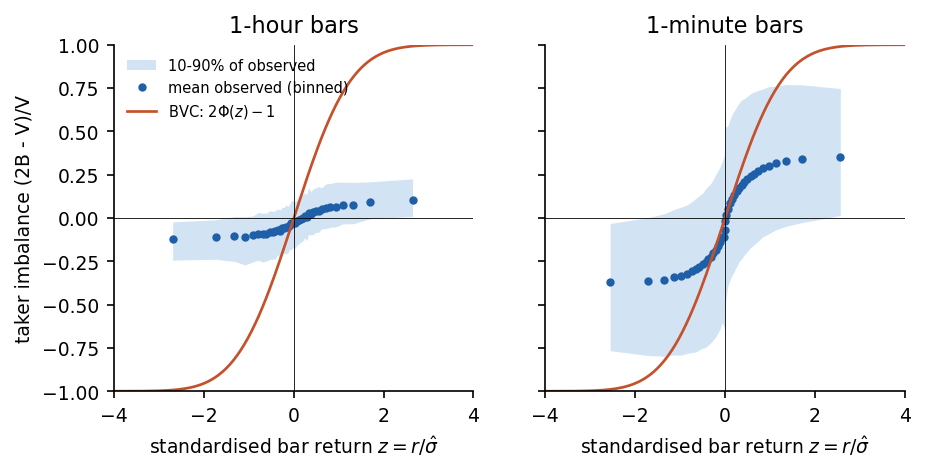
\includegraphics[width=0.85\textwidth]{fig_bvc_calibration.png}
\caption{Observed taker imbalance against the standardised bar return. Dots are bin means of
observed imbalance in 40 quantile bins of $z$; the band covers the 10th to 90th percentile within
each bin; the line is the BVC mapping $2\Phi(z)-1$. BTC/USDT, January 2022 to October 2026.}
\label{fig:calibration}
\end{figure}

\paragraph{Price impact.} Kyle's lambda estimated from BVC-signed dollar volume has a correlation of
only \BTClambdaCorr{} with the same estimator applied to observed signed volume. Errors in the
regressor are amplified in a ratio of a covariance to a variance, so a proxy that captures about
a quarter of the flow variance yields an impact estimate that is largely noise.

\paragraph{Volatility.} The range-based Garman-Klass estimator from hourly bars has a correlation
of \BTCgkCorr{} with realised variance from one-minute returns (both in logs, 24-hour windows).
Bar-based volatility measures are close substitutes for realised measures at this horizon.

\paragraph{Spreads.} The minimum quoted spread on BTC/USDT is one tick of 0.01~USDT, about
\BTCtick{} basis points at the sample's median price. The 24-hour Corwin-Schultz estimate has a median
of \BTCcsMedian{} basis points, so taken at face value it would imply an average book about four
orders of magnitude wider than one tick, an implausible value for the most liquid crypto pair. Its
logarithm has a correlation of \BTCcsVolCorr{} with log realised volatility. The Abdi-Ranaldo
estimate is truncated at zero in \BTCarZero{} of hours and the Roll estimate in \BTCrollZero. In this
market the spread estimators measure volatility, the extreme case of the bias documented by
\citet{jahanparvar2023}. Liquidity conclusions drawn from them at hourly frequency should be read as
volatility conclusions.

\paragraph{Stability.} The BVC correlation varies between \BTCbvcYearMin{} and \BTCbvcYearMax{}
across calendar years and is essentially the same in low-, medium- and high-volatility regimes at
the hourly level (Appendix Table~\ref{tab:regimes}). It is higher during Binance's zero-fee
promotion on BTC/USDT (8 July 2022 to 22 March 2023), when hourly trade counts rose sharply
(\BTCbvcZeroFee{} against \BTCbvcStdFee{} under standard fees). The reason is visible in the
flow itself. During the promotion the standard deviation of hourly taker imbalance on BTC/USDT fell
to \BTCsdImbZero, from \BTCsdImbStd{} under standard fees: volume rose fivefold but became almost
perfectly two-sided, which is what costless round-trip trading produces. On ETH/USDT, which kept its
fees, the dispersion barely changed (\ETHsdImbZero{} against \ETHsdImbStd). With little genuine
directional flow left, the price change of a bar explains a larger share of what remains. The
relation between prices and aggressor flow therefore depends on the exchange's fee schedule and on
the composition of trading it attracts \citep{cong2023}, and data from fee-free periods should be
treated with care.


\section{A natural experiment: what zero fees did to the bars}\label{sec:fee}

The comparisons so far use a sample in which the composition of trading changes slowly. A change in
trading fees gives a sharper test of what bar-based measures respond to. A fee is a cost per unit of
volume, not per unit of information. Removing it makes a round trip, a purchase and an offsetting
sale of the same quantity, nearly free on a pair whose quoted spread is one tick, so it can add
volume and trades without adding net order flow. Measures that scale by volume, such as the Amihud
ratio and the Kyle's lambda and VPIN built from BVC-signed volume, would then register a change in
liquidity or in the toxicity of flow, while measures built from observed net flow would not.
Binance's zero-fee promotion lets us run this test with untreated coins as controls, with switch
times that are known to the hour, and with the reversal of the treatment as a second test.

\subsection{Institutional setting and design}

\paragraph{The promotion.} On 6 July 2022 Binance announced that from 8 July, until further notice,
it would charge neither maker nor taker fees on thirteen spot pairs of bitcoin against stablecoins
and fiat currencies, including BTC/USDT and BTC/BUSD \citep{coindesk2022}. Within hours of the
start, after a surge of trading at almost unchanged prices, the exchange excluded these pairs from
the volume that determines VIP fee tiers, with the stated aim of removing the incentive to wash
trade \citep{decrypt2022}. Standard fees returned on BTC/USDT and the other pairs on 22 March 2023,
except on BTC/TUSD, which stayed free until 7 September 2023
\citep{coindesk2023,cryptonews2023}; by then BTC/FDUSD, which opened in \pairFdusdStart, was
the only bitcoin pair with neither fee \citep{cryptonews2023}. The USDT pairs of other coins paid
standard fees throughout.

\paragraph{Timing.} The switch times can be read off the data (Figure~\ref{fig:switch}). The number
of trades on BTC/USDT jumps between the 13:00 and 14:00 UTC bars of 8 July 2022 and drops at the
00:00 UTC bar of 22 March 2023, while the average control coin does not move. Measured relative to
the controls, BTC trade counts in the 24 hours after the first switch were \feeJumpOnTradesX{} times
those in the 24 hours before, and \feeJumpOffTradesX{} times after the second switch. Over the same
24-hour comparison at \feeJumpPlaceboN{} placebo hours in 2024--2026 the largest absolute change in
log trade counts is \feeJumpPlaceboMax, against \feeJumpOnTradesA{} and \feeJumpOffTradesA{} at the
two switches.

\begin{figure}[t]
\centering
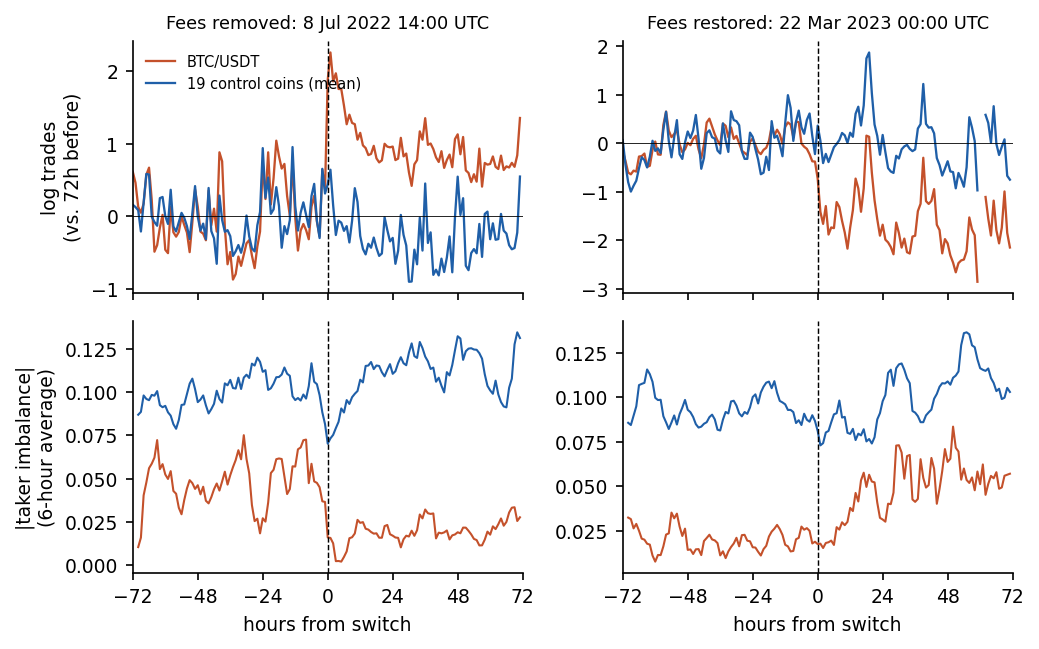
\includegraphics[width=0.95\textwidth]{fig_switch_hours.png}
\caption{Hourly trades and taker imbalance around the two fee switches. Top: log number of trades
relative to the mean over the 72 hours before the switch, for BTC/USDT and for the average of the
\feeNcontrols{} control coins. Bottom: absolute hourly taker imbalance $|2B_t-V_t|/V_t$, six-hour
moving average. The dashed lines mark the first hour without fees (left) and the first hour with
fees again (right).}
\label{fig:switch}
\end{figure}

\paragraph{Daily measures.} For each coin and day we compute, from one-minute bars, the number of
trades, the dollar volume $V$ and the average trade size; the \emph{directional volume}
$\sum_m |B_m-S_m|$ and the \emph{two-sided volume}
\begin{equation}\label{eq:twosided}
V^{\text{2s}}=\sum_m \bigl(B_m+S_m-|B_m-S_m|\bigr)=\sum_m 2\min(B_m,S_m),
\end{equation}
where $B_m$ and $S_m$ are the dollar volumes of buyer- and seller-initiated trades in minute $m$, so
that two-sided volume is the part of the day's volume that is offset by opposite aggressor flow
within the same minute; the mean absolute hourly taker imbalance; realised volatility; the Amihud
ratio from hourly bars; Kyle's lambda as the slope of one-minute returns on signed dollar flow,
with flow signed by BVC and, alternatively, observed; VPIN computed from hourly BVC-signed and from
observed signed volume; the $R^2$ of one-minute returns on observed flow; the correlation of
one-minute BVC imbalance with observed imbalance; and the first-order autocorrelation of one-minute
returns.

\paragraph{Design.} BTC/USDT is the treated unit and the \feeNcontrols{} other USDT pairs of
Section~\ref{sec:data} are the controls. For each measure let $D_d$ be the value for BTC on day $d$
minus the average over the controls (in logarithms for positive quantities), which removes
market-wide movements as day fixed effects would. The effect of a switch is the change in the mean
of $D_d$ from the 90 days before to the 90 days after it, estimated by regressing $D_d$ on an
indicator for the later window with Newey-West standard errors (30 lags); 8 July 2022, which is
split between the two regimes, is left out. With a single treated unit, conventional standard
errors can understate uncertainty \citep{conley2011}, so we add two permutation tests. In the
\emph{in-space} test each control in turn is treated as if it had been treated, with the remaining
controls as its comparison group, and the $p$-value is the rank of BTC's absolute effect among all
\panelN{} coins; the smallest attainable value is \feeMinPspace{} \citep{abadie2010}. In the
\emph{in-time} test the same statistic is computed for BTC at \feeNtime{} weekly placebo dates in
2024--2026, when no fee change affected BTC/USDT, and the $p$-value is the share of placebo effects at
least as large in absolute value. The identifying assumption is that, without the fee change, the
difference between BTC and the average control would not have shifted at the switch. The restoration
of fees provides a second, independent check: a bitcoin-specific shock that happened to coincide with
the removal of fees would have to be undone, at the same hour of the day, eight and a half months
later.

\begin{table}[t]
\centering\caption{Effects of removing and restoring fees on BTC/USDT}\label{tab:feedid}
\resizebox{\textwidth}{!}{\begin{tabular}{lrrrrrrrrr}
\toprule
 & \multicolumn{3}{c}{BTC/USDT, daily median} & \multicolumn{3}{c}{Fees removed} & \multicolumn{3}{c}{Fees restored}\\
\cmidrule(lr){2-4}\cmidrule(lr){5-7}\cmidrule(lr){8-10}Measure & Before & Zero fee & After & $\Delta$ ($t$) & $p_{\text{space}}$ & $p_{\text{time}}$ & $\Delta$ ($t$) & $p_{\text{space}}$ & $p_{\text{time}}$\\
\midrule
\multicolumn{10}{l}{\emph{Panel A. Trading activity}}\\
Trades per day (millions) & 1.12 & 5.74 & 0.82 & 1.68 (12.2) & 0.050 & 0.008 & \ensuremath{-}1.68 (\ensuremath{-}18.1) & 0.050 & 0.008\\
Dollar volume per day (\$bn) & 1.78 & 4.73 & 1.05 & 1.21 (5.9) & 0.100 & 0.008 & \ensuremath{-}1.18 (\ensuremath{-}11.2) & 0.050 & 0.008\\
Average trade size (\$) & 1,566 & 826 & 1,259 & \ensuremath{-}0.46 (\ensuremath{-}4.3) & 0.100 & 0.081 & 0.50 (7.5) & 0.050 & 0.073\\
\multicolumn{10}{l}{\emph{Panel B. Direction of the volume (one-minute taker flow)}}\\
Directional volume $\sum_m|B_m-S_m|$ (\$bn) & 0.44 & 0.55 & 0.36 & 0.43 (3.3) & 0.200 & 0.185 & \ensuremath{-}0.27 (\ensuremath{-}3.1) & 0.350 & 0.565\\
Two-sided volume (\$bn) & 1.35 & 4.20 & 0.70 & 1.43 (6.0) & 0.100 & 0.008 & \ensuremath{-}1.33 (\ensuremath{-}12.0) & 0.050 & 0.008\\
Two-sided share of volume & 0.74 & 0.88 & 0.66 & 0.16 (6.2) & 0.050 & 0.008 & \ensuremath{-}0.15 (\ensuremath{-}8.9) & 0.050 & 0.008\\
Mean $|$hourly taker imbalance$|$ & 0.065 & 0.023 & 0.086 & \ensuremath{-}1.03 (\ensuremath{-}9.3) & 0.050 & 0.008 & 1.15 (21.3) & 0.050 & 0.008\\
\multicolumn{10}{l}{\emph{Panel C. Liquidity and flow measures computed from bars}}\\
Amihud ratio, hourly bars ($|r|$ per \$bn) & 0.064 & 0.013 & 0.052 & \ensuremath{-}1.18 (\ensuremath{-}6.9) & 0.100 & 0.008 & 1.52 (21.8) & 0.050 & 0.008\\
Kyle's $\lambda$, BVC-signed flow (bps per \$M) & 3.81 & 1.53 & 3.05 & \ensuremath{-}0.39 (\ensuremath{-}3.1) & 0.150 & 0.032 & 0.97 (15.2) & 0.050 & 0.008\\
VPIN, BVC & 0.50 & 0.45 & 0.47 & \ensuremath{-}0.10 (\ensuremath{-}4.7) & 0.050 & 0.008 & 0.11 (5.1) & 0.050 & 0.008\\
\multicolumn{10}{l}{\emph{Panel D. The same quantities from observed taker flow}}\\
Kyle's $\lambda$, observed flow (bps per \$M) & 6.29 & 5.55 & 5.90 & 0.24 (1.4) & 0.400 & 0.435 & 0.30 (4.1) & 0.250 & 0.290\\
VPIN, observed flow & 0.069 & 0.023 & 0.083 & \ensuremath{-}1.08 (\ensuremath{-}8.8) & 0.050 & 0.008 & 1.11 (23.1) & 0.050 & 0.008\\
$R^2$ of 1m returns on observed flow & 0.24 & 0.41 & 0.40 & 0.13 (5.2) & 0.050 & 0.008 & \ensuremath{-}0.06 (\ensuremath{-}3.8) & 0.050 & 0.081\\
corr(BVC, observed imbalance), 1m & 0.50 & 0.59 & 0.61 & 0.05 (4.1) & 0.150 & 0.008 & \ensuremath{-}0.05 (\ensuremath{-}6.2) & 0.100 & 0.008\\
\multicolumn{10}{l}{\emph{Panel E. Prices}}\\
Realised volatility (\% per day) & 3.05 & 2.42 & 1.76 & 0.15 (1.4) & 0.900 & 0.742 & 0.48 (1.9) & 0.150 & 0.169\\
First-order autocorrelation of 1m returns & 0.012 & \ensuremath{-}0.002 & 0.016 & \ensuremath{-}0.01 (\ensuremath{-}0.5) & 0.850 & 0.677 & 0.02 (2.0) & 0.250 & 0.306\\
\bottomrule
\end{tabular}
}
\tabnote{Daily medians for BTC/USDT from 1 January to 7 July 2022 (before), 9 July 2022 to 21 March
2023 (zero fee) and 22 March to 6 September 2023 (after). $\Delta$: change in the mean of the
BTC-minus-control difference between the 90 days before and the 90 days after the switch, in log
points for the measures shown in logs (all except the two-sided share, the $R^2$, the correlation
and the autocorrelation, which are in levels), with the Newey-West $t$-statistic in parentheses.
$p_{\text{space}}$: rank of BTC's absolute effect among the \panelN{} coins when each control is
treated in turn as if it had been treated. $p_{\text{time}}$: share of \feeNtime{} placebo dates in
2024--2026 with an absolute effect at least as large.}
\end{table}

\subsection{Results}

\paragraph{Activity.} Table~\ref{tab:feedid} reports the effects. Removing fees multiplied the number
of trades on BTC/USDT by \feeOnTradesX{} and its dollar volume by \feeOnDvolX{} relative to the
controls. Both effects are larger than at any placebo date. The effect on trades is the largest among
the twenty coins; for dollar volume one control, ETC, had a larger change, as its trading surged in
July 2022 ahead of Ethereum's switch to proof of stake, which was expected to send miners to the
Ethereum Classic network. Both effects were reversed when fees returned (\feeOffTrades{} and
\feeOffDvol{} log points), and there BTC's changes are the largest of all coins. The average trade
became smaller.

\paragraph{Where the volume came from.} The new volume had little direction. Two-sided volume rose by
a factor of \feeOnTwoX{} and the two-sided share of volume by \feeOnShare. Directional volume rose by a
factor of \feeOnNetX, but this increase is not significant in either permutation test
($p_{\text{space}}=\feeOnNetPs$, $p_{\text{time}}=\feeOnNetPt$), and neither is the decline when fees
returned; some directional flow may have moved to Binance from other exchanges, whose fees did not
change. Relative to the counterfactual implied by the controls, \feeExcessTwoShare{} of the
additional dollar volume during the promotion was offset within the same minute by opposite aggressor
flow. The mean absolute hourly imbalance fell by
\feeOnImbPctA\% and recovered when fees returned. Trade-level data around the switches
(Table~\ref{tab:forensics}) show the same at a finer scale: the share of BTC/USDT volume offset by
opposite aggressor flow within the \emph{same second} was \tfBtcTwoSecA{} on the two days before the
fees were removed and \tfBtcTwoSecB{} on the two days after, and \tfBtcTwoSecC{} on the two days
before they were restored and \tfBtcTwoSecD{} after; on ETH/USDT it was between \tfEthTwoSecMin{} and
\tfEthTwoSecMax{} on all eight days. Immediate round trips of identical size, a trade followed within
one second by an opposite trade of exactly the same quantity, account for at most \tfBtcPingVolMax{}
of BTC volume on any of these days. The fee-free volume was therefore not a simple repetition of
matched orders but fast two-sided trading in varying sizes, which is what both high-frequency
liquidity provision and wash trading designed to avoid detection would produce
\citep{cong2023,aloosh2024}. Aggressor flags cannot tell the two apart.

\begin{table}[t]
\centering\caption{Trade-level composition of volume around the fee switches}\label{tab:forensics}
\resizebox{\textwidth}{!}{\begin{tabular}{llrrrrrr}
\toprule
Days & Pair & Trades (M/day) & Median trade (\$) & Round trips: trades & volume & Two-sided, 1s & Two-sided, 1m\\
\midrule
fees (before removal) & BTC/USDT & 1.17 & 250 & 1.2\% & 0.1\% & 30\% & 82\%\\
fees (before removal) & ETH/USDT & 0.63 & 470 & 0.5\% & 0.0\% & 32\% & 79\%\\
zero fees (after removal) & BTC/USDT & 3.16 & 204 & 1.4\% & 1.3\% & 59\% & 91\%\\
zero fees (after removal) & ETH/USDT & 0.46 & 285 & 3.7\% & 0.4\% & 20\% & 72\%\\
zero fees (before restoration) & BTC/USDT & 10.38 & 181 & 0.6\% & 0.1\% & 53\% & 92\%\\
zero fees (before restoration) & ETH/USDT & 0.80 & 237 & 0.2\% & 0.2\% & 25\% & 77\%\\
fees (after restoration) & BTC/USDT & 1.37 & 157 & 0.3\% & 0.1\% & 25\% & 76\%\\
fees (after restoration) & ETH/USDT & 0.68 & 343 & 0.3\% & 0.2\% & 26\% & 77\%\\
\bottomrule
\end{tabular}
}
\tabnote{Averages over two days: 6--7 July 2022 (fees), 9--10 July 2022 (zero fees), 20--21 March 2023
(zero fees) and 23--24 March 2023 (fees). Trades are Binance aggregated trades (all fills of one taker
order at one price). Round trips: share of trades, and of dollar volume, that are followed or
preceded within one second by a trade of identical quantity with the opposite aggressor side.
Two-sided: $1-\sum_s|B_s-S_s|/\sum_s(B_s+S_s)$ over seconds or minutes $s$.}
\end{table}

\paragraph{What the bars say.} Bar-based measures read the episode as a large improvement in
liquidity. The Amihud ratio fell by \feeOnAmihudPctA\% relative to the controls and Kyle's lambda
estimated from BVC-signed flow by \feeOnLamBvcPctA\%; both returned towards their earlier levels when
fees were restored. VPIN computed with BVC changed by only \feeOnVpinBvcPct\%, so a researcher using
it would conclude that the toxicity of order flow was unaffected.

\paragraph{What the observed flow says.} Observed flow tells a different story. Price impact per
dollar of observed net flow, Kyle's lambda with observed signing, changed by \feeOnLamTruePct\%
($t=\feeOnLamTrueT$, $p_{\text{space}}=\feeOnLamTruePs$, $p_{\text{time}}=\feeOnLamTruePt$) when
fees were removed and by \feeOffLamTruePct\% when they returned ($p_{\text{space}}=\feeOffLamTruePs$,
$p_{\text{time}}=\feeOffLamTruePt$), and realised volatility did not change significantly at either
switch. VPIN computed from observed flow, by contrast, fell by \feeOnVpinTruePctA\% and recovered at
the restoration: the imbalance of aggressor flow per unit of volume collapsed, because the added
volume was balanced. A dollar of net order flow moved prices at least as much as before, so liquidity
for a trader with a directional order did not improve, whatever the volume measures say; order-book
data indicate that it deteriorated, with wider spreads and less depth \citep{galati2024}. The Amihud
ratio scales price changes by gross volume and VPIN-BVC scales classified flow by gross volume;
neither can tell volume that moves prices from volume that is offset within the minute. The changes
in the Amihud ratio are roughly the sum of the changes in observed-flow lambda and in observed VPIN
(\feeOnLamTrue{} and \feeOnVpinTrue{} log points against \feeOnAmihud{} when fees were removed,
\feeOffLamTrue{} and \feeOffVpinTrue{} against \feeOffAmihud{} when they returned): most of the
movement reflects the share of net flow in volume, not the cost of price impact.

\paragraph{Calibration and information.} The episode also changes the calibration of BVC. Within the
promotion the slope of observed imbalance on hourly BVC was \BTCslopeZero, against \BTCslopeStd{}
under standard fees (Appendix Table~\ref{tab:ceiling}), so a classifier calibrated in one regime
misstates the scale of flow in the other by a factor of about four. Its correlation with observed
imbalance changed little (\feeOnCorr{} and \feeOffCorr{} at the two switches). The $R^2$ of one-minute
returns on observed flow rose by \feeOnRsq{} when fees were removed and fell by \feeOffRsqA{} when they
returned: under zero fees, net taker flow tracked contemporaneous price changes more closely, as it
would if fee-free traders, for example arbitrageurs across the thirteen bitcoin pairs, took liquidity
in the direction of price moves. For aggressor flow we therefore find no sign that zero fees made
order flow less informative about prices, the conclusion \citet{bozzetto2026} reach for order-book
imbalance; the two measures capture different flows.

\subsection{The volume follows the fee}

The strongest evidence that the two-sided volume was a response to fees, and not to anything specific
to bitcoin or to USDT, comes from the other bitcoin pairs (Figure~\ref{fig:pairs} and
Table~\ref{tab:pairs}). While all thirteen pairs were free, BTC/TUSD traded a median of
\$\pairTusdVolB{} million a day. Once it was the only free pair it traded \$\pairTusdVolC{} million,
and its mean absolute hourly imbalance fell from \pairTusdImbB{} to \pairTusdImbC, the level BTC/USDT
had shown while it was free (\pairUsdtImbB). When fees returned on BTC/TUSD in September 2023, the
volume and the same low-imbalance signature moved to BTC/FDUSD (\$\pairFdusdVolD{} million a day,
imbalance \pairFdusdImbD), while the imbalance of BTC/USDT stayed at its pre-promotion level
(\pairUsdtImbA{} before, \pairUsdtImbC{} and \pairUsdtImbD{} after). The same pattern, high volume with
almost perfectly balanced aggressor flow, appeared three times on three different pairs, each time
exactly where trading was free.

\begin{figure}[t]
\centering
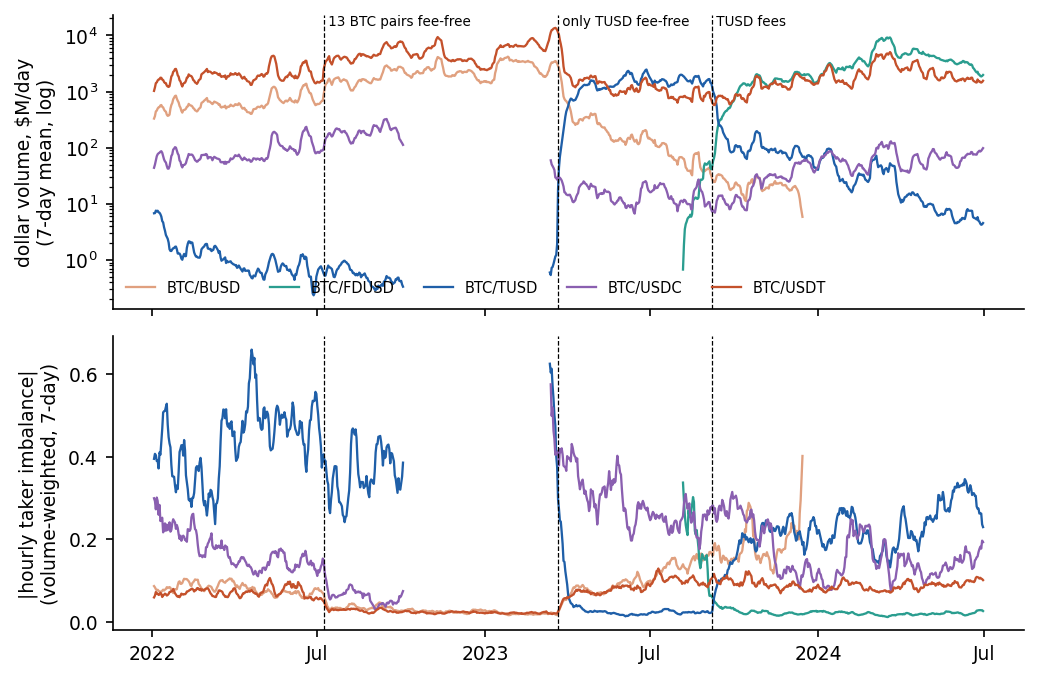
\includegraphics[width=0.95\textwidth]{fig_btc_pairs.png}
\caption{Bitcoin against five stablecoins on Binance: daily dollar volume (top, log scale) and
volume-weighted mean absolute hourly taker imbalance (bottom), seven-day moving averages. Dashed
lines: zero fees on thirteen bitcoin pairs from 8 July 2022; standard fees on all of them except
BTC/TUSD from 22 March 2023; standard fees on BTC/TUSD from 7 September 2023.}
\label{fig:pairs}
\end{figure}

\begin{table}[t]
\centering\caption{Bitcoin pairs by fee regime}\label{tab:pairs}
\resizebox{\textwidth}{!}{\begin{tabular}{lrrrrrrrr}
\toprule
 & \multicolumn{2}{c}{Jan--Jul 2022} & \multicolumn{2}{c}{Jul 2022--Mar 2023} & \multicolumn{2}{c}{Mar--Sep 2023} & \multicolumn{2}{c}{Sep--Dec 2023}\\
 & \multicolumn{2}{c}{\emph{fees on all}} & \multicolumn{2}{c}{\emph{13 pairs free}} & \multicolumn{2}{c}{\emph{only TUSD free}} & \multicolumn{2}{c}{\emph{FDUSD free}}\\
\cmidrule(lr){2-3}\cmidrule(lr){4-5}\cmidrule(lr){6-7}\cmidrule(lr){8-9}Pair & \$M/day & $|$imb.$|$ & \$M/day & $|$imb.$|$ & \$M/day & $|$imb.$|$ & \$M/day & $|$imb.$|$\\
\midrule
BTC/USDT & 1,784 & 0.072 & 4,728 & 0.024 & 1,055 & 0.086 & 1,060 & 0.091\\
BTC/BUSD & 592 & 0.080 & 2,231 & 0.027 & 132 & 0.107 & 20 & 0.196\\
BTC/TUSD & 0.9 & 0.437 & 0.5 & 0.368 & 1,419 & 0.030 & 82 & 0.196\\
BTC/FDUSD & -- & -- & -- & -- & 9.9 & 0.181 & 1,371 & 0.025\\
BTC/USDC & 71 & 0.172 & 170 & 0.101 & 13 & 0.287 & 25 & 0.195\\
\bottomrule
\end{tabular}
}
\tabnote{Median daily dollar volume (\$ million) and mean volume-weighted absolute hourly taker
imbalance of each pair, by fee regime. In the second window all five pairs were free; in the third only
BTC/TUSD was; in the fourth BTC/FDUSD was the only pair without fees. BTC/FDUSD opened in
\pairFdusdStart.}
\end{table}

\subsection{Robustness and implications}

Appendix Table~\ref{tab:feerobust} repeats the estimates with ETH/USDT as the only control, with 60-
and 180-day windows, and with a comparison of the full windows before, during and after the
promotion, with and without a linear trend in the BTC-minus-control difference. The effects on
activity, on the composition of volume and on the bar-based measures keep their sign in every
specification and are significant at the 5\% level in all but one case, the fall of BVC-based lambda
in the full-window regression with a trend. The change in observed-flow lambda, by contrast, takes
both signs across specifications. The event-study plots in Appendix Figure~\ref{fig:feeevent} show
that the effects appear and disappear at the switch dates.

Two implications follow. First, volume-based liquidity measures are not comparable across fee
regimes, exchanges or periods with different incentives to trade for its own sake. In
cryptocurrency markets, where fee promotions, volume-based fee tiers and wash trading are common
\citep{cong2023,amiram2025}, a fall in the Amihud ratio or in BVC-based lambda can mean that more
volume is being offset within the minute rather than that liquidity has improved. Second, in the
data that zero fees produce, the aggressor imbalance of a bar is diluted by two-sided trading, and
the bar's volume says little about how much of it carried direction. Exchange-reported aggressor
flow reveals the dilution; bars alone cannot.


\section{What does order flow tell us about future prices?}\label{sec:response}

Before turning to out-of-sample forecasting, we ask a simpler question: is the observed flow, or its
proxy, related to subsequent returns at all, and if so, through which component? For each horizon
$k=1,\dots,24$ hours we estimate
\begin{equation}\label{eq:response}
\log\frac{C_{t+k}}{C_t}\times 10^4 = a_k + b_k\,\tilde x_t + c_k\,\tilde z_t + e_{t,k},
\end{equation}
where $\tilde x_t$ is a standardised flow measure of bar $t$ (observed taker imbalance or BVC
imbalance) and $\tilde z_t$ the standardised bar return $r_t/\hat\sigma_t$, which is the only input of
BVC. The coefficient $b_k$ is the cumulative return, in basis points, that follows a one standard
deviation flow shock. When $\tilde z_t$ is included, $b_k$ measures the effect of the component of
flow that is orthogonal to the bar's own price change, i.e.\ the part that no return-based classifier
can recover. Standard errors are Newey-West with $\max(24,2k)$ lags. These regressions use the full
sample and are descriptive; Section~\ref{sec:forecast} asks whether anything survives out of sample.

\begin{figure}[t]
\centering
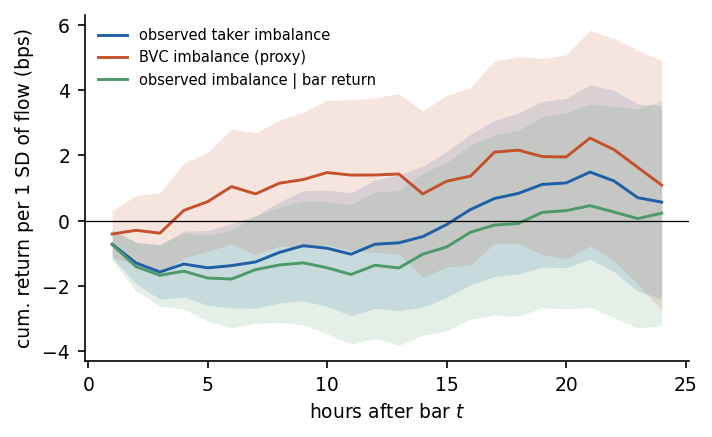
\includegraphics[width=0.7\textwidth]{fig_flow_response.png}
\caption{Cumulative log return (basis points) over $k$ hours following a one standard deviation flow
shock in hour $t$, from regression~\eqref{eq:response}, with 95\% Newey-West bands. Blue: observed
taker imbalance alone. Red: BVC imbalance alone. Green: observed imbalance holding the bar's
standardised return fixed. BTC/USDT.}
\label{fig:response}
\end{figure}

\begin{table}[t]
\centering\caption{Return response to order-flow shocks, BTC/USDT}\label{tab:response}
\begin{tabular}{lrrrrrr}
\toprule
Regressor (1 SD) & $k=1$h & $k=2$h & $k=4$h & $k=8$h & $k=12$h & $k=24$h\\
\midrule
Observed taker imbalance & \ensuremath{-}0.72 & \ensuremath{-}1.30 & \ensuremath{-}1.33 & \ensuremath{-}0.97 & \ensuremath{-}0.72 & 0.57\\
 & (\ensuremath{-}3.42) & (\ensuremath{-}3.99) & (\ensuremath{-}2.58) & (\ensuremath{-}1.23) & (\ensuremath{-}0.72) & (0.38)\\
BVC imbalance & \ensuremath{-}0.41 & \ensuremath{-}0.30 & 0.31 & 1.15 & 1.40 & 1.09\\
 & (\ensuremath{-}1.12) & (\ensuremath{-}0.55) & (0.42) & (1.17) & (1.16) & (0.56)\\
Observed imbalance, given $z_t$ & \ensuremath{-}0.73 & \ensuremath{-}1.41 & \ensuremath{-}1.55 & \ensuremath{-}1.36 & \ensuremath{-}1.37 & 0.23\\
 & (\ensuremath{-}2.97) & (\ensuremath{-}3.74) & (\ensuremath{-}2.61) & (\ensuremath{-}1.51) & (\ensuremath{-}1.20) & (0.13)\\
Bar return $z_t$, given imbalance & 0.02 & 0.26 & 0.50 & 0.89 & 1.48 & 0.78\\
 & (0.06) & (0.46) & (0.64) & (0.84) & (1.15) & (0.38)\\
\bottomrule
\end{tabular}

\tabnote{Coefficients from regression~\eqref{eq:response}: cumulative log return in basis points from
the close of hour $t$ to $t+k$ per one standard deviation of the regressor; Newey-West $t$-statistics
in parentheses. The third and fourth rows come from one regression with both regressors.}
\end{table}

Figure~\ref{fig:response} and Table~\ref{tab:response} show three facts. First, observed aggressor
flow predicts a \emph{reversal}. A one standard deviation increase in taker imbalance is followed by
a price decline of \BTCfrTakAone{} basis points over the next hour ($t=\BTCfrTakTone$) and \BTCfrTakAtwo{}
basis points over two hours ($t=\BTCfrTakTtwo$); the decline is \BTCfrTakAfour{} basis points at four
hours and has disappeared after about 15 hours. Buying pressure that is absorbed by passive orders is
followed by falling prices, which is consistent with a transient component of price impact
\citep{bouchaud2018} and with passive liquidity providers being, on average, on the right side of
the trade.

Second, the information is in the part of flow that the bar's price does not reveal. Holding the
standardised bar return fixed leaves the coefficient on observed imbalance essentially unchanged
(\BTCfrJointBtwo{} basis points at two hours, $t=\BTCfrJointTtwo$), while the bar return itself has no
predictive power ($t=\BTCfrZTtwo$ at two hours and $t=\BTCfrZTfour$ at four). Third, and as a
consequence, hourly BVC imbalance predicts nothing: its coefficient is \BTCfrBvcBtwo{} basis points at
two hours ($t=\BTCfrBvcTtwo$) and is positive, if insignificant, at longer horizons.
Section~\ref{sec:validation} showed that about three-quarters of the variance of observed imbalance
is invisible in the hourly bar's price change; this section shows that the invisible part is the part
that matters.

\paragraph{Controls and the best available proxy.} Table~\ref{tab:controls} asks whether the reversal
is a disguised return or volume effect. Adding three lags of the hourly return, 24-hour momentum,
standardised volume, volatility and the previous hour's imbalance leaves the two-hour coefficient at
\BTCrcctrlB{} basis points ($t=\BTCrcctrlT$). The flow effect is not a reversal of past returns and
not a volume or volatility effect. The last rows use the most accurate proxy we can build from price
data, BVC applied to one-minute bars and summed to the hour, whose correlation with observed
imbalance is \BTCbvcOneMinCorr{} rather than \BTCbvcCorr. On its own it does predict a reversal
(\BTCrcbvcmB{} basis points at two hours, $t=\BTCrcbvcmT$). When it competes with observed imbalance,
however, its coefficient falls to \BTCrcvsBvcmB{} ($t=\BTCrcvsBvcmT$) while observed imbalance keeps
\BTCrcvsTakB{} ($t=\BTCrcvsTakT$). Predictive content therefore rises with measurement accuracy: none
for hourly BVC, part of the signal for one-minute BVC, and all of it for observed flow, which subsumes
the proxy.

\begin{table}[t]
\centering\caption{Return response to observed flow with controls and against the best proxy}\label{tab:controls}
\resizebox{\textwidth}{!}{\begin{tabular}{lrrr}
\toprule
Specification (coefficient of interest) & $k=1$h & $k=2$h & $k=4$h\\
\midrule
\multicolumn{4}{l}{\emph{BTC/USDT}}\\
(1) taker & \ensuremath{-}0.72 (\ensuremath{-}3.4) & \ensuremath{-}1.30 (\ensuremath{-}4.0) & \ensuremath{-}1.33 (\ensuremath{-}2.6)\\
(2) + bar return & \ensuremath{-}0.73 (\ensuremath{-}3.0) & \ensuremath{-}1.41 (\ensuremath{-}3.7) & \ensuremath{-}1.55 (\ensuremath{-}2.6)\\
(3) + lagged returns, 24h momentum & \ensuremath{-}0.73 (\ensuremath{-}2.9) & \ensuremath{-}1.39 (\ensuremath{-}3.6) & \ensuremath{-}1.52 (\ensuremath{-}2.5)\\
(4) + volume, volatility, lagged taker & \ensuremath{-}0.64 (\ensuremath{-}2.5) & \ensuremath{-}1.32 (\ensuremath{-}3.7) & \ensuremath{-}1.52 (\ensuremath{-}2.8)\\
(5) 1m BVC alone & \ensuremath{-}0.65 (\ensuremath{-}2.4) & \ensuremath{-}1.00 (\ensuremath{-}2.5) & \ensuremath{-}0.75 (\ensuremath{-}1.3)\\
(6) taker vs 1m BVC: taker & \ensuremath{-}0.52 (\ensuremath{-}1.9) & \ensuremath{-}1.09 (\ensuremath{-}2.6) & \ensuremath{-}1.38 (\ensuremath{-}2.1)\\
(6) taker vs 1m BVC: 1m BVC & \ensuremath{-}0.33 (\ensuremath{-}1.0) & \ensuremath{-}0.35 (\ensuremath{-}0.7) & 0.09 (0.1)\\
\multicolumn{4}{l}{\emph{ETH/USDT}}\\
(1) taker & 0.10 (0.3) & \ensuremath{-}0.53 (\ensuremath{-}1.1) & 0.55 (0.8)\\
(2) + bar return & \ensuremath{-}0.15 (\ensuremath{-}0.4) & \ensuremath{-}0.79 (\ensuremath{-}1.5) & 0.21 (0.3)\\
(3) + lagged returns, 24h momentum & \ensuremath{-}0.13 (\ensuremath{-}0.4) & \ensuremath{-}0.75 (\ensuremath{-}1.4) & 0.24 (0.3)\\
(4) + volume, volatility, lagged taker & 0.00 (0.0) & \ensuremath{-}0.82 (\ensuremath{-}1.7) & 0.08 (0.1)\\
(5) 1m BVC alone & 0.33 (0.9) & \ensuremath{-}0.23 (\ensuremath{-}0.4) & 0.24 (0.3)\\
(6) taker vs 1m BVC: taker & \ensuremath{-}0.12 (\ensuremath{-}0.4) & \ensuremath{-}0.59 (\ensuremath{-}1.1) & 0.60 (0.7)\\
(6) taker vs 1m BVC: 1m BVC & 0.40 (0.9) & 0.10 (0.2) & \ensuremath{-}0.09 (\ensuremath{-}0.1)\\
\bottomrule
\end{tabular}
}
\tabnote{Coefficient (basis points per standard deviation) of observed taker imbalance, or of
one-minute BVC imbalance where indicated, in regressions of the $k$-hour return on standardised
regressors; Newey-West $t$-statistics in parentheses. (2) adds the standardised bar return; (3)
adds three lagged hourly returns and 24-hour momentum; (4) adds standardised volume, Garman-Klass
volatility and the previous hour's imbalance; (5) uses one-minute BVC imbalance alone; (6) includes
observed and one-minute BVC imbalance together.}
\end{table}

The magnitude is small. At four hours the observed-imbalance regression explains
\BTCfrRtwoFour\% of the return variance, and the implied move of one to two basis points per standard
deviation compares with a standard spot fee of ten basis points per side. Even a perfect measurement
of flow at this frequency would therefore be of little direct use for trading, a conclusion the next
section confirms out of sample.


\section{Out-of-sample forecasting and economic value}\label{sec:forecast}

\subsection{Design}

\paragraph{Target and walk-forward.} The target is the four-hour log return
$y_{t}=\log C_{t+4}-\log C_t$, formed at the close of hour $t$. The first six months after the
feature warm-up are used only for training. The remaining sample (\BTCoosStart{} to \BTCoosEnd,
\BTCnOOS{} hours) is cut into \BTCnFoldsWF{} consecutive 30-day test blocks. Before each block every
model is re-estimated on all observations whose label is observable at the block start, i.e.\ with
$t+4$ strictly before the block (purging); nothing from the block enters estimation. Within each
training window the last 20\% serves as a validation block, itself purged from the inner training
rows, on which hyper-parameters are chosen before the model is refitted on the full window.
Winsorisation bounds (1st and 99th percentiles) and standardisation moments are estimated on the
training window only. Automated tests replace every bar after $t$ by noise and verify that features
at $t$ are unchanged, and check the purge condition for every fold (Appendix~\ref{app:leakage}).

\paragraph{Models.} Following \citet{gu2020}, models forecast the return relative to zero. The
elastic net is fitted without intercept on standardised features, with the penalty chosen from a
13-point grid and the $\ell_1$ share from $\{0.1,0.5,0.9\}$ on the validation block. As a non-linear
benchmark we use gradient-boosted trees with depth three, at least 300 observations per leaf and a
learning rate of 0.03, with the number of rounds chosen on the validation block. We also report the
historical-mean forecast. We estimate every model on every feature set defined in
Section~\ref{sec:measures} and report all of them.

\paragraph{Statistical evaluation.} The out-of-sample $R^2$ relative to a benchmark $b$ is
$R^2_{OOS}=1-\sum(y-\hat y)^2/\sum(y-\hat y^{b})^2$ \citep{campbell2008}. Because the zero forecast and
smaller feature sets are nested in larger ones, we test equal predictive accuracy with the
\citet{clark2007} statistic (one-sided), which adjusts for the noise that estimating irrelevant
parameters adds to the larger model, and report the \citet{diebold1995} statistic, which compares
realised accuracy. Overlapping four-hour targets make forecast errors serially correlated, so all
$t$-statistics use \citet{newey1987} standard errors with $\max(24,2h)$ lags. The information
coefficient (rank correlation of forecast and outcome) is reported with a 95\% moving-block bootstrap
interval with 48-hour blocks \citep{kunsch1989}.

\paragraph{Economic evaluation.} Each hour a signal $s_t\in\{-1,0,1\}$ is formed and held for four
hours with a quarter of capital per sleeve \citep{jegadeesh1993}, so the position over $(t,t+1]$ is
$\frac14\sum_{k=0}^{3}s_{t-k}$; every forecast is used and no exposure is double counted. The
\emph{sign} rule sets $s_t=\operatorname{sign}(\hat y_t)$, which is zero when the model predicts
exactly zero; the \emph{selective} rule trades only when $|\hat y_t|$ exceeds the 80th percentile of
the model's absolute in-sample forecasts in the current training window. Costs of
$c\in\{0,2,5,10\}$ basis points are charged per unit change in position. We report the break-even cost
at which net profit is zero, the HAC $t$-statistic of the intercept in a regression of strategy
returns on BTC returns, the number of calendar years with a positive Sharpe ratio, and the deflated
Sharpe ratio (DSR) of \citet{bailey2014}. The DSR is the probability that a strategy's true Sharpe ratio
exceeds the maximum expected among all \BTCnTrials{} model and rule combinations under the null of no
skill, given their dispersion, the sample length and the non-normality of returns.

\subsection{Forecast accuracy}

\begin{table}[t]
\centering\caption{Out-of-sample forecast accuracy, four-hour BTC/USDT returns}\label{tab:forecast}
\resizebox{\textwidth}{!}{\begin{tabular}{lrrrrcrr}
\toprule
Model & $R^2_{OOS}$ vs.\ 0 (\%) & $R^2_{OOS}$ vs.\ mean (\%) & CW $t$ vs.\ 0 & IC & 95\% CI & Hit rate & Hit $t$\\
\midrule
Historical mean & \ensuremath{-}0.075 & 0.000 & -- & \ensuremath{-}0.002 & [\ensuremath{-}0.021, 0.015] & -- & --\\
EN: TI & \ensuremath{-}0.055 & 0.020 & 1.40$^{*}$ & 0.002 & [\ensuremath{-}0.014, 0.019] & 0.491 & \ensuremath{-}2.14\\
EN: MS$_{\text{proxy}}$ & \ensuremath{-}0.139 & \ensuremath{-}0.064 & \ensuremath{-}0.61$$ & \ensuremath{-}0.005 & [\ensuremath{-}0.024, 0.013] & 0.488 & \ensuremath{-}2.05\\
EN: MS & \ensuremath{-}0.006 & 0.070 & 0.86$$ & \ensuremath{-}0.002 & [\ensuremath{-}0.019, 0.014] & 0.494 & \ensuremath{-}0.92\\
EN: ALL & \ensuremath{-}0.025 & 0.050 & 1.34$^{*}$ & 0.019 & [0.004, 0.035] & 0.508 & 1.44\\
EN: Flow$_{\text{BVC}}$ & \ensuremath{-}0.081 & \ensuremath{-}0.005 & \ensuremath{-}1.35$$ & \ensuremath{-}0.021 & [\ensuremath{-}0.038, \ensuremath{-}0.006] & 0.475 & \ensuremath{-}3.99\\
EN: Flow$_{\text{taker}}$ & \ensuremath{-}0.036 & 0.040 & \ensuremath{-}0.41$$ & \ensuremath{-}0.007 & [\ensuremath{-}0.021, 0.009] & 0.492 & \ensuremath{-}1.26\\
GBM: MS & \ensuremath{-}0.284 & \ensuremath{-}0.208 & 0.39$$ & 0.000 & [\ensuremath{-}0.018, 0.019] & 0.498 & \ensuremath{-}0.66\\
GBM: ALL & \ensuremath{-}0.262 & \ensuremath{-}0.187 & 0.98$$ & 0.003 & [\ensuremath{-}0.014, 0.020] & 0.494 & \ensuremath{-}1.72\\
\bottomrule
\end{tabular}
}
\tabnote{Monthly expanding-window walk-forward, \BTCoosStart{} to \BTCoosEnd{} (\BTCnOOS{} hourly
forecasts). EN: elastic net; GBM: gradient-boosted trees. CW: Clark-West statistic against the zero
forecast (one-sided). IC: Spearman correlation of forecast and outcome, with 95\% block-bootstrap
interval. Hit $t$: HAC $t$-statistic of the hit rate against 50\%. $^{*}$, $^{**}$, $^{***}$: 10\%,
5\%, 1\% significance.}
\end{table}

Table~\ref{tab:forecast} reports the main results for BTC/USDT. All \BTCnModels{} models have a
negative out-of-sample $R^2$ against the zero forecast; the best is \BTCbestRtwoModel{} at
\BTCbestRtwo\%. The historical mean is also worse than zero: trailing average returns are a noisy
estimate of the drift, and in this sample the early training windows are dominated by the 2022 bear
market, which the following recovery reversed \citep{campbell2008}. Clark-West statistics against zero
are significant at the 10\% level only for the technical-indicator model (\(p=\BTCcwpTI\)) and the
full model (\(p=\BTCcwpALL\)). The information coefficients are all within about two hundredths of
zero. The confidence interval excludes zero for the full model ($\text{IC}=\BTCicALL$) and, with the
wrong sign, for the BVC-flow model ($\text{IC}=\BTCicFLOWproxy$), whose coefficients are unstable
across folds. The
observed-flow model, which uses the matched constructions from exchange-reported taker volume, does
no better than its BVC counterpart.

Figure~\ref{fig:cumsse} plots the cumulative difference in squared errors between the zero forecast
and each model \citep{goyal2008}. No line trends upwards for an extended period; gains in some
months are offset by losses in others.

\begin{figure}[t]
\centering
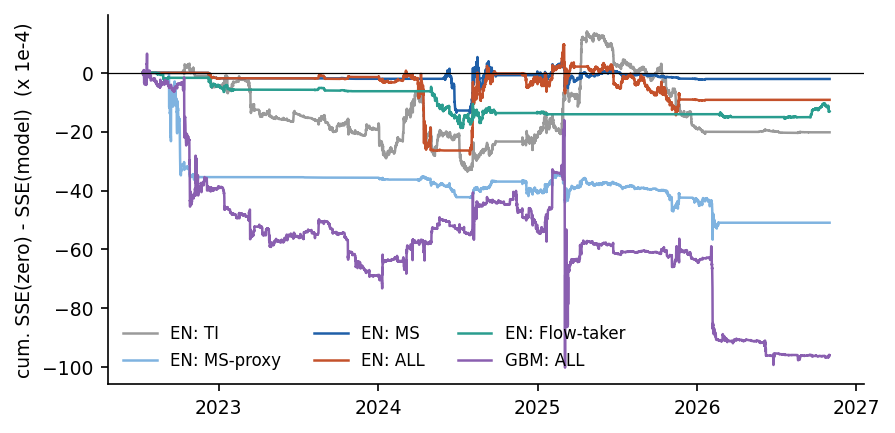
\includegraphics[width=0.8\textwidth]{fig_cum_sse.png}
\caption{Cumulative squared-error difference between the zero forecast and each model, BTC/USDT
four-hour returns. A rising line means the model is more accurate than the zero forecast.}
\label{fig:cumsse}
\end{figure}

\subsection{Incremental information}

\begin{table}[t]
\centering\caption{Incremental predictive information, BTC/USDT}\label{tab:incremental}
\resizebox{\textwidth}{!}{\begin{tabular}{llcrrrrr}
\toprule
Model & Benchmark & Nested & $R^2_{OOS}$ rel.\ (\%) & CW $t$ & CW $p$ & DM $t$ & DM $p$\\
\midrule
EN: ALL & EN: TI & yes & 0.030 & 2.41$^{***}$ & 0.008 & 0.33$$ & 0.741\\
EN: MS & EN: TI & yes & 0.050 & 2.85$^{***}$ & 0.002 & 0.55$$ & 0.585\\
EN: MS & EN: MS$_{\text{proxy}}$ & yes & 0.133 & 2.59$^{***}$ & 0.005 & 1.53$$ & 0.125\\
EN: MS$_{\text{proxy}}$ & EN: TI & yes & \ensuremath{-}0.084 & 1.49$^{*}$ & 0.068 & \ensuremath{-}0.71$$ & 0.476\\
GBM: ALL & EN: TI & yes & \ensuremath{-}0.207 & 1.73$^{**}$ & 0.042 & \ensuremath{-}0.88$$ & 0.378\\
EN: Flow$_{\text{taker}}$ & EN: Flow$_{\text{BVC}}$ & no & 0.045 & -- & -- & 0.97$$ & 0.332\\
\bottomrule
\end{tabular}
}
\tabnote{$R^2_{OOS}$ rel.: out-of-sample $R^2$ of the model relative to the benchmark. CW: Clark-West
test of the null that the larger model adds nothing to the nested benchmark (one-sided). DM:
Diebold-Mariano test of equal mean squared error (two-sided). The observed-flow and BVC-flow models are
not nested, so only DM is reported.}
\end{table}

Table~\ref{tab:incremental} asks whether each richer feature set improves on a simpler one. The
Clark-West test rejects the null that microstructure variables add nothing to technical indicators
($p=\BTCincMSTICWp$ for MS over TI and $p=\BTCincALLTICWp$ for ALL over TI) and that observed flow and
intrahour measures add nothing to the OHLCV proxies ($p=\BTCincMSMSproxyCWp$). In each case, however,
the realised gain in mean squared error is a few hundredths of a percent and the Diebold-Mariano test
does not reject equal accuracy. This is the pattern Clark-West is designed to detect: the larger
model's population coefficients are not all zero, but the information they carry is smaller than the
noise introduced by estimating them, so the larger model does not forecast better in practice.

The model selection inside each training window tells the same story. For the elastic net the
validation step chooses the penalty that sets every coefficient to zero in \BTCnullMSproxy{} of the
\BTCnFolds{} folds with the OHLCV proxies, \BTCnullMS{} with observed flow and intrahour measures, and
\BTCnullALL{} with all features, against \BTCnullTI{} with technical indicators alone. Most of the
time, the data prefer no forecast at all.

\subsection{A single predictor: observed flow against its proxy}

The flow models above combine five constructions and tune a penalty on a short validation block,
which may discard a weak but genuine signal. Section~\ref{sec:response} suggests a direct test: does
the current hour's observed taker imbalance, on its own, forecast returns out of sample, and does its
BVC counterpart? For each predictor we estimate a one-variable regression without intercept on the
standardised predictor in the same expanding monthly walk-forward, with purged labels and moments
from the training window only, and no tuning.

\begin{table}[t]
\centering\caption{Single-predictor out-of-sample test}\label{tab:single}
\resizebox{\textwidth}{!}{\begin{tabular}{lrrrrrrr}
\toprule
 & & & & & & \multicolumn{2}{c}{$R^2_{OOS}$ (CW $p$) by half}\\
\cmidrule(lr){7-8}Predictor & Horizon & $R^2_{OOS}$ (\%) & CW $t$ & CW $p$ & IC & first & second\\
\midrule
\multicolumn{8}{l}{\emph{BTC/USDT}}\\
Observed taker imbalance & 1h & 0.012 & 3.19$^{***}$ & 0.0007 & 0.048 & 0.009 (0.032) & 0.016 (0.005)\\
Observed taker imbalance & 2h & 0.021 & 3.80$^{***}$ & 0.0001 & 0.044 & 0.007 (0.022) & 0.038 (0.001)\\
Observed taker imbalance & 4h & 0.016 & 2.62$^{***}$ & 0.0044 & 0.033 & 0.003 (0.233) & 0.032 (0.006)\\
BVC imbalance (1h bars) & 1h & \ensuremath{-}0.001 & 0.74$$ & 0.2286 & 0.030 & 0.007 (0.183) & \ensuremath{-}0.011 (0.370)\\
BVC imbalance (1h bars) & 2h & \ensuremath{-}0.007 & \ensuremath{-}0.56$$ & 0.7119 & 0.015 & \ensuremath{-}0.010 (0.848) & \ensuremath{-}0.004 (0.489)\\
BVC imbalance (1h bars) & 4h & \ensuremath{-}0.008 & \ensuremath{-}0.35$$ & 0.6353 & \ensuremath{-}0.034 & \ensuremath{-}0.007 (0.484) & \ensuremath{-}0.010 (0.836)\\
BVC imbalance (1m bars) & 1h & 0.014 & 2.39$^{***}$ & 0.0085 & 0.060 & 0.027 (0.015) & 0.000 (0.111)\\
BVC imbalance (1m bars) & 2h & 0.017 & 2.55$^{***}$ & 0.0053 & 0.054 & 0.023 (0.020) & 0.009 (0.062)\\
BVC imbalance (1m bars) & 4h & 0.002 & 1.04$$ & 0.1498 & 0.038 & \ensuremath{-}0.001 (0.319) & 0.005 (0.170)\\
\multicolumn{8}{l}{\emph{ETH/USDT}}\\
Observed taker imbalance & 1h & \ensuremath{-}0.013 & 0.63$$ & 0.2652 & \ensuremath{-}0.035 & \ensuremath{-}0.025 (0.227) & \ensuremath{-}0.003 (0.911)\\
Observed taker imbalance & 2h & \ensuremath{-}0.006 & 0.14$$ & 0.4443 & 0.002 & \ensuremath{-}0.018 (0.616) & 0.004 (0.198)\\
Observed taker imbalance & 4h & \ensuremath{-}0.015 & \ensuremath{-}0.69$$ & 0.7560 & \ensuremath{-}0.016 & \ensuremath{-}0.031 (0.772) & \ensuremath{-}0.002 (0.499)\\
BVC imbalance (1h bars) & 1h & \ensuremath{-}0.006 & 0.42$$ & 0.3383 & \ensuremath{-}0.040 & \ensuremath{-}0.023 (0.448) & 0.008 (0.127)\\
BVC imbalance (1h bars) & 2h & \ensuremath{-}0.004 & 0.41$$ & 0.3405 & \ensuremath{-}0.043 & \ensuremath{-}0.005 (0.358) & \ensuremath{-}0.004 (0.423)\\
BVC imbalance (1h bars) & 4h & 0.009 & 1.20$$ & 0.1151 & \ensuremath{-}0.026 & \ensuremath{-}0.011 (0.620) & 0.025 (0.063)\\
BVC imbalance (1m bars) & 1h & \ensuremath{-}0.005 & \ensuremath{-}0.12$$ & 0.5462 & \ensuremath{-}0.018 & \ensuremath{-}0.011 (0.612) & 0.001 (0.373)\\
BVC imbalance (1m bars) & 2h & \ensuremath{-}0.005 & \ensuremath{-}0.54$$ & 0.7052 & 0.023 & \ensuremath{-}0.007 (0.733) & \ensuremath{-}0.003 (0.562)\\
BVC imbalance (1m bars) & 4h & \ensuremath{-}0.006 & \ensuremath{-}1.19$$ & 0.8829 & 0.013 & \ensuremath{-}0.010 (0.850) & \ensuremath{-}0.004 (0.725)\\
\bottomrule
\end{tabular}
}
\tabnote{One-variable expanding-window regression, re-estimated monthly with purged labels; the
coefficient is learned from past data only. $R^2_{OOS}$ against the zero forecast; CW: Clark-West
test against zero (one-sided); IC: Spearman correlation of forecast and outcome. The last two columns
split the out-of-sample period into halves.}
\end{table}

Table~\ref{tab:single} gives a clean contrast for BTC. Observed taker imbalance has a positive
out-of-sample $R^2$ at every horizon, \BTCspRtwo\% at two hours with a Clark-West $p$-value of
\BTCspPtwo{} and an information coefficient of \BTCspICtwo. The result holds in both halves of the
test period (\BTCspRAtwo\% with $p=\BTCspPAtwo$ in the first and \BTCspRBtwo\% with $p=\BTCspPBtwo$ in
the second). Hourly BVC imbalance has a negative out-of-sample $R^2$ at every horizon and no
significant Clark-West statistic. BVC on one-minute bars lies in between, with an out-of-sample $R^2$
of \BTCspbvcmRtwo\% at two hours ($p=\BTCspbvcmPtwo$), in line with the in-sample gradient of
Section~\ref{sec:response}. Because the coefficient is re-estimated from past data each month, the
sign of the relation is learned in real time; the predictor itself, however, was suggested by the
full-sample analysis, so the test is not pre-registered. Even a Bonferroni correction for all \nALL{}
candidate features leaves the two-hour result for observed flow significant at the 1\% level. For
ETH none of the three predictors forecasts returns, consistent with the weaker in-sample response.

\begin{table}[t]
\centering\caption{Trading on the single observed-flow forecast, two-hour holding period}\label{tab:single_trading}
\begin{tabular}{llrrrrrr}
\toprule
 & & Ann.\ ret.\ (\%) & \multicolumn{3}{c}{Sharpe at cost (bps)} & Turnover & Break-even\\
\cmidrule(lr){4-6} Asset & Rule & gross & 0 & 1 & 2 & per day & (bps)\\
\midrule
BTC/USDT & sign & 30.0 & 0.87 & \ensuremath{-}0.34 & \ensuremath{-}1.54 & 11.4 & 0.72\\
BTC/USDT & selective & 26.4 & 1.43 & 0.23 & \ensuremath{-}0.97 & 6.1 & 1.19\\
ETH/USDT & sign & 10.6 & 0.23 & \ensuremath{-}0.67 & \ensuremath{-}1.56 & 11.3 & 0.26\\
ETH/USDT & selective & 5.9 & 0.26 & \ensuremath{-}0.62 & \ensuremath{-}1.50 & 5.4 & 0.30\\
\bottomrule
\end{tabular}

\tabnote{Overlapping-sleeve rule on the out-of-sample forecast from observed taker imbalance alone
(Table~\ref{tab:single}, two-hour horizon). Sign: trade every hour in the direction of the forecast;
selective: only when $|\hat y_t|$ exceeds the 80th percentile of in-sample absolute forecasts.
Break-even: cost per unit turnover at which net profit is zero.}
\end{table}

Two lessons follow. First, the information that order flow carries about short-horizon BTC returns
is detectable out of sample when flow is measured, partly recoverable from one-minute prices, and
absent from hourly bars. Second, the multivariate elastic net that includes the same variable fails
to exploit it: with a weak signal and many correlated candidates, cross-validated shrinkage on a short
validation block usually selects the empty model. The signal is nonetheless far too small to trade.
Table~\ref{tab:single_trading} applies the overlapping-sleeve rule to the observed-flow forecast with a
two-hour holding period. Gross Sharpe ratios are \BTCstSRsign{} for the sign rule and
\BTCstSRselective{} for the selective rule, but the rules turn over their position many times a day,
and their break-even costs are \BTCstBEsign{} and \BTCstBEselective{} basis points per unit of
turnover. That is an order of magnitude below the standard fee of ten basis points, and below the
taker fees of high-volume accounts, which remain at a few basis points; a strategy that must trade
immediately on an hourly signal cannot rely on maker rebates. The predictable component is a
statistical regularity, not an exploitable strategy.

\subsection{Economic value}

\begin{table}[t]
\centering\caption{Trading performance of forecast-based rules, BTC/USDT}\label{tab:backtest}
\resizebox{\textwidth}{!}{\begin{tabular}{lrrrrrrrcr}
\toprule
& Ann.\ ret.\ (\%) & \multicolumn{3}{c}{Sharpe at cost (bps)} & Turnover & Break-even & $\alpha$ $t$ & Years & DSR\\
\cmidrule(lr){3-5} Model & gross & 0 & 2 & 5 & per day & (bps) & (HAC) & $SR>0$ & \\
\midrule
\multicolumn{10}{l}{\emph{Sign rule}}\\
EN: TI & 7.8 & 0.39 & \ensuremath{-}0.19 & \ensuremath{-}1.05 & 2.61 & 1.4 & 0.78 & 2/5 & 0.11\\
EN: MS$_{\text{proxy}}$ & \ensuremath{-}14.1 & \ensuremath{-}0.38 & \ensuremath{-}0.59 & \ensuremath{-}0.90 & 0.81 & \ensuremath{-}3.7 & \ensuremath{-}0.88 & 0/5 & 0.00\\
EN: MS & \ensuremath{-}10.9 & \ensuremath{-}0.40 & \ensuremath{-}0.64 & \ensuremath{-}1.00 & 0.75 & \ensuremath{-}3.3 & \ensuremath{-}0.83 & 1/5 & 0.00\\
EN: ALL & 35.5 & 1.24 & 0.97 & 0.55 & 1.04 & 9.0 & 2.68 & 3/5 & 0.70\\
EN: Flow$_{\text{BVC}}$ & \ensuremath{-}22.8 & \ensuremath{-}0.84 & \ensuremath{-}1.00 & \ensuremath{-}1.24 & 0.59 & \ensuremath{-}10.4 & \ensuremath{-}1.54 & 0/5 & 0.00\\
EN: Flow$_{\text{taker}}$ & \ensuremath{-}5.5 & \ensuremath{-}0.17 & \ensuremath{-}0.42 & \ensuremath{-}0.80 & 0.72 & \ensuremath{-}1.3 & \ensuremath{-}0.17 & 3/5 & 0.01\\
GBM: MS & \ensuremath{-}10.1 & \ensuremath{-}0.05 & \ensuremath{-}0.46 & \ensuremath{-}1.07 & 2.33 & \ensuremath{-}0.2 & 0.25 & 2/5 & 0.02\\
GBM: ALL & \ensuremath{-}10.7 & \ensuremath{-}0.06 & \ensuremath{-}0.38 & \ensuremath{-}0.87 & 1.85 & \ensuremath{-}0.4 & 0.46 & 3/5 & 0.02\\
\multicolumn{10}{l}{\emph{Selective rule (top quintile of |forecast|)}}\\
EN: TI & 10.9 & 0.71 & 0.34 & \ensuremath{-}0.21 & 0.83 & 3.9 & 1.51 & 4/5 & 0.28\\
EN: MS$_{\text{proxy}}$ & \ensuremath{-}7.8 & \ensuremath{-}0.47 & \ensuremath{-}0.66 & \ensuremath{-}0.93 & 0.38 & \ensuremath{-}5.1 & \ensuremath{-}1.21 & 1/5 & 0.00\\
EN: MS & 0.6 & 0.11 & \ensuremath{-}0.12 & \ensuremath{-}0.46 & 0.33 & 1.0 & 0.13 & 3/5 & 0.03\\
EN: ALL & 6.1 & 0.47 & 0.26 & \ensuremath{-}0.05 & 0.43 & 4.5 & 0.96 & 4/5 & 0.14\\
EN: Flow$_{\text{BVC}}$ & \ensuremath{-}8.4 & \ensuremath{-}0.59 & \ensuremath{-}0.75 & \ensuremath{-}0.98 & 0.29 & \ensuremath{-}7.5 & \ensuremath{-}1.02 & 1/5 & 0.00\\
EN: Flow$_{\text{taker}}$ & \ensuremath{-}4.9 & \ensuremath{-}0.45 & \ensuremath{-}0.74 & \ensuremath{-}1.17 & 0.39 & \ensuremath{-}3.2 & \ensuremath{-}0.89 & 1/5 & 0.00\\
GBM: MS & 8.9 & 0.49 & 0.26 & \ensuremath{-}0.08 & 0.71 & 4.3 & 1.03 & 2/5 & 0.15\\
GBM: ALL & \ensuremath{-}2.4 & 0.00 & \ensuremath{-}0.26 & \ensuremath{-}0.65 & 0.76 & 0.0 & 0.14 & 2/5 & 0.02\\
\midrule
Buy and hold & 34.8 & 0.87 & & & & & & & \\
\bottomrule
\end{tabular}
}
\tabnote{Overlapping-sleeve implementation with a four-hour holding period. Costs are per unit change
in position. Break-even: cost per unit turnover at which net profit is zero. $\alpha$ $t$: HAC
$t$-statistic of the intercept in a regression of gross strategy returns on BTC returns. Years
$SR>0$: calendar years with positive gross Sharpe ratio. DSR: deflated Sharpe ratio
\citep{bailey2014} across all \BTCnTrials{} model and rule combinations.}
\end{table}

Table~\ref{tab:backtest} translates the forecasts into trading rules. Before costs, most rules have
Sharpe ratios between $-1$ and $1$, and only \BTCnPosSRfive{} of the \BTCnTrials{} combinations keeps a
positive Sharpe ratio at five basis points. One combination stands out: the sign rule applied to
the full elastic net, with a gross Sharpe ratio of \BTCbestSR, a break-even cost of \BTCbestBE{}
basis points and almost no market exposure (beta \BTCbestBeta, alpha $t=\BTCbestAlphaT$). Three
diagnostics argue against reading it as evidence of a profitable signal. Its probabilistic Sharpe
ratio against zero is \BTCbestPSR, but once we account for having selected it from \BTCnTrials{}
candidates, the deflated Sharpe ratio is \BTCbestDSR, below conventional thresholds. Its Sharpe ratio
ranges from \BTCbestSRmin{} to \BTCbestSRmax{} across calendar years and is positive in \BTCbestYears{}
of them. And it is not the model with the best forecast accuracy, so its performance does not reflect
a systematic forecasting advantage. No rule has a break-even cost above \BTCmaxBE{} basis points, so a
trader paying the standard fee of ten basis points per side would have lost money with every rule.


\section{Robustness}\label{sec:robust}

\paragraph{Second asset.} We repeat the full analysis for ETH/USDT (Appendix
Tables~\ref{tab:validation_eth}, \ref{tab:forecast_eth} and \ref{tab:regimes_eth}). The measurement
results are almost identical. Hourly BVC imbalance has a correlation of \ETHbvcCorr{} with observed
imbalance, the in-sample information ceiling of return-based classifiers is \ETHceilIS{} on hourly and
\ETHceilISm{} on one-minute bars, Garman-Klass volatility has a correlation of \ETHgkCorr{} with
realised volatility, and the Corwin-Schultz estimate has a median of \ETHcsMedian{} basis points
against a tick of \ETHtick. Section~\ref{sec:panel} extends the measurement results to twenty coins.

The forecasting results for ETH differ in one respect. The technical-indicator model is the only one
with a positive out-of-sample $R^2$ (\ETHrtwoTI\%, Clark-West $p=\ETHcwpTI$), and adding
microstructure variables makes forecasts significantly \emph{worse}: the Diebold-Mariano $p$-value
for ALL against TI is \ETHincALLTIDMp, with ALL less accurate. No microstructure or flow model beats
the zero forecast. The best trading rule is again one that uses no microstructure information, the
\ETHbestRule{} rule on \ETHbestModel{} with a gross Sharpe ratio of \ETHbestSR, and its deflated
Sharpe ratio of \ETHbestDSR{} is below conventional thresholds. The
reversal after aggressor flow found for BTC does not replicate for ETH at conventional significance
levels: the two-hour coefficient is negative in the full sample, under standard fees and in both
halves, but about half as large as for BTC, with $t$-statistics between $-0.7$ and $-1.7$, and it is
positive during the zero-fee window (Table~\ref{tab:response_splits}). In ETH, BVC imbalance has a
positive coefficient at eight to twelve hours ($t\approx2.3$, Appendix Table~\ref{tab:response_eth});
the bar-return coefficient is similar, so this reflects return continuation rather than information
in flow.

\paragraph{Stability of the flow response.} Table~\ref{tab:response_splits} re-estimates
regression~\eqref{eq:response} in sub-samples. For BTC the two-hour reversal is of similar size
under standard fees, during the zero-fee window and in both halves of the sample, and remains when
the bar return is held fixed. It is therefore not an artefact of the promotion or of one market
phase.

\begin{table}[t]
\centering\caption{Stability of the return response to observed flow}\label{tab:response_splits}
\resizebox{\textwidth}{!}{\begin{tabular}{lrrrrr}
\toprule
 & & \multicolumn{2}{c}{Observed imbalance} & \multicolumn{2}{c}{Observed imbalance $\mid z_t$}\\
\cmidrule(lr){3-4}\cmidrule(lr){5-6} Sample & Hours & $k=2$ & $k=4$ & $k=2$ & $k=4$\\
\midrule
\multicolumn{6}{l}{\emph{BTC/USDT}}\\
Full sample & 41,977 & \ensuremath{-}1.30 (\ensuremath{-}4.0) & \ensuremath{-}1.33 (\ensuremath{-}2.6) & \ensuremath{-}1.41 (\ensuremath{-}3.7) & \ensuremath{-}1.55 (\ensuremath{-}2.6)\\
Standard fees & 35,809 & \ensuremath{-}1.37 (\ensuremath{-}3.9) & \ensuremath{-}1.40 (\ensuremath{-}2.5) & \ensuremath{-}1.52 (\ensuremath{-}3.7) & \ensuremath{-}1.59 (\ensuremath{-}2.5)\\
Zero-fee window & 6,168 & \ensuremath{-}1.52 (\ensuremath{-}1.7) & \ensuremath{-}2.06 (\ensuremath{-}1.4) & \ensuremath{-}1.86 (\ensuremath{-}1.7) & \ensuremath{-}3.26 (\ensuremath{-}1.7)\\
Jan 2022 - Jun 2024 & 21,506 & \ensuremath{-}1.49 (\ensuremath{-}2.9) & \ensuremath{-}0.98 (\ensuremath{-}1.2) & \ensuremath{-}1.72 (\ensuremath{-}2.9) & \ensuremath{-}1.36 (\ensuremath{-}1.5)\\
Jul 2024 - Oct 2026 & 20,471 & \ensuremath{-}1.27 (\ensuremath{-}2.9) & \ensuremath{-}1.63 (\ensuremath{-}2.4) & \ensuremath{-}1.33 (\ensuremath{-}2.6) & \ensuremath{-}1.69 (\ensuremath{-}2.1)\\
\multicolumn{6}{l}{\emph{ETH/USDT}}\\
Full sample & 41,977 & \ensuremath{-}0.53 (\ensuremath{-}1.1) & 0.55 (0.8) & \ensuremath{-}0.79 (\ensuremath{-}1.5) & 0.21 (0.3)\\
Standard fees & 35,809 & \ensuremath{-}0.67 (\ensuremath{-}1.3) & 0.68 (0.9) & \ensuremath{-}0.88 (\ensuremath{-}1.6) & 0.30 (0.3)\\
Zero-fee window & 6,168 & 0.46 (0.4) & \ensuremath{-}0.70 (\ensuremath{-}0.4) & \ensuremath{-}0.07 (\ensuremath{-}0.1) & \ensuremath{-}0.96 (\ensuremath{-}0.5)\\
Jan 2022 - Jun 2024 & 21,506 & \ensuremath{-}0.44 (\ensuremath{-}0.7) & 0.10 (0.1) & \ensuremath{-}0.64 (\ensuremath{-}0.9) & 0.23 (0.2)\\
Jul 2024 - Oct 2026 & 20,471 & \ensuremath{-}0.63 (\ensuremath{-}0.9) & 0.87 (0.8) & \ensuremath{-}0.97 (\ensuremath{-}1.3) & 0.03 (0.0)\\
\bottomrule
\end{tabular}
}
\tabnote{Coefficients (basis points per standard deviation) and Newey-West $t$-statistics from
regression~\eqref{eq:response} at horizons of two and four hours, by sub-sample. The last two columns
include the standardised bar return $z_t$ as a control.}
\end{table}

\paragraph{Forecast horizon.} Table~\ref{tab:horizons} repeats the walk-forward for horizons of
1, 8 and 24 hours. The pattern matches ETH: the technical-indicator model has small positive
out-of-sample $R^2$ at one, eight and 24 hours, the largest being \BTChzTIeight\% at eight hours
(Clark-West $p=\BTChzTIeightp$), while the microstructure feature sets never improve on it.

\begin{table}[t]
\centering\caption{Forecast horizon, BTC/USDT}\label{tab:horizons}
\begin{tabular}{lrrrr}
\toprule
Horizon & EN: TI & EN: MS$_{\text{proxy}}$ & EN: MS & EN: ALL\\
\midrule
1h & 0.018 (0.01) & \ensuremath{-}0.025 (0.73) & 0.000 (0.06) & \ensuremath{-}0.004 (0.05)\\
4h & \ensuremath{-}0.055 (0.08) & \ensuremath{-}0.139 (0.73) & \ensuremath{-}0.006 (0.19) & \ensuremath{-}0.025 (0.09)\\
8h & 0.109 (0.00) & 0.010 (0.15) & 0.007 (0.27) & 0.034 (0.04)\\
24h & 0.072 (0.03) & \ensuremath{-}0.572 (0.78) & \ensuremath{-}0.841 (0.90) & \ensuremath{-}0.108 (0.32)\\
\bottomrule
\end{tabular}

\tabnote{Out-of-sample $R^2$ against the zero forecast (\%), Clark-West $p$-value against zero in
parentheses.}
\end{table}

\paragraph{Estimation window.} Replacing the expanding window by a six-month rolling window, which
adapts faster to changing conditions at the cost of noisier estimates, makes every model worse,
with out-of-sample $R^2$ of about $-0.4\%$ and no significant Clark-West statistic (Appendix
Table~\ref{tab:rolling}). Whatever predictability exists is not a short-lived, local relation that a
shorter window would capture.

\paragraph{Feature groups.} Dropping one feature group at a time from the full elastic net
(Appendix Table~\ref{tab:dropgroup}) leaves the out-of-sample $R^2$ between about $-0.17\%$ and
$+0.02\%$. The only positive value arises when the volatility group is removed, and it is too small
to matter; no single group is responsible for the negative results.

\paragraph{Conditional predictability.} Predictability could be concentrated in particular states,
for example when volatility is high or liquidity is low. Appendix Table~\ref{tab:conditional} splits
the out-of-sample period by causal volatility and illiquidity terciles, trading session, weekday and
fee regime. Out-of-sample $R^2$ is close to zero in every cell and no split shows consistent gains
across models.


\section{Discussion and limitations}\label{sec:discussion}

\paragraph{What the results do and do not show.} The forecasting results are negative, but they are
informative because the design rules out the usual explanations. The features are not too few or too
coarse: observed flow, trade counts and one-minute realised measures are included. The models are not
too simple: shallow boosted trees do no better than the elastic net. The evaluation is not too short:
it covers \BTCnFoldsWF{} months and a full cycle of bear, recovery and bull markets. What the results
show is that, at hourly sampling and a four-hour horizon, the predictable component of BTC and ETH
returns linked to these variables is a fraction of a basis point per hour, an order of magnitude below
the cost of trading on it.

\paragraph{The natural experiment.} The fee experiment has one treated unit, and the main threat is
a bitcoin-specific shock that coincided with a switch. Three features of the evidence make this
unlikely: the breaks occur in the hour of each switch, the restoration reverses what the removal
created, and the same balanced-volume signature appears on whichever bitcoin pair is free at the
time. The experiment identifies the response of trading to the removal of fees on one exchange, at a
time when other venues charged fees; a market-wide fee change could produce different flows. We
cannot say who traded the two-sided volume. High-frequency market makers trading with each other,
arbitrageurs across the bitcoin pairs, traders building volume for fee tiers and wash traders would
all produce balanced flow, and aggressor flags cannot separate them. Our conclusion about the
measures does not depend on the answer: whoever traded it, the volume carried no net direction and
did not change the price impact of directional flow, yet volume-based measures read it as liquidity.

\paragraph{Limitations.} We do not observe the limit order book, so we cannot measure quoted or
effective spreads directly or compute order-flow imbalance at the best quotes \citep{cont2014}, which
is known to have predictive content at horizons of seconds to minutes \citep{kolm2023}; for the effect
of zero fees on spreads and depth we rely on \citet{galati2024}. Our results therefore speak to
bar-based and aggregated trade data, not to high-frequency order-book signals. We study one exchange;
aggressor flow on Binance is a large but partial view of a fragmented market \citep{makarov2020}, and
cross-venue flow may be more informative. Taker flags identify the aggressor, not the informed party,
and in markets with sophisticated liquidity providers the passive side may be better informed, which
is one reading of the reversal in Section~\ref{sec:response}. Finally, the feature sets, models,
walk-forward design and trading rules were fixed before estimation, and we report every specification
we ran. The flow-response regressions of Section~\ref{sec:response}, the single-predictor test of
Section~\ref{sec:forecast}, the twenty-coin panel and the fee experiment were added after the first
results pointed to observed imbalance and to the zero-fee period. The flow-response regressions are
descriptive; the single-predictor test, although estimated strictly out of sample, should be read
with this sequence and the number of candidate features in mind. The fee experiment was designed
around switch dates fixed by the exchange, and we report every outcome we computed.

\section{Conclusion}\label{sec:conclusion}

Exchange-reported aggressor volume lets us check what bar-based microstructure variables measure. In
twenty cryptocurrencies they measure volatility very well and order flow poorly: in nineteen of them
no function of the hourly bar's return explains more than about a quarter of aggressor imbalance,
and less for thinly traded coins. Volume-based measures also confuse volume with liquidity. When Binance removed trading
fees on bitcoin, two-sided volume multiplied, the Amihud ratio and BVC-based Kyle's lambda signalled a
market several times more liquid, and the price impact of a dollar of directional order flow barely
changed; the effects appeared and disappeared at the hour of each fee switch and followed the
promotion across pairs. Finally, the part of the flow that bars miss is the part that carries
information about future prices: market-wide aggressor imbalance is followed by a small reversal,
which a single-variable model detects out of sample but which does not survive transaction costs.

For researchers, the implications are concrete. BVC-based imbalance, VPIN and Kyle's lambda computed
from bars should not be interpreted as measures of order flow when the aggressor side is available;
when it is not, BVC should be computed on the finest bars available and recalibrated as its scale
drifts. Volume-based liquidity measures are not comparable across fee regimes, exchanges or periods
with different incentives to trade for its own sake, a serious concern in cryptocurrency markets with
volume-based fee tiers, fee promotions and wash trading. High-low spread estimators on liquid
crypto pairs measure volatility. For forecasting, the binding constraint at this horizon is not
model complexity but the size of the signal relative to costs. Order-book data at higher frequency,
flow measured across venues, and the identity of the traders behind two-sided volume are the natural
next steps.

\paragraph{Data and code availability.} All data are public and are downloaded by the scripts in the
replication package, which also contains the leakage tests and reproduces every table and figure:
\url{https://github.com/a0x0h/what-bars-cannot-see}.

\paragraph{Acknowledgements.} This paper extends a course project in Applied Statistical Analysis at
Ferdowsi University of Mashhad. All errors are my own.

\bibliographystyle{plainnat}
\bibliography{refs}

\clearpage
\appendix
\section{Feature definitions}\label{app:features}

\begin{table}[H]
\centering\caption{Feature definitions}\label{tab:features}
\footnotesize
\begin{tabular}{>{\raggedright\arraybackslash}p{4.4cm}>{\raggedright\arraybackslash}p{2.1cm}p{8.4cm}}
\toprule
Feature & Set & Definition (bar $t$; $r$ log return, $V$ volume, $B$ taker-buy volume, $C,H,L,O$ prices)\\
\midrule
\multicolumn{3}{l}{\emph{Spread and price impact}}\\
cs\_spread\_24 & MS$_{\text{proxy}}$ & 24h mean of the two-bar \citet{corwin2012} estimator\\
ar\_spread\_24 & MS$_{\text{proxy}}$ & $\sqrt{\max(0,\overline{4(c_{t-1}-\eta_{t-1})(c_{t-1}-\eta_t)})}$ over 24h, $\eta=(\log H+\log L)/2$ \citep{abdi2017}\\
roll\_spread\_48 & MS$_{\text{proxy}}$ & $2\sqrt{\max(0,-\operatorname{cov}(r_t,r_{t-1}))}$ over 48h \citep{roll1984}\\
amihud\_24 & MS$_{\text{proxy}}$ & log of 24h mean of $|r_t|/(C_tV_t)$ \citep{amihud2002}\\
sqrt\_impact\_24 & MS$_{\text{proxy}}$ & log of 24h mean of $|r_t|/\sqrt{V_t/\bar V_{168}}$\\
\multicolumn{3}{l}{\emph{Order flow, BVC proxy (signed volume $S_t=(2\Phi(r_t/\hat\sigma_{168})-1)V_t$)}}\\
ofi\_1, ofi\_24 & MS$_{\text{proxy}}$, Flow$_{\text{BVC}}$ & $S_t/\bar V_{168}$; $\sum_{24}S/\sum_{24}V$\\
ofi\_accel & MS$_{\text{proxy}}$, Flow$_{\text{BVC}}$ & 6h imbalance minus 24h imbalance\\
vpin\_24 & MS$_{\text{proxy}}$, Flow$_{\text{BVC}}$ & $\sum_{24}|S|/\sum_{24}V$\\
kyle\_lambda\_48 & MS$_{\text{proxy}}$, Flow$_{\text{BVC}}$ & $\operatorname{cov}(r,SC)/\operatorname{var}(SC)$ over 48h\\
\multicolumn{3}{l}{\emph{Order flow, observed (signed volume $2B_t-V_t$) and trade activity}}\\
taker\_imb\_1, \_24, \_accel, taker\_vpin\_24, kyle\_lambda\_true\_48 & MS, Flow$_{\text{taker}}$ & as the BVC versions, with observed signed volume\\
taker\_imb\_late15 & MS & taker imbalance in minutes 45--59 of the hour\\
trades\_z\_168, trade\_size\_z\_168 & MS & 168h z-scores of log trade count and log average dollar trade size\\
\multicolumn{3}{l}{\emph{Volatility}}\\
gk\_vol\_24, rs\_vol\_24, yz\_vol\_24 & MS$_{\text{proxy}}$ & log 24h \citet{garman1980}, \citet{rogers1991}, \citet{yang2000} volatility\\
vol\_ratio\_24\_168 & MS$_{\text{proxy}}$ & log ratio of 24h to 168h Garman-Klass volatility\\
vol\_of\_vol\_168 & MS$_{\text{proxy}}$ & 168h standard deviation of log 24h Garman-Klass volatility\\
rv\_1m\_1, rv\_1m\_24 & MS & log realised variance from 1-minute returns, current hour and 24h\\
jump\_share\_24 & MS & 24h mean of $\max(RV-BV,0)/RV$ \citep{bns2004}\\
rskew\_24 & MS & 24h mean of hourly realised skewness \citep{amaya2015}\\
\multicolumn{3}{l}{\emph{Efficiency, bar structure, activity}}\\
eff\_ratio\_24 & MS$_{\text{proxy}}$ & $|\log C_t-\log C_{t-24}|/\sum_{24}|r|$\\
autocorr\_48 & MS$_{\text{proxy}}$ & 48h first-order autocorrelation of $r$\\
var\_ratio\_4\_168 & MS$_{\text{proxy}}$ & variance of 4h returns over 4 times variance of 1h returns, 168h\\
body\_share, upper\_wick, lower\_wick (24h) & MS$_{\text{proxy}}$ & candle body and wicks as share of the high-low range\\
volume\_z\_168, volume\_trend\_24\_168 & MS$_{\text{proxy}}$ & z-score of log volume; log ratio of 24h to 168h mean volume\\
\multicolumn{3}{l}{\emph{Technical controls}}\\
mom\_1, \_4, \_24, \_168 & TI & $\log C_t-\log C_{t-k}$\\
rsi\_14, macd\_hist, bb\_pctb\_20 & TI & RSI(14); MACD(12,26,9) histogram over price; Bollinger \%B(20,2)\\
ma\_gap\_24, ma\_gap\_168, atr\_14 & TI & log gap to moving average; ATR(14) over price\\
\bottomrule
\end{tabular}
\end{table}

\section{Leakage controls and a positive control}\label{app:leakage}

The replication package contains automated tests that run in a few seconds.
(i) \emph{Causality of features}: for three cut-off dates, every bar after the cut-off is multiplied
by random noise and every feature at or before the cut-off is recomputed; the test fails if any
value changes. The same test is applied to the intrahour features built from one-minute bars.
(ii) \emph{Target definition}: $y_t$ must equal $\log C_{t+h}-\log C_t$ exactly.
(iii) \emph{Purging}: for every fold and every horizon, the last training label must be observed
before the first test bar, and the same must hold for the inner validation split.
(iv) \emph{Analyses}: every validation and robustness function is run on synthetic data and checked
for internal consistency (for example, the in-sample ceiling must weakly exceed the squared
correlation of BVC), a pure-noise predictor must not produce an out-of-sample gain in the
single-predictor walk-forward, and a planted flow signal must be recovered from observed flow but
not from technical momentum.

As a positive control we run the full pipeline on a synthetic two-year hourly series with GARCH-type
volatility, in which a persistent latent order flow drives the taker share of volume and each hour's
return loads negatively on the average flow of the previous four hours. The contemporaneous link
between flow and the bar's return is deliberately weak, so BVC recovers the flow only poorly, as in
the real data. The pipeline should find the
signal with observed-flow features and much less of it with BVC features, and nothing with technical
indicators. It does: the observed-flow elastic net reaches an out-of-sample $R^2$ of about 3\% with a
Clark-West $t$-statistic above 10, the BVC-flow model about zero, and the technical model a negative
$R^2$. A pipeline that leaked future information would instead show gains for every feature set. The
script \texttt{scripts/make\_synthetic.py} generates the series.

\section{Zero-fee experiment: robustness}\label{app:fee}

\begin{table}[H]
\centering\caption{Effects of removing and restoring fees: alternative specifications}\label{tab:feerobust}
\resizebox{\textwidth}{!}{\begin{tabular}{lrrrrrr}
\toprule
 & \multicolumn{4}{c}{Event windows} & \multicolumn{2}{c}{Full windows}\\
\cmidrule(lr){2-5}\cmidrule(lr){6-7}Measure & Main (90 days) & ETH only & 60 days & 180 days & Means & With trend\\
\midrule
\multicolumn{7}{l}{\emph{Panel A. Fees removed (8 July 2022)}}\\
Trades per day (millions) & 1.68 (12.2) & 1.25 (11.0) & 1.53 (10.1) & 2.04 (14.7) & 2.14 (16.0) & 1.58 (9.7)\\
Dollar volume per day (\$bn) & 1.21 (5.9) & 1.03 (4.4) & 0.90 (6.6) & 1.62 (9.5) & 1.77 (10.5) & 1.09 (4.8)\\
Average trade size (\$) & \ensuremath{-}0.46 (\ensuremath{-}4.3) & \ensuremath{-}0.22 (\ensuremath{-}1.4) & \ensuremath{-}0.63 (\ensuremath{-}10.4) & \ensuremath{-}0.41 (\ensuremath{-}6.5) & \ensuremath{-}0.37 (\ensuremath{-}6.7) & \ensuremath{-}0.49 (\ensuremath{-}4.6)\\
Directional volume $\sum_m|B_m-S_m|$ (\$bn) & 0.43 (3.3) & 0.25 (1.4) & 0.21 (2.6) & 0.72 (5.7) & 0.85 (6.4) & 0.29 (2.0)\\
Two-sided volume (\$bn) & 1.43 (6.0) & 1.22 (4.9) & 1.09 (6.1) & 1.91 (9.5) & 2.04 (11.1) & 1.34 (4.8)\\
Two-sided share of volume & 0.16 (6.2) & 0.15 (8.6) & 0.14 (4.7) & 0.20 (9.9) & 0.19 (12.0) & 0.18 (4.7)\\
Mean $|$hourly taker imbalance$|$ & \ensuremath{-}1.03 (\ensuremath{-}9.3) & \ensuremath{-}0.86 (\ensuremath{-}7.3) & \ensuremath{-}0.98 (\ensuremath{-}6.9) & \ensuremath{-}1.22 (\ensuremath{-}12.8) & \ensuremath{-}1.25 (\ensuremath{-}16.1) & \ensuremath{-}1.07 (\ensuremath{-}6.2)\\
Amihud ratio, hourly bars ($|r|$ per \$bn) & \ensuremath{-}1.18 (\ensuremath{-}6.9) & \ensuremath{-}1.20 (\ensuremath{-}5.8) & \ensuremath{-}0.93 (\ensuremath{-}7.0) & \ensuremath{-}1.81 (\ensuremath{-}8.6) & \ensuremath{-}1.96 (\ensuremath{-}10.3) & \ensuremath{-}0.98 (\ensuremath{-}5.1)\\
Kyle's $\lambda$, BVC-signed flow (bps per \$M) & \ensuremath{-}0.39 (\ensuremath{-}3.1) & \ensuremath{-}0.52 (\ensuremath{-}3.0) & \ensuremath{-}0.22 (\ensuremath{-}2.2) & \ensuremath{-}0.99 (\ensuremath{-}5.2) & \ensuremath{-}1.14 (\ensuremath{-}6.3) & \ensuremath{-}0.29 (\ensuremath{-}1.7)\\
VPIN, BVC & \ensuremath{-}0.10 (\ensuremath{-}4.7) & \ensuremath{-}0.08 (\ensuremath{-}3.5) & \ensuremath{-}0.08 (\ensuremath{-}3.7) & \ensuremath{-}0.11 (\ensuremath{-}5.7) & \ensuremath{-}0.11 (\ensuremath{-}6.4) & \ensuremath{-}0.06 (\ensuremath{-}2.0)\\
Kyle's $\lambda$, observed flow (bps per \$M) & 0.24 (1.4) & \ensuremath{-}0.03 (\ensuremath{-}0.2) & 0.35 (1.8) & \ensuremath{-}0.22 (\ensuremath{-}1.2) & \ensuremath{-}0.29 (\ensuremath{-}1.7) & 0.30 (1.4)\\
VPIN, observed flow & \ensuremath{-}1.08 (\ensuremath{-}8.8) & \ensuremath{-}0.90 (\ensuremath{-}7.2) & \ensuremath{-}1.01 (\ensuremath{-}6.9) & \ensuremath{-}1.26 (\ensuremath{-}12.2) & \ensuremath{-}1.29 (\ensuremath{-}15.4) & \ensuremath{-}1.11 (\ensuremath{-}6.0)\\
$R^2$ of 1m returns on observed flow & 0.13 (5.2) & 0.08 (3.1) & 0.11 (4.5) & 0.14 (7.5) & 0.17 (8.1) & 0.10 (3.1)\\
corr(BVC, observed imbalance), 1m & 0.05 (4.1) & 0.00 (0.2) & 0.04 (2.7) & 0.08 (6.2) & 0.10 (6.6) & 0.03 (1.6)\\
Realised volatility (\% per day) & 0.15 (1.4) & \ensuremath{-}0.28 (\ensuremath{-}2.4) & 0.11 (0.9) & \ensuremath{-}0.26 (\ensuremath{-}1.6) & \ensuremath{-}0.22 (\ensuremath{-}1.6) & 0.25 (1.3)\\
First-order autocorrelation of 1m returns & \ensuremath{-}0.01 (\ensuremath{-}0.5) & \ensuremath{-}0.01 (\ensuremath{-}1.7) & \ensuremath{-}0.02 (\ensuremath{-}2.5) & 0.01 (1.2) & 0.00 (0.4) & 0.00 (\ensuremath{-}0.2)\\
\midrule
\multicolumn{7}{l}{\emph{Panel B. Fees restored (22 March 2023)}}\\
Trades per day (millions) & \ensuremath{-}1.68 (\ensuremath{-}18.1) & \ensuremath{-}1.84 (\ensuremath{-}31.7) & \ensuremath{-}1.70 (\ensuremath{-}16.0) & \ensuremath{-}1.71 (\ensuremath{-}16.2) & \ensuremath{-}1.59 (\ensuremath{-}13.5) & \ensuremath{-}2.12 (\ensuremath{-}12.6)\\
Dollar volume per day (\$bn) & \ensuremath{-}1.18 (\ensuremath{-}11.2) & \ensuremath{-}1.56 (\ensuremath{-}33.1) & \ensuremath{-}1.26 (\ensuremath{-}11.7) & \ensuremath{-}1.26 (\ensuremath{-}10.9) & \ensuremath{-}1.09 (\ensuremath{-}7.7) & \ensuremath{-}1.74 (\ensuremath{-}9.0)\\
Average trade size (\$) & 0.50 (7.5) & 0.28 (4.6) & 0.44 (10.3) & 0.45 (8.9) & 0.50 (9.8) & 0.38 (5.4)\\
Directional volume $\sum_m|B_m-S_m|$ (\$bn) & \ensuremath{-}0.27 (\ensuremath{-}3.1) & \ensuremath{-}0.59 (\ensuremath{-}11.2) & \ensuremath{-}0.36 (\ensuremath{-}4.0) & \ensuremath{-}0.24 (\ensuremath{-}2.8) & \ensuremath{-}0.13 (\ensuremath{-}1.5) & \ensuremath{-}0.67 (\ensuremath{-}5.2)\\
Two-sided volume (\$bn) & \ensuremath{-}1.33 (\ensuremath{-}12.0) & \ensuremath{-}1.79 (\ensuremath{-}30.8) & \ensuremath{-}1.38 (\ensuremath{-}11.4) & \ensuremath{-}1.48 (\ensuremath{-}10.7) & \ensuremath{-}1.30 (\ensuremath{-}7.5) & \ensuremath{-}1.96 (\ensuremath{-}8.5)\\
Two-sided share of volume & \ensuremath{-}0.15 (\ensuremath{-}8.9) & \ensuremath{-}0.18 (\ensuremath{-}9.5) & \ensuremath{-}0.13 (\ensuremath{-}11.4) & \ensuremath{-}0.19 (\ensuremath{-}9.2) & \ensuremath{-}0.18 (\ensuremath{-}8.4) & \ensuremath{-}0.19 (\ensuremath{-}6.1)\\
Mean $|$hourly taker imbalance$|$ & 1.15 (21.3) & 1.18 (19.5) & 1.08 (22.3) & 1.26 (18.9) & 1.16 (13.5) & 1.33 (9.8)\\
Amihud ratio, hourly bars ($|r|$ per \$bn) & 1.52 (21.8) & 1.77 (20.7) & 1.49 (38.8) & 1.39 (18.2) & 1.16 (8.3) & 2.09 (11.6)\\
Kyle's $\lambda$, BVC-signed flow (bps per \$M) & 0.97 (15.2) & 1.14 (17.4) & 0.98 (13.6) & 0.90 (12.0) & 0.70 (5.9) & 1.51 (10.2)\\
VPIN, BVC & 0.11 (5.1) & 0.07 (2.6) & 0.10 (4.8) & 0.08 (3.4) & 0.07 (2.8) & 0.11 (4.1)\\
Kyle's $\lambda$, observed flow (bps per \$M) & 0.30 (4.1) & 0.65 (5.9) & 0.24 (6.0) & 0.19 (2.2) & 0.09 (1.0) & 0.65 (3.8)\\
VPIN, observed flow & 1.11 (23.1) & 1.14 (25.1) & 1.04 (31.0) & 1.23 (19.6) & 1.13 (13.3) & 1.29 (9.8)\\
$R^2$ of 1m returns on observed flow & \ensuremath{-}0.06 (\ensuremath{-}3.8) & \ensuremath{-}0.03 (\ensuremath{-}1.3) & \ensuremath{-}0.08 (\ensuremath{-}6.8) & \ensuremath{-}0.04 (\ensuremath{-}1.7) & \ensuremath{-}0.01 (\ensuremath{-}0.7) & \ensuremath{-}0.08 (\ensuremath{-}2.6)\\
corr(BVC, observed imbalance), 1m & \ensuremath{-}0.05 (\ensuremath{-}6.2) & \ensuremath{-}0.04 (\ensuremath{-}3.3) & \ensuremath{-}0.04 (\ensuremath{-}7.8) & \ensuremath{-}0.03 (\ensuremath{-}2.2) & \ensuremath{-}0.01 (\ensuremath{-}0.4) & \ensuremath{-}0.07 (\ensuremath{-}3.5)\\
Realised volatility (\% per day) & 0.48 (1.9) & 0.31 (2.2) & 0.23 (1.4) & 0.17 (0.8) & 0.06 (0.3) & 0.51 (1.5)\\
First-order autocorrelation of 1m returns & 0.02 (2.0) & 0.01 (1.2) & 0.04 (3.6) & 0.02 (1.3) & 0.02 (1.6) & 0.01 (0.7)\\
\bottomrule
\end{tabular}
}
\tabnote{Change in the BTC-minus-control difference, log points for measures in logs; Newey-West
$t$-statistics in parentheses. Main: \feeNcontrols{} control coins, 90 days on each side of the switch
(Table~\ref{tab:feedid}). ETH only: ETH/USDT as the single control. 60 and 180 days: shorter and
longer event windows. Full windows: regression of the daily difference on indicators for the zero-fee
window (9 July 2022 to 21 March 2023) and the window after it (22 March to 6 September 2023), with
1 January to 7 July 2022 as the base, without and with a linear time trend.}
\end{table}

\begin{figure}[H]
\centering
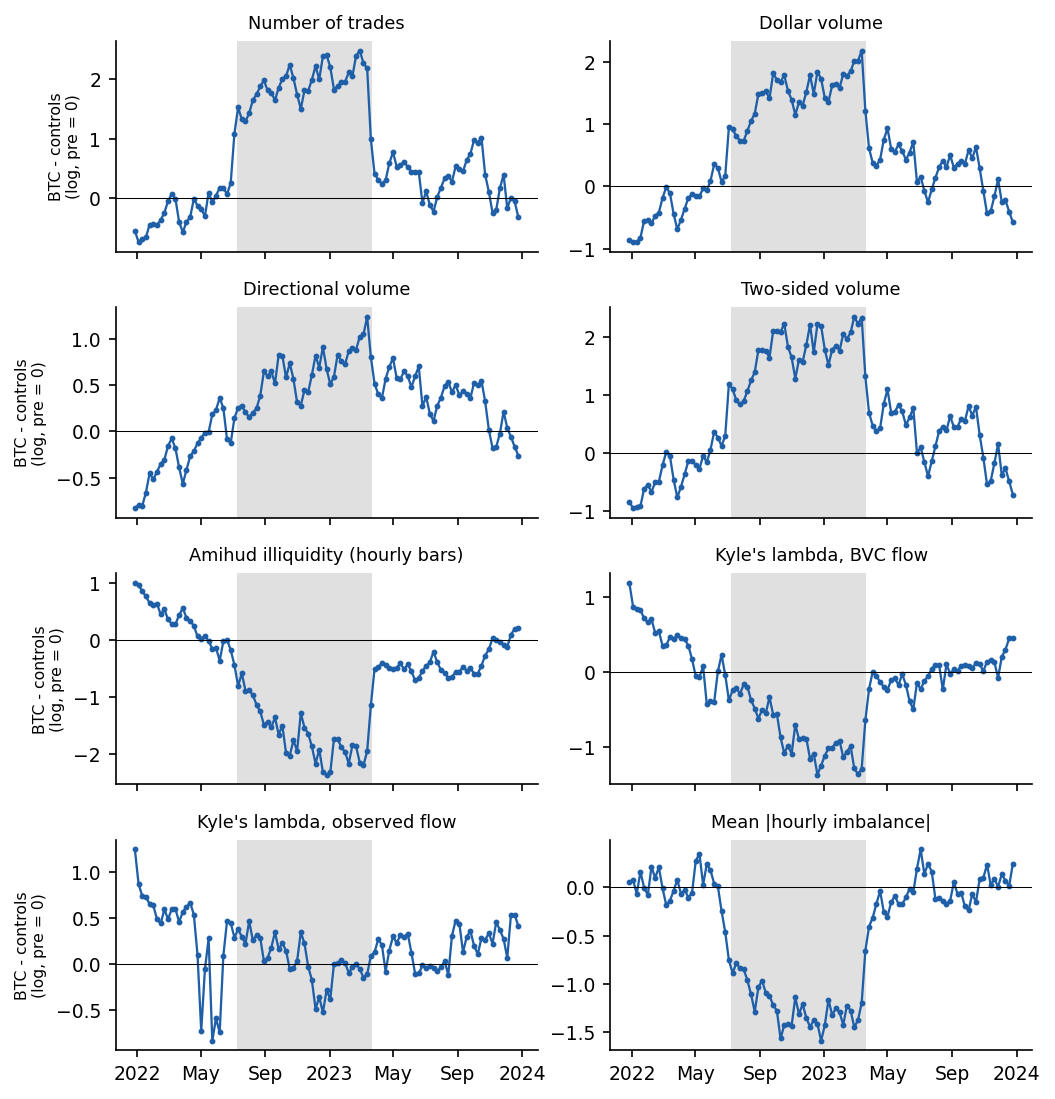
\includegraphics[width=0.95\textwidth]{fig_fee_event_study.png}
\caption{Weekly means of the BTC-minus-control difference for selected daily measures, January 2022 to
December 2023, relative to the 90 days before the promotion (log points). Shaded: zero fees on
BTC/USDT.}
\label{fig:feeevent}
\end{figure}

\section{Additional tables}

\begin{table}[H]
\centering\caption{Alternative flow classifiers vs.\ observed taker imbalance, BTC/USDT}\label{tab:variants}
\begin{tabular}{lrrrr}
\toprule
 & \multicolumn{2}{c}{Pearson} & \multicolumn{2}{c}{Same sign}\\
\cmidrule(lr){2-3}\cmidrule(lr){4-5} Classifier & 1h & 24h & 1h & 24h\\
\midrule
BVC Normal, sigma 24h (1h bars) & 0.503 & 0.516 & 0.716 & 0.695\\
BVC Normal, sigma 168h (1h bars) & 0.489 & 0.507 & 0.716 & 0.693\\
BVC Normal, sigma 720h (1h bars) & 0.484 & 0.505 & 0.716 & 0.691\\
BVC Student-t(3), sigma 168h (1h bars) & 0.494 & 0.507 & 0.716 & 0.687\\
Tick rule (1h bars) & 0.430 & 0.456 & 0.716 & 0.666\\
BVC Normal, sigma 1440m (1m bars) & 0.603 & 0.602 & 0.748 & 0.725\\
Tick rule (1m bars) & 0.597 & 0.617 & 0.728 & 0.731\\
\bottomrule
\end{tabular}

\tabnote{Correlation and sign agreement between proxy imbalance and observed taker imbalance, per hour
(1h) and over rolling 24-hour sums (24h). Student-$t$(3) is rescaled to unit variance.}
\end{table}

\begin{table}[H]
\centering\caption{Information ceiling by period}\label{tab:ceiling}
\begin{tabular}{lrrrrrr}
\toprule
Period & Hours & Ceiling & corr$^2$(BVC) & Slope & SD imb. & Ceiling (1m)\\
\midrule
\multicolumn{7}{l}{\emph{BTC/USDT}}\\
full sample & 42,315 & 0.247 & 0.239 & 0.128 & 0.130 & 0.338\\
zero-fee window & 6,154 & 0.374 & 0.360 & 0.038 & 0.030 & 0.345\\
standard fees & 36,161 & 0.267 & 0.257 & 0.142 & 0.140 & 0.362\\
2022 & 8,718 & 0.242 & 0.234 & 0.065 & 0.066 & 0.248\\
2023 & 8,757 & 0.278 & 0.253 & 0.106 & 0.099 & 0.370\\
2024 & 8,784 & 0.332 & 0.315 & 0.135 & 0.121 & 0.411\\
2025 & 8,760 & 0.281 & 0.265 & 0.167 & 0.165 & 0.362\\
2026 & 7,296 & 0.254 & 0.246 & 0.169 & 0.172 & 0.347\\
\multicolumn{7}{l}{\emph{ETH/USDT}}\\
full sample & 42,315 & 0.244 & 0.237 & 0.123 & 0.126 & 0.285\\
zero-fee window & 6,154 & 0.265 & 0.254 & 0.098 & 0.095 & 0.253\\
standard fees & 36,161 & 0.244 & 0.237 & 0.127 & 0.131 & 0.291\\
2022 & 8,718 & 0.283 & 0.275 & 0.094 & 0.091 & 0.211\\
2023 & 8,757 & 0.246 & 0.228 & 0.118 & 0.119 & 0.331\\
2024 & 8,784 & 0.319 & 0.307 & 0.129 & 0.118 & 0.336\\
2025 & 8,760 & 0.250 & 0.241 & 0.132 & 0.136 & 0.296\\
2026 & 7,296 & 0.212 & 0.199 & 0.147 & 0.163 & 0.270\\
\bottomrule
\end{tabular}

\tabnote{Ceiling: in-sample $R^2$ of observed hourly taker imbalance on 50 quantile-bin means of the
standardised bar return, the upper bound for any return-based classifier calibrated to that period.
corr$^2$(BVC): squared correlation of hourly BVC with observed imbalance. Slope: OLS slope of observed
imbalance on BVC (its calibration). SD imb.: standard deviation of observed hourly imbalance. Ceiling
(1m): the same bound for one-minute imbalance on one-minute returns.}
\end{table}

\begin{table}[H]
\centering\caption{BVC accuracy by regime, BTC/USDT}\label{tab:regimes}
\begin{tabular}{llrrrrr}
\toprule
 & & \multicolumn{2}{c}{Pearson} & \multicolumn{2}{c}{Same sign} & \\
\cmidrule(lr){3-4}\cmidrule(lr){5-6} Split & Group & 1h & 24h & 1h & 24h & Hours\\
\midrule
volatility & high vol & 0.499 & 0.619 & 0.715 & 0.744 & 13,119\\
volatility & low vol & 0.493 & 0.432 & 0.717 & 0.649 & 15,252\\
volatility & mid vol & 0.503 & 0.507 & 0.715 & 0.690 & 13,368\\
year & 2022 & 0.484 & 0.580 & 0.721 & 0.720 & 8,718\\
year & 2023 & 0.503 & 0.497 & 0.728 & 0.661 & 8,758\\
year & 2024 & 0.561 & 0.595 & 0.728 & 0.701 & 8,784\\
year & 2025 & 0.515 & 0.544 & 0.707 & 0.676 & 8,760\\
year & 2026 & 0.496 & 0.533 & 0.690 & 0.709 & 7,296\\
fee regime & standard fees & 0.507 & 0.524 & 0.710 & 0.693 & 36,148\\
fee regime & zero-fee promo & 0.600 & 0.595 & 0.749 & 0.690 & 6,168\\
\bottomrule
\end{tabular}

\tabnote{Volatility terciles use the 24h Garman-Klass volatility ranked against the trailing 30 days.}
\end{table}

\begin{table}[H]
\centering\caption{Rolling six-month estimation window, BTC/USDT}\label{tab:rolling}
\begin{tabular}{lrrrr}
\toprule
Model & Expanding $R^2_{OOS}$ & Rolling $R^2_{OOS}$ & Rolling CW $p$ & Rolling IC\\
\midrule
EN: TI & \ensuremath{-}0.055 & \ensuremath{-}0.411 & 0.52 & 0.001\\
EN: MS$_{\text{proxy}}$ & \ensuremath{-}0.139 & \ensuremath{-}0.379 & 0.73 & \ensuremath{-}0.007\\
EN: MS & \ensuremath{-}0.006 & \ensuremath{-}0.400 & 0.55 & \ensuremath{-}0.002\\
EN: ALL & \ensuremath{-}0.025 & \ensuremath{-}0.433 & 0.33 & \ensuremath{-}0.006\\
\bottomrule
\end{tabular}

\tabnote{Out-of-sample $R^2$ (\%) against the zero forecast with the expanding window of the main
analysis and with a six-month rolling window; Clark-West $p$-value and IC for the rolling window.}
\end{table}

\begin{table}[H]
\centering\caption{Drop-one-group ablation, full elastic net, BTC/USDT}\label{tab:dropgroup}
\begin{tabular}{lrrr}
\toprule
Group dropped & Features & $R^2_{OOS}$ (\%) & IC\\
\midrule
none (EN: ALL) & 45 & \ensuremath{-}0.025 & 0.019\\
spread impact & 41 & \ensuremath{-}0.115 & \ensuremath{-}0.004\\
order flow & 40 & \ensuremath{-}0.072 & 0.014\\
volatility & 39 & 0.021 & 0.018\\
efficiency structure & 39 & \ensuremath{-}0.169 & 0.006\\
activity & 43 & \ensuremath{-}0.045 & 0.011\\
trade level & 37 & \ensuremath{-}0.125 & 0.005\\
intrahour 1m & 41 & \ensuremath{-}0.118 & 0.017\\
\bottomrule
\end{tabular}

\end{table}

\begin{table}[H]
\centering\caption{Conditional out-of-sample accuracy, BTC/USDT}\label{tab:conditional}
\resizebox{\textwidth}{!}{\begin{tabular}{llrrrrr}
\toprule
Split & Group & Hours & EN: TI & EN: MS & EN: ALL & EN: Flow$_{\text{taker}}$\\
\midrule
vol regime & high & 11,647 & \ensuremath{-}0.150 (0.38) & \ensuremath{-}0.029 (0.47) & \ensuremath{-}0.080 (0.36) & \ensuremath{-}0.033 (0.72)\\
vol regime & low & 13,914 & 0.042 (0.05) & \ensuremath{-}0.056 (0.46) & 0.054 (0.06) & \ensuremath{-}0.087 (0.73)\\
vol regime & mid & 12,032 & 0.035 (0.05) & 0.085 (0.03) & 0.006 (0.12) & 0.005 (0.25)\\
illiq regime & high & 12,524 & \ensuremath{-}0.049 (0.17) & \ensuremath{-}0.026 (0.39) & 0.056 (0.12) & 0.002 (0.32)\\
illiq regime & low & 13,471 & 0.103 (0.03) & 0.070 (0.02) & 0.024 (0.08) & \ensuremath{-}0.043 (0.67)\\
illiq regime & mid & 11,598 & \ensuremath{-}0.254 (0.64) & \ensuremath{-}0.074 (0.65) & \ensuremath{-}0.181 (0.55) & \ensuremath{-}0.072 (0.85)\\
session & Asia 00-08 & 12,528 & \ensuremath{-}0.166 (0.33) & \ensuremath{-}0.086 (0.58) & \ensuremath{-}0.355 (0.73) & 0.002 (0.19)\\
session & Europe 08-16 & 12,533 & 0.014 (0.14) & 0.083 (0.03) & 0.134 (0.02) & \ensuremath{-}0.053 (0.83)\\
session & US 16-24 & 12,532 & \ensuremath{-}0.077 (0.23) & \ensuremath{-}0.076 (0.66) & \ensuremath{-}0.026 (0.23) & \ensuremath{-}0.038 (0.61)\\
weekend & weekday & 26,867 & \ensuremath{-}0.050 (0.13) & \ensuremath{-}0.005 (0.24) & 0.020 (0.05) & \ensuremath{-}0.043 (0.80)\\
weekend & weekend & 10,726 & \ensuremath{-}0.085 (0.16) & \ensuremath{-}0.010 (0.27) & \ensuremath{-}0.287 (0.52) & 0.007 (0.21)\\
fee regime & standard fees & 31,483 & \ensuremath{-}0.032 (0.05) & \ensuremath{-}0.001 (0.17) & \ensuremath{-}0.026 (0.08) & \ensuremath{-}0.026 (0.52)\\
fee regime & zero-fee (BTC/USDT promo) & 6,110 & \ensuremath{-}0.137 (0.64) & \ensuremath{-}0.023 (0.92) & \ensuremath{-}0.023 (0.92) & \ensuremath{-}0.072 (0.84)\\
\bottomrule
\end{tabular}
}
\tabnote{Out-of-sample $R^2$ against zero (\%) within each group, Clark-West $p$-value in parentheses.
Volatility and illiquidity terciles rank the 24h Garman-Klass volatility and the Amihud ratio against
the trailing 30 days, so group membership is known at forecast time.}
\end{table}

\begin{table}[H]
\centering\caption{Sub-period accuracy, BTC/USDT}\label{tab:subperiods}
\resizebox{\textwidth}{!}{\begin{tabular}{lrrrrrrr}
\toprule
Sub-period & BTC ret.\ (\%) & EN: TI & EN: MS$_{\text{proxy}}$ & EN: MS & EN: ALL & EN: Flow$_{\text{BVC}}$ & EN: Flow$_{\text{taker}}$\\
\midrule
2022-07-10--2023-08-14 & 36 & \ensuremath{-}0.162 & \ensuremath{-}0.354 & \ensuremath{-}0.018 & \ensuremath{-}0.019 & \ensuremath{-}0.228 & \ensuremath{-}0.057\\
2023-08-14--2024-09-08 & 84 & \ensuremath{-}0.086 & \ensuremath{-}0.035 & 0.045 & 0.034 & \ensuremath{-}0.058 & \ensuremath{-}0.068\\
2024-09-08--2025-10-05 & 132 & 0.319 & \ensuremath{-}0.011 & \ensuremath{-}0.050 & \ensuremath{-}0.079 & \ensuremath{-}0.008 & \ensuremath{-}0.016\\
2025-10-05--2026-10-31 & \ensuremath{-}38 & \ensuremath{-}0.272 & \ensuremath{-}0.137 & \ensuremath{-}0.009 & \ensuremath{-}0.052 & 0.000 & 0.012\\
\bottomrule
\end{tabular}
}
\tabnote{Out-of-sample $R^2$ against zero (\%) in four equal sub-periods of the test sample, with the
BTC return over each sub-period.}
\end{table}

\begin{table}[H]
\centering\caption{Out-of-sample forecast accuracy, ETH/USDT}\label{tab:forecast_eth}
\resizebox{\textwidth}{!}{\begin{tabular}{lrrrrcrr}
\toprule
Model & $R^2_{OOS}$ vs.\ 0 (\%) & $R^2_{OOS}$ vs.\ mean (\%) & CW $t$ vs.\ 0 & IC & 95\% CI & Hit rate & Hit $t$\\
\midrule
Historical mean & \ensuremath{-}0.083 & 0.000 & -- & \ensuremath{-}0.009 & [\ensuremath{-}0.028, 0.008] & -- & --\\
EN: TI & 0.102 & 0.186 & 2.97$^{***}$ & 0.012 & [\ensuremath{-}0.003, 0.029] & 0.499 & \ensuremath{-}0.20\\
EN: MS$_{\text{proxy}}$ & \ensuremath{-}0.266 & \ensuremath{-}0.182 & \ensuremath{-}1.60$$ & \ensuremath{-}0.005 & [\ensuremath{-}0.022, 0.011] & 0.495 & \ensuremath{-}0.83\\
EN: MS & \ensuremath{-}0.335 & \ensuremath{-}0.252 & \ensuremath{-}1.72$$ & 0.003 & [\ensuremath{-}0.015, 0.020] & 0.497 & \ensuremath{-}0.46\\
EN: ALL & \ensuremath{-}0.356 & \ensuremath{-}0.273 & \ensuremath{-}1.63$$ & \ensuremath{-}0.007 & [\ensuremath{-}0.025, 0.010] & 0.491 & \ensuremath{-}1.41\\
EN: Flow$_{\text{BVC}}$ & \ensuremath{-}0.083 & 0.001 & \ensuremath{-}0.34$$ & \ensuremath{-}0.014 & [\ensuremath{-}0.031, 0.003] & 0.491 & \ensuremath{-}1.91\\
EN: Flow$_{\text{taker}}$ & \ensuremath{-}0.010 & 0.073 & 1.06$$ & 0.009 & [\ensuremath{-}0.008, 0.026] & 0.505 & 1.08\\
GBM: MS & \ensuremath{-}0.441 & \ensuremath{-}0.357 & \ensuremath{-}0.32$$ & 0.002 & [\ensuremath{-}0.016, 0.017] & 0.501 & 0.25\\
GBM: ALL & \ensuremath{-}0.478 & \ensuremath{-}0.394 & \ensuremath{-}0.62$$ & \ensuremath{-}0.016 & [\ensuremath{-}0.034, 0.001] & 0.489 & \ensuremath{-}2.93\\
\bottomrule
\end{tabular}
}
\end{table}

\begin{table}[H]
\centering\caption{Incremental predictive information, ETH/USDT}\label{tab:incremental_eth}
\resizebox{\textwidth}{!}{\begin{tabular}{llcrrrrr}
\toprule
Model & Benchmark & Nested & $R^2_{OOS}$ rel.\ (\%) & CW $t$ & CW $p$ & DM $t$ & DM $p$\\
\midrule
EN: ALL & EN: TI & yes & \ensuremath{-}0.459 & \ensuremath{-}1.09$$ & 0.861 & \ensuremath{-}2.90$^{***}$ & 0.004\\
EN: MS & EN: TI & yes & \ensuremath{-}0.438 & \ensuremath{-}0.87$$ & 0.808 & \ensuremath{-}2.64$^{***}$ & 0.008\\
EN: MS & EN: MS$_{\text{proxy}}$ & yes & \ensuremath{-}0.069 & 0.37$$ & 0.354 & \ensuremath{-}0.71$$ & 0.478\\
EN: MS$_{\text{proxy}}$ & EN: TI & yes & \ensuremath{-}0.369 & \ensuremath{-}0.47$$ & 0.682 & \ensuremath{-}2.87$^{***}$ & 0.004\\
GBM: ALL & EN: TI & yes & \ensuremath{-}0.580 & \ensuremath{-}0.36$$ & 0.639 & \ensuremath{-}2.70$^{***}$ & 0.007\\
EN: Flow$_{\text{taker}}$ & EN: Flow$_{\text{BVC}}$ & no & 0.072 & -- & -- & 1.30$$ & 0.194\\
\bottomrule
\end{tabular}
}
\end{table}

\begin{table}[H]
\centering\caption{Return response to order-flow shocks, ETH/USDT}\label{tab:response_eth}
\begin{tabular}{lrrrrrr}
\toprule
Regressor (1 SD) & $k=1$h & $k=2$h & $k=4$h & $k=8$h & $k=12$h & $k=24$h\\
\midrule
Observed taker imbalance & 0.10 & \ensuremath{-}0.53 & 0.55 & 0.61 & 0.90 & 2.68\\
 & (0.33) & (\ensuremath{-}1.14) & (0.76) & (0.53) & (0.58) & (1.21)\\
BVC imbalance & 0.56 & 0.81 & 1.85 & 3.62 & 4.58 & 3.67\\
 & (1.10) & (1.10) & (1.74) & (2.29) & (2.36) & (1.31)\\
Observed imbalance, given $z_t$ & \ensuremath{-}0.15 & \ensuremath{-}0.79 & 0.21 & \ensuremath{-}0.41 & \ensuremath{-}0.46 & 2.10\\
 & (\ensuremath{-}0.45) & (\ensuremath{-}1.55) & (0.26) & (\ensuremath{-}0.31) & (\ensuremath{-}0.26) & (0.81)\\
Bar return $z_t$, given imbalance & 0.58 & 0.62 & 0.80 & 2.39 & 3.21 & 1.36\\
 & (1.10) & (0.85) & (0.76) & (1.61) & (1.69) & (0.51)\\
\bottomrule
\end{tabular}

\end{table}

\begin{table}[H]
\centering\caption{Proxy validation, ETH/USDT}\label{tab:validation_eth}
\resizebox{\textwidth}{!}{\begin{tabular}{lrrrr}
\toprule
 & Pearson & Spearman & Same sign & $N$\\
\midrule
\multicolumn{5}{l}{\emph{Panel A. Signed order flow: proxy vs.\ observed taker imbalance}}\\
BVC, 1h bars, per hour & 0.487 & 0.532 & 0.708 & 42,316\\
BVC, 1h bars, 4h sums & 0.470 & 0.530 & 0.708 & 42,310\\
BVC, 1h bars, 24h sums & 0.513 & 0.561 & 0.720 & 42,270\\
BVC, 1m bars summed to 1h & 0.556 & 0.605 & 0.735 & 42,359\\
Tick rule, 1h bars, per hour & 0.432 & 0.418 & 0.708 & 42,357\\
\midrule
\multicolumn{5}{l}{\emph{Panel B. Price impact and volatility}}\\
Kyle $\lambda$ (48h): BVC vs.\ observed flow & 0.440 & 0.503 & -- & 41,978\\
log GK vol (1h bars) vs.\ log RV (1m), 24h & 0.987 & 0.984 & -- & 41,978\\
\midrule
\multicolumn{5}{l}{\emph{Panel C. Information ceiling of return-based classifiers (out-of-sample $R^2$)}}\\
 & BVC raw & BVC rescaled & Any $f(z)$ & $N$\\
1h bars & \ensuremath{-}8.868 & 0.218 & 0.222 & 21,158\\
1m bars & \ensuremath{-}0.153 & 0.276 & 0.286 & 1,270,544\\
\midrule
\multicolumn{5}{l}{\emph{Panel D. Spread estimators (one tick $=$ 0.043 bps)}}\\
 & Median (bps) & Mean (bps) & Share $=0$ & Corr.\ log RV\\
Corwin-Schultz (24h mean) & 20.7 & 23.2 & 0.0\% & 0.85\\
Abdi-Ranaldo (24h) & 0.0 & 11.1 & 54.7\% & 0.61\\
Roll (48h) & 17.6 & 24.0 & 40.6\% & 0.52\\
\bottomrule
\end{tabular}
}
\end{table}

\begin{table}[H]
\centering\caption{BVC accuracy by regime, ETH/USDT}\label{tab:regimes_eth}
\begin{tabular}{llrrrrr}
\toprule
 & & \multicolumn{2}{c}{Pearson} & \multicolumn{2}{c}{Same sign} & \\
\cmidrule(lr){3-4}\cmidrule(lr){5-6} Split & Group & 1h & 24h & 1h & 24h & Hours\\
\midrule
volatility & high vol & 0.500 & 0.585 & 0.714 & 0.745 & 13,547\\
volatility & low vol & 0.478 & 0.468 & 0.697 & 0.699 & 15,050\\
volatility & mid vol & 0.510 & 0.541 & 0.715 & 0.717 & 13,142\\
year & 2022 & 0.525 & 0.666 & 0.713 & 0.758 & 8,718\\
year & 2023 & 0.478 & 0.462 & 0.700 & 0.678 & 8,758\\
year & 2024 & 0.554 & 0.575 & 0.727 & 0.733 & 8,784\\
year & 2025 & 0.491 & 0.541 & 0.703 & 0.725 & 8,760\\
year & 2026 & 0.446 & 0.477 & 0.693 & 0.701 & 7,296\\
fee regime & standard fees & 0.487 & 0.515 & 0.708 & 0.723 & 36,162\\
fee regime & zero-fee promo & 0.504 & 0.571 & 0.710 & 0.700 & 6,154\\
\bottomrule
\end{tabular}

\end{table}


\end{document}
